%  __________________________________________________________________
% |                                                                  |
% |                                                                  |
% |                      ChemFig Documentation                       |
% |                                                                  |
% |                       September 18, 2011                         |
% |                                                                  |
% |__________________________________________________________________|
%
% This is chemfig_doc_en.tex, the LaTeX code of the chemfig English
% documentation. Translation by Theo Hopman & Nikola Castillo
%
% Maintainer: Christian Tellechea
% E-mail    : unbonpetit@gmail.com
%             Comments, bug reports and suggestions are welcome.
% Licence   : Released under the LaTeX Project Public License v1.3c or
%             later, see http://www.latex-project.org/lppl.txt
% Copyright : Christian Tellechea 2010-2011
%
% The "chemfig" package consists of the 8 following files:
%   chemfig.tex (the code of the package)
%   chemfig.sty (the file for LaTeX)
%   t-chemfig.tex (the file for ConTeXt)
%   README
%   chemfig_doc_fr.tex, chemfig_doc_fr.pdf (french manual)
%   chemfig_doc_en.tex, chemfig_doc_en.pdf (english manual)
%
% -------------------------------------------------------------------
% This work may be distributed and/or modified under the
% conditions of the LaTeX Project Public License, either version 1.3
% of this license or (at your option) any later version.
% The latest version of this license is in
%
%     http://www.latex-project.org/lppl.txt
%
% and version 1.3 or later is part of all distributions of LaTeX
% version 2005/12/01 or later.
% -------------------------------------------------------------------
% This work has the LPPL maintenance status `maintained'.
%
% The Current Maintainer of this work is Christian Tellechea
% -------------------------------------------------------------------
\documentclass[10pt]{article}
\usepackage[utf8]{inputenc}
\usepackage[T1]{fontenc}
\usepackage[a4paper,margin=2.5cm,head=17pt,headsep=3mm,footskip=10mm]{geometry}
\usepackage[bottom]{footmisc}
\usepackage{libertine}
\renewcommand*\oldstylenums[1]{{\fontfamily{fxlj}\selectfont #1}}
\usepackage[scaled=0.8]{luximono}
\usepackage{amsmath}
\usepackage{array}
\usepackage{longtable}
\usepackage{xspace}
\usepackage{fancybox}
\usepackage{boites}
\usepackage{textcomp}
\usepackage{enumitem}
\usepackage{chemfig}
\usetikzlibrary{decorations.pathmorphing}
\usetikzlibrary{matrix}
\usepackage{siunitx}
\usepackage{emerald}
\usepackage{xstring}
\usepackage[protrusion=true,expansion,final,babel=true]{microtype}
\usepackage{fancyhdr}
\fancypagestyle{plain}{%
	\fancyhead[L]{\colorbox{gray!40}{\rlap{\small\bfseries\CF}\kern\dimexpr\linewidth-2\fboxsep}}
	\fancyhead[C]{}
	\fancyhead[R]{\scriptsize\slshape\leftmark\kern0.5em}
	\fancyfoot[l]{\tiny\LaTeX ed by Christian \textsc{Tellechea}, the \today.}
	\fancyfoot[c]{}
	\fancyfoot[r]{\thepage}}
\renewcommand\headrulewidth{0pt}

\makeatletter
\let\gobble\@gobble
\newcommand\idx{\@ifstar{\let\print@or@not\@gobble\idx@}{\let\print@or@not\@firstofone\idx@}}
\newcommand\idx@[1]{%
	\ifcat\expandafter\noexpand\@car#1\@nil\relax% si sc
		\expandafter\ifx\@car#1\@nil\protect
			\index{#1}%
			\print@or@not{#1}%
		\else
			\saveexpandmode\expandarg
			\StrSubstitute{\string#1}{\string @}{\@empty\protect\symbol{'100}}[\temp@]%
			\StrGobbleLeft\temp@1[\temp@]%
			\restoreexpandmode
			\expandafter\index\expandafter{\temp@ @\protect\texttt{\protect\textbackslash\temp@}}%
			\print@or@not{\texttt{\string#1}}%
		\fi
	\else
		\index{#1}%
		\print@or@not{#1}%
	\fi
}

\newcommand\make@car@active[2]{%
	\catcode`#1\active
	\begingroup
		\lccode`\~`#1\relax
		\lowercase{\endgroup\def~{#2}}%
}

\newif\if@exstar

\newcommand\exemple{%
	\begingroup
	\parskip\z@
	\@makeother\;\@makeother\!\@makeother\?\@makeother\:% neutralise frenchb
	\@ifstar{\@exstartrue\exemple@}{\@exstarfalse\exemple@}}

\newcommand\exemple@[2][65]{%
	\medbreak\noindent
	\begingroup
		\let\do\@makeother\dospecials
		\make@car@active\ { {}}%
		\make@car@active\^^M{\par\leavevmode}%
		\make@car@active\,{\leavevmode\kern\z@\string,}%
		\make@car@active\-{\leavevmode\kern\z@\string-}%
		\make@car@active\>{\leavevmode\kern\z@\string>}%
		\make@car@active\<{\leavevmode\kern\z@\string<}%
		\exemple@@{#1}{#2}%
}

\newcommand\exemple@@[3]{%
	\def\@tempa##1#3{\exemple@@@{#1}{#2}{##1}}%
	\@tempa
}

\newcommand\exemple@@@[3]{%
	\xdef\the@code{#3}%
	\endgroup
	\if@exstar
		\begingroup
			\fboxrule0.4pt
			\let\breakboxparindent\z@
			\def\bkvz@bottom{\hrule\@height\fboxrule}%
			\let\bkvz@before@breakbox\relax
			\def\bkvz@set@linewidth{\advance\linewidth\dimexpr-2\fboxrule-2\fboxsep}%
			\def\bkvz@left{\vrule\@width\fboxrule\hskip\fboxsep}%
			\def\bkvz@right{\hskip\fboxsep\vrule\@width\fboxrule}%
			\def\bkvz@top{\hbox to \hsize{%
				\vrule\@width\fboxrule\@height\fboxrule
				\leaders\bkvz@bottom\hfill
				\ECFAugie
				\fboxsep\z@
				\colorbox{black}{\kern0.25em\color{white}\footnotesize\lower0.5ex\hbox{\strut#2}\kern0.25em}%
				\leaders\bkvz@bottom\hfill
				\vrule\@width\fboxrule\@height\fboxrule}}%
			\breakbox
				\kern.5ex\relax
				\ttfamily\footnotesize\the@code\par
				\normalfont
				\kern3pt
				\hrule height0.1pt width\linewidth depth0.1pt
				\vskip5pt
				\rightskip0pt plus 1fill
				\everypar{{\color{lightgray}\rlap{\vrule height0.1pt width\linewidth depth0.1pt}}\hskip0pt plus 1fill}%
				\newlinechar`\^^M\everyeof{\noexpand}\scantokens{#3}\par
			\endbreakbox
		\endgroup
	\else
		\vskip0.5ex
		\boxput*(0,1)
			{\fboxsep\z@
			\hbox{\ECFAugie\colorbox{black}{\leavevmode\kern0.25em{\color{white}\footnotesize\strut#2}\kern0.25em}}%
			}%
			{\fboxsep5pt
			\fbox{%
				$\vcenter{\hsize\dimexpr0.#1\linewidth-\fboxsep-\fboxrule\relax
					\kern5pt\parskip0pt \ttfamily\footnotesize\the@code}%
				\vcenter{\kern5pt\hsize\dimexpr\linewidth-0.#1\linewidth-\fboxsep-\fboxrule\relax
					\everypar{{\color{lightgray}\rlap{\vrule height0.1pt width\dimexpr\linewidth-0.#1\linewidth-\fboxsep-\fboxrule depth0.1pt}}}%
					\footnotesize\newlinechar`\^^M\everyeof{\noexpand}\scantokens{#3}}$%
				}%
			}%
	\fi
	\medbreak
	\endgroup
}

\newcommand\falseverb[1]{{\ttfamily\detokenize{#1}}}

\long\def\centerverb#1{%
	\def\centerverb@i##1#1{##1\hfill\null\par\egroup}
	\bgroup
		\ttfamily\@noligs
		\parskip3.5pt\par\hfill
		\let\do\@makeother\dospecials
		\@vobeyspaces
		\centerverb@i}

\makeatother

\usepackage[english]{babel}
\def\degres{\ensuremath{{}^\circ}}

\newcommand\CF{{\ECFAugie ChemFig}\xspace}
\newcommand\TIKZ{ti\textit kz\xspace}
\newcommand\molht[1]{\begingroup\parskip3.5pt\par\hfill\chemfig{#1}\hfill\null\par\endgroup}
\newcommand\boxednode[2]{\fbox{$\mathrm{#1}\vphantom{M_1}$}_{#2}}
\newcommand\boxedfalseverb[1]{{\fboxsep0pt\fbox{\vphantom|\falseverb{#1}}}}

\usepackage[plainpages=false,pdfpagelabels,bookmarks=true,bookmarksopen=true,colorlinks=true,hyperfootnotes=false,filecolor=black,linkcolor=blue,urlcolor=magenta,pdfauthor={Christian TELLECHEA},pdftitle={ChemFig},pdfsubject={Draw 2D molecule with LaTeX},pdfkeywords={ChemFig},pdfcreator={LaTeX}]{hyperref}

\csname @addtoreset\endcsname{section}{part}
\usepackage{titlesec}
\titleformat{\part}[display]
	{\normalfont\Large\filcenter\sffamily\bfseries}%
	{\LARGE\MakeUppercase{\partname~\thepart}}%
	{1pc}%
	{\titlerule\vspace{1pc}\Huge}

\begin{filecontents*}{chemfig_doc_en.ist}
% Fichier de style makeindex
heading_prefix "{\\bfseries\\hfill "
heading_suffix "\\hfill\\null}\\nopagebreak\n"
headings_flag 1
symhead_positive "Symbols"
symhead_negative "Symbols"
delim_0 "\\dotfill"
delim_1 "\\dotfill"
delim_2 "\\dotfill"
\end{filecontents*}

\usepackage{makeidx}
\makeindex
\begin{document}
\begin{titlepage}
	\catcode`!12
	
\begin{tikzpicture}[remember picture,overlay]
		\shade [left color=blue,right color=white]([yshift=2cm]current page.west) rectangle ([xshift=-1cm]current page.south);
		\shade [left color=white,right color=blue] ([xshift=1cm]current page.south) rectangle ([yshift=2cm]current page.east);
		\filldraw[black](current page.north west) rectangle ([yshift=7cm]current page.east);
		\shade[top color=black,bottom color=blue]([yshift=7cm]current page.east)rectangle([yshift=2.5cm]current page.west);
		\filldraw[black!55!blue!100]([yshift=2.5cm]current page.east)rectangle([yshift=2cm]current page.west);
	\end{tikzpicture}
	\begin{center}
		\color{white}\ECFAugie\fontsize{50pt}{50pt}\selectfont\CF\par
		\Large v\csname CF@ver\endcsname\par\bigskip
		\footnotesize\csname CF@en@date\endcsname\par
		\normalsize Christian Tellechea\par\vskip1.5cm
		\huge A \TeX{} package for drawing molecules%
	\end{center}
	\vskip4cm
	\begin{center}
		\scriptsize
		\setatomsep{3em}%
		\chemfig{-[::-30](-[5])(-[7])-[::+60]-[::-60]O-[::+60](=[::-45]O)-[::+90]HN>:[::-60](-[::+60]**6(------))-[::-30](<:[2]OH)-[::-60](=[6]O)-[::+60]O>:[::-60]*7(---?(<[::-120]OH)-(<|[1]CH_3)(<:[::-90]CH_3)-(-[1](<[::+80]HO)-[0](=[::+60]O)-[7](<|[::+130]CH_3)(-[::+75](<|[2]OH)-[::-60]-[::-60](<[::+30]O-[::-90])-[::-60](<[::+90])(<:[::+30]O-[7](-[6]CH_3)=[0]O)-[::-60])-[6]-[5,1.3]?(<:[7]O-[5](=[::-60]O)-[6]**6(------)))=(-[2]CH_3)-)}%
		\par
		{\ECFAugie\small Taxotere}%
	\end{center}
	\vskip1.5cm
	\hfill
	\hbox to 0pt{\hss\scriptsize
		\setbondoffset{1pt}
		\setatomsep{2.5em}
		\setcompoundsep{5em}
		\setarrowoffset{6pt}
		\schemestart
		  \chemfig{(-[:-150]R')(-[:-30]R)=[2]N-[:30]OH}
		  \arrow{<=>[\chemfig{H^\oplus}]}
		  \chemfig{(-[@{a0}:-150]R')(-[:-30]R)=[2]@{a1}N-[@{b0}:30]@{b1}\chemabove{O}{\scriptstyle\oplus}H_2}
		  \chemmove[red,-stealth,red,shorten <=2pt]{
		      \draw(a0)..controls +(135:2mm) and +(215:4mm).. (a1);
		      \draw(b0)..controls +(120:2mm) and +(180:3mm).. ([yshift=7pt]b1.180);}
		  \arrow{<=>[\chemfig{{-}H_2O}]}[,1.1]
		  \chemleft[{\subscheme[90]{%
		    \chemfig{R'-\chemabove{N}{\scriptstyle\oplus}~C-R}
		    \arrow{<->}[,0.75]
		    \chemfig{R'-\lewis{2:,N}=@{a1}\chemabove{C}{\scriptstyle\oplus}-R}}}\chemright]
		  \arrow{<=>[\chemfig{H_2@{a0}\lewis{0:2:,O}}]}[,1.1]
		  \chemmove[red,-stealth,red,shorten <=3pt]{
		      \draw(a0)..controls+(90:10mm)and+(45:10mm)..([yshift=6pt]a1.45);}
		  \chemfig{*6(R\rlap{$'$}-N=(-R)-\chemabove{O}{\scriptstyle\oplus} H_2)}
		  \arrow{<=>[\chemfig{{-}H^\oplus}]}
		  \chemfig{*6(R\rlap{$'$}-N=(-R)-OH)}
		  \arrow
		  \chemfig{*6(R\rlap{$'$}-\chembelow{N}{H}-(-R)(=[2]O))}
		\schemestop\hss}\hfill\null
	\begin{center}
		\ECFAugie\small The Beckmann rearrangement%
	\end{center}
\end{titlepage}
\parindent0pt\pagestyle{plain}
\tableofcontents
\parskip\medskipamount
\vspace{2cm}

\setitemize{leftmargin=3em,topsep=0pt,parsep=0pt,itemsep=0pt}
\part{Introduction}
\section{New in version 1.0a}
Here is what is new in version 1.0a:
\begin{itemize}
	\item the \verb-\lewis- and \verb-\Lewis- macros have an optional argument which controls the offset of the Lewis drawings in the odd directions, see page~\pageref{opt.lewis};
	\item the \verb-\setlewisdist- macro sets the distance between the circles representing a pair of electrons, see page~\pageref{setlewisdist}.
\end{itemize}

\section{Foreword}
This package has seen the light of day thanks to the assistance of Christophe \textsc{Casseau}, who had the idea after being confronted with the complexity of the syntax of the \href{http://www.ctan.org/tex-archive/help/Catalogue/entries/ppchtex.html}{\texttt{\textbf{ppchtex}}} package.

Throughout the writing of the code, he helped me find interesting features. He always encouraged me to write more advanced features even though I was sometimes (nearly always?) reluctant; if \CF has the features it does, it is in large part thanks to him. I thank him as well for his testing of beta versions of this package, and for his contributions to the writing of this manual.\medskip

\begingroup
\leftskip0.1\linewidth
\rightskip0.1\linewidth
\itshape\small
Experience shows that is it has been difficult to combine drawing of molecules with the typographic quality of a program like \LaTeX, leaving little choice for the user who wishes to have a vector format for these drawings. After having abandoned the \emph{ppchtex} package (developed for con\TeX t and available under \LaTeX) because of the complexity of its syntax, I turned to the world of programs outside \LaTeX. The difficulty in this case is finding a compromise between quality and price. After many unsuccessful attempts I found the only option was a new package, and I would like to thank Christian \textsc{Tellechea} for bringing it to life. To meet my requirements, \CF needed to be easy to use but still have advanced features, something well nigh impossible. Yet he was able to put together a very flexible \TeX{} code which makes it a pleasure for me to write my molecules. I hope it will be the same for you readers looking for a package useful in the field of chemistry.\smallskip

\hfill Christophe \textsc{Casseau}\kern0.1\linewidth
\endgroup\medskip

Finally, I wish to warmly thank Theo \textsc{Hopman} and more recently Nikola \textsc{Castillo} for offering to translate this manual into English.

\section{Presenting \protect\CF}
To use this package, start by adding the following code to the preamble:
\begin{itemize}
	\item {\color{blue}\verb-\input chemfig.tex-} with $\varepsilon$\TeX\idx*\input;
	\item {\color{blue}\verb-\usepackage{chemfig}-} with \LaTeX\idx*{Latex@\protect\LaTeX}\idx*\usepackage;
	\item {\color{blue}\verb-\usemodule[chemfig]-} with Con\TeX t\idx*{ConTeXt@Con\protect\TeX{}t}\idx*\usemodule.
\end{itemize}

In all cases, the \TIKZ\idx*{tikz} package, if not loaded before, is loaded by \CF.

The most important command for drawing molecules is \verb|\chemfig{<code>}|\idx*\chemfig. The argument \verb|code| is a set of characters describing the structure of the molecule according to the rules which are described in this manual.

Care has been taken to make it possible to draw the greatest possible number of molecular configurations, while maintaining a simple, flexible, and intuitive syntax. Despite this, the \verb-<code>- which describes the 2D structure of the molecule increases in complexity in proportion to that of the molecule being drawn.

The command \verb|\chemfig| draws a molecule using the commands provided by the \TIKZ\idx*{tikz} package, placed inside a \verb|tikzpicture|\idx*{tikzpicture} environment. The choice of \TIKZ implies that:
\begin{itemize}
\item the user has a choice of compilation method\idx*{compilation method}: pdf\LaTeX{} can be used equally well in \idx{dvi mode} (tex $\longrightarrow$ dvi $\longrightarrow$ ps $\longrightarrow$ pdf) or in \idx{pdf mode} (tex $\longrightarrow$ pdf). In effect \TIKZ, via the underlying \idx{pgf}, gives identical graphical results in the two modes;
\item the \idx{bounding box} is automatically calculated by \TIKZ and the user need not worry about any overlap with the text. However, care must be taken with alignment when the molecule is drawn in a paragraph. In the following example, we have drawn the \idx{bounding box} for the molecule: {\fboxsep0pt \fbox{\chemfig{H_3C-C(-[:-30]OH)=[:30]O}}}. \CF always places the first atom of the molecule on the \idx{baseline} of the preceding code.
\end{itemize}
\newpage

\part{\protect\CF for the impatient}
This part is a non-exhaustive overview of the features of \CF. The goal is to introduce the basic ideas, allowing the user to get started drawing molecules as quickly as possible. This part does not go into detail; advanced use and a more formal approach to \CF commands will be discussed in the following parts.

\section{Syntax}
The command \verb|\chemfig|\idx*{\chemfig} is used in the following way:
\centerverb/\chemfig{<atom1><bond type>[<angle>,<coeff>,<n1>,<n2>,<tikz code>]<atom2>}/

\begin{itemize}
\item \verb-<angle>- is the bond angle\idx*{bond!angle} between the two atoms;
\item \verb-<coeff>- is a coefficient multiplying the default bond length\idx*{bond!length};
\item \verb-<n1>- and \verb-<n2>- are the numbers of the departure and arrival atoms of the bond\idx*{bond!departure and arrival atoms};
\item \verb-<tikz code>- is additional options concerning the colour or style of a bond\idx*{bond!customization}.
\end{itemize}
\medskip
Each bond takes optional arguments\idx*{bond!optional argument} which are placed in square brackets. These arguments can adjust everything one needs for the bond. Each argument has a default value, so one can simply write:
\exemple{The water molecule}|\chemfig{H-O-H}|

In all the examples, the grey line represents the \idx{baseline}.

\section{The different types of bonds}
\idx*{bond!types}For \CF, bonds between two atoms are one of nine types, represented by the characters \boxedfalseverb-, \boxedfalseverb=, \boxedfalseverb~, \boxedfalseverb>, \boxedfalseverb<, \boxedfalseverb{>:}, \boxedfalseverb{<:}, \boxedfalseverb{>|} and \boxedfalseverb{<|} :\label{types.liaisons}
\begin{center}
\begin{tabular}{>{\centering\arraybackslash}m{1.7cm}>{\centering\arraybackslash}m{3cm}>{\centering\arraybackslash}m{2cm}m{4cm}}
\hline
Bond \#&Code                 &Result      &Bond type\\\hline
1            &\verb+\chemfig{A-B}+ &\chemfig{A-B} &Single\\
2            &\verb+\chemfig{A=B}+ &\chemfig{A=B} &Double\\
3            &\verb+\chemfig{A~B}+ &\chemfig{A~B} &Triple\\
4            &\verb+\chemfig{A>B}+ &\chemfig{A>B} &right Cram, plain\\
5            &\verb+\chemfig{A<B}+ &\chemfig{A<B} &left Cram, plain\\
6            &\verb+\chemfig{A>:B}+&\chemfig{A>:B}&right Cram, dashed\\
7            &\verb+\chemfig{A<:B}+&\chemfig{A<:B}&left Cram, dashed\\
8            &\verb+\chemfig{A>|B}+&\chemfig{A>|B}&right Cram, hollow\\
9            &\verb+\chemfig{A<|B}+&\chemfig{A<|B}&left Cram, hollow\\\hline
\end{tabular}
\end{center}
\label{setdoublesep}The command \verb-\setdoublesep{<dim>}-\idx*{\setdoublesep} adjusts the spacing between the lines in double or triple bonds. This spacing is 2pt by default.

\section{Different types of diagrams}
\subsection{Complete structural diagram}
\exemple{Ethane}|\chemfig{C(-[2]H)(-[4]H)(-[6]H)-C(-[2]H)(-[6]H)-H}|

Each bond takes several optional arguments\idx*{bond!optional argument}. The first optional argument defines the \verb-<angle>- of the bond\idx*{bond!angle}. Angles increase counterclockwise. If no angle is give then its default value is 0\degres.

Note: the parentheses allow multiple bonds from the same atom; see ``Branched molecules''\idx*{branched molecule}, page~\pageref{molecules.ramifiees}.

There are many ways of specifying the angle of a bond.
\begin{description}
\item[Predefined angles] \idx*{bond!angle!predefined}When the optional argument contains a whole number, this represents the angle that the bond makes with the horizontal, in multiples of 45\degres.

\exemple{Predefined angles}|\chemfig{(-[1]1)(-[2]2)(-[3]3)(-[4]4)(-[5]5)(-[6]6)(-[7]7)-0}|

\item[Absolute angle] \idx*{bond!angle!absolute}To give an angle in degrees relative to the horizontal, the optional argument must take this form: \verb-[:<absolute angle>]-. The \verb-<absolute angle>- may be positive or negative, and may have decimal places. It is reduced to the interval $[0,360)$.
\item[Relative angle] \idx*{bond!angle!relative}It is often useful to give the bond angle relative to the preceding bond. In this case, the following syntax must be used:\verb-[::<relative angle>]-. The \verb-<relative angle>- may be positive or negative, and may have decimal places.
\end{description}

\subsection{Condensed structural diagram}
\exemple{Hex-1-ene}|\chemfig{H_3C-{{(CH_2)}_3}-CH=CH_2}|

It is sometimes useful to change the length of a bond\idx*{bond!length}. In the preceding example, the first two bonds need to be lengthened; they are too short compared to the double bond. To do this, the \verb|<coeff>| is needed in the optional arguments\idx*{bond!optional argument}.

\exemple{Hex-1-ene}|\chemfig{H_3C-[,1.5]{{(CH_2)}_3}-[,1.5]CH=CH_2}|

Notes:
\begin{itemize}
	\item in the notation \verb|[,1.5]|, the comma indicates that the value placed in brackets corresponds to the second argument (\verb|coeff|). To give a value for the fourth argument one would write \verb|[,,,2]|;
	\item characters between braces are not interpreted by \CF, which allows (for example) groupings of atoms to be written inside parentheses without having them treated as part of a branched molecule (see page~\pageref{molecules.ramifiees}).
\end{itemize}

\subsection{Cram representation}
\idx*{Cram representation}Another way of showing the bond angle between two atoms.
\exemple{Methane}|\chemfig{C(-[5]H)(-[2]H)(<[:-70]H)(<:[:-20]H)}|

\subsection{Skeleton diagram}
\idx*{skeleton diagram}The simplest input, only covalent bonds are listed with their possible settings.
\exemple{But-2-ene}|\chemfig{-[:30]=[:-30,,,,red]-[:30]}|

The double bond lines are drawn on either side of where the single bond line would be. To keep graphical consistency between skeleton diagrams of various compounds it is useful to shift the second double bond line above or below the single bond line\idx*{bond!shifted}. Just follow the \verb-=- symbol with \verb-^- or \verb-_-, as shown below:
\exemple{Comparison between double bonds and shifted double bonds}/\chemfig{-[:-30]=[:30]-[:-30]} \chemfig{-[:-30]=^[:30]-[:-30]}\par
\chemfig{=[:-30]-[:30]=[:-30]} \chemfig{=_[:-30]-[:30]=^[:-30]}/

\subsection{Lewis diagrams}
\idx*{Lewis diagram}The syntax is as follows:
\centerverb/\lewis{<position index><electron state>,<atom>}/
\smallskip

The electron states can be a lone pair, an empty electron slot, or a single electron. By default the electron state is a lone pair. A single electron is represented by the character \boxedfalseverb. and an empty slot by \boxedfalseverb|.

\exemple{Chloromethane and water}|\chemfig{C(-[2]H)(-[4]H)(-[6]H)-\lewis{260,Cl}}\hspace{1cm}
\chemfig{[:40]H-\lewis{13,O}-[::-80]H}|

Note: the positions take whole number values between 0 and 7.
\exemple{Positions}/\lewis{0.2.4.6.,C}\hspace{1cm}
\lewis{0|2.46.,C}\hspace{1cm}
\lewis{1357,Ar}/

\section{Branched molecules}\label{molecules.ramifiees}
\idx*{branched molecule}To indicate a branch, simply follow the atom holding the branch with a \verb-<code>- in parentheses. This \verb-<code>- is the code of the submolecule which will be attached to the atom. Multiple branches can be attached to the same atom, and these can be nested.

\exemple{Alkanes}|\chemfig{H_3C-CH(-[2]CH_3)-CH_3}
\hspace{.5cm}\chemfig{-(-[2])(-[6])-}|

In this type of representation it is sometimes necessary to connect to distant atoms\idx*{bond!distant atoms}. To do this, the character \verb|?| is used, which creates a hook between two atoms. The function
\centerverb/?[<name>,<bond>,<tikz>]/
takes three arguments: the name of the hook, the bond type, and tikz code. The following example shows how to make two different hooks.

\exemple*{Cocaine}|\chemfig{H_2C(-C?[a]H-[:-30]CH_2-[:30]C?[b]H-O-CO-C_6H_5)
-[2]CH_2-[,1.7]CH(-[3]N?[a]-[3]H_3C)(-[,1.35]C?[b]H-CO-OCH_3)}|

\section{Rings}
\idx*{ring}\CF can easily draw regular polygons. The syntax is the following:
\centerverb/\chemfig{*n(<code for the molecule>)}/
\smallskip

\exemple{Some rings}|
\chemfig{*3(---)}\hspace{.5cm}
\chemfig{*5(-=-=-)}\hspace{.5cm}
\chemfig{*6(-=-=-=)}|

\idx*{ring!branch}Branches are used in the same way as before.

\exemple{Rings and branches}|\chemfig{*4(-(--[1]*4(----))---)}|

Note: a ring does not start or finish with the atom or group of atoms with which one wants to close the ring. The chemical entity on which the ring is based must be outside the ring definition.

\exemple{Proper coding}|\chemfig{A*4(-B-C-D-)}|

\exemple{Bad coding}|\chemfig{*4(A-B-C-D-)}\hspace{1cm}
	\chemfig{*4(-B-C-D-A)}|

\section{Ions}
The \verb|chemfig| commands enters the \idx{math mode}\footnote{There is a problem with the placement of groups of atoms containing exponents or subscripts. See page~\pageref{alignement.vertical}.} of \TeX, so it is very simple to write an ion. A negative charge ($-$) must always be enclosed in braces to avoid \CF confusing it with the symbol for a single bond.

\exemple{Acetate ion}|\chemfig{-(-[1]O^{-})=[7]O}|

For purists it is possible to circle the charge of an ion by using the commands \verb|\ominus| and \verb|\oplus|\idx*{charge!\protect\texttt{\protect\string\protect\oplus}}\idx*{charge!\protect\texttt{\protect\string\protect\ominus}}.

To meet all requirements, there are two other commands \idx{\chemabove} and \idx{\chembelow} which allow placement of charges above or below the current atom\idx*\lewis.

\exemple{Some ions}|\chemfig{-(-[1]O^{\ominus})=[7]O}
\hspace{1cm}
\chemfig{\lewis{35,O}=\lewis{26,Cl}-\chemabove
{\lewis{026,O}}{\ominus}}
\vskip5pt
\chemfig{-\chemabove{N}{\scriptstyle\oplus}(=[1]O)-[7]O^{\ominus}}|

For those who are extremely picky, the commands \idx{\chemabove} and \idx{\chembelow} accept an optional argument which sets the distance between the charge and the atom\idx*\lewis.
\exemple{Charge position}|\chemfig{\lewis{35,O}=C-\chemabove
[3pt]{\lewis{246,O}}{\hspace{.5cm}\ominus}}|

\section{Chemical equations}
Here is an example of a \idx{chemical reaction}:
\exemple*{Chemical reaction}/\chemfig{**6(------)} \hspace{.5cm} + \hspace{.5cm} \chemfig{H_3C-Cl}
\hspace{.5cm} $\xrightarrow{catalyst}$ \hspace{.5cm} 
\chemfig{**6(---(-)---)} \hspace{.5cm} + \hspace{.5cm} \chemfig{H-Cl}/

\CF adds two new commands \idx{\chemsign} and \idx{\chemrel} which slightly simplify the preceding syntax.

\exemple*{Using the \CF commands}|\setchemrel{0pt}{1.2em}{6em}
\chemfig{**6(------)}\chemsign[0.5cm]+\chemfig{H_3C-Cl}
\chemrel[\itshape\tiny Catalyst]{->}
\chemfig{**6(---(-)---)}\chemsign[0.5cm]+\chemfig{H-Cl}|
\newpage

\part{Operation of \protect\CF}
This part is devoted to describing the most common features of \CF. The outline of this description far exceeds that of ``\CF for the impatient``, but the user will find here explanations sufficient to draw most molecules. The presentation of features is done from a theoretical angle, and the goal of this part is not to draw real molecules but to give the user a formal description of the functionality of \CF. The ``Advanced usage'', page~\pageref{utilisation.avancee}, will be more practical and will illustrate advanced features for the most demanding uses. It will also highlight methods of building real molecules, page~\pageref{exemples.commentes}. Finally, the last part will give examples of molecules and the code used to draw them.

\section{Groups of atoms}
Drawing a molecule consists inherently of connecting groups of atoms with lines. Thus, in the molecule \chemfig{O=O}, there are two groups of atoms, each consisting of a single atom ``O''.

{\fboxsep1pt
However, in this molecule
\molht{H_3C-C(-[:-30]OH)=[:30]O}
there are four groups of atoms: ``$\mathrm{H_3C}$'', ``C'', ``O'' and ``OH''. For reasons which we shall see later, \CF splits each group into single atoms. Each atom extends up to the next capital letter or one of these special characters: {\ttfamily \boxedfalseverb{-} \boxedfalseverb{=} \boxedfalseverb{~} \boxedfalseverb{(} \boxedfalseverb{!} \boxedfalseverb{*} \boxedfalseverb{<} \boxedfalseverb{>} \boxedfalseverb{@}}. \CF ignores all characters inside braces when splitting groups into atoms\idx*{separating atom mechanism}.

Therefore the first group of atoms ``$\mathrm{H_3C}$'' is split into two atoms: $\boxednode{H_3}{}$ and $\boxednode C{}$. In terms of chemistry, of course, these are not real atoms; $\mathrm{H_3}$, for example, consists of three hydrogen atoms. In what follows the word atom refers to \CF's definition. Thus \CF sees the preceding molecule as follows:
\renewcommand*\printatom[1]{\fbox{\ensuremath{\mathrm{#1}}}}
\molht{H_3C-[,1.75]C(=[:30,1.5]O)(-[:-30,1.5]OH)}}

\section{Different types of bonds}
\idx*{bond!types}As we have already seen (see page~\pageref{types.liaisons}), bonds can be one of nine types, each corresponding to the characters \boxedfalseverb-, \boxedfalseverb=, \boxedfalseverb~, \boxedfalseverb>, \boxedfalseverb<, \boxedfalseverb{>:}, \boxedfalseverb{<:}, \boxedfalseverb{>|} and \boxedfalseverb{<|}.

\label{longueur.liaison}\idx*{bond!length}We must understand that when a bond is made between two atoms, these atoms are contained within invisible rectangular boxes. The centres of these two rectangles are separated by an adjustable distance $\Delta$ called the ``interatomic distance''. Furthermore, bonds do not connect to the exact edges of the rectangles: a length $\delta$, also adjustable, separates the edges of the rectangles and the beginning and end of the bond line. The rectangular boxes are made visible in the diagram below to help understanding.
\begin{center}
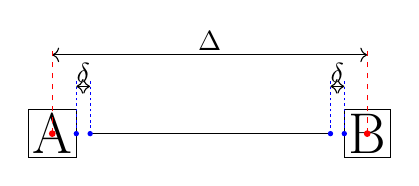
\begin{tikzpicture}[every node/.style={anchor=base,inner sep=1.5pt,outer sep=0pt,minimum size=0pt},baseline]
	\node[draw] at(0,0)(aa){\huge A};
	\node[draw]at(4,0)(bb){\huge B};
	\path[shorten <=5pt,shorten >=5pt,draw](aa)--(bb)coordinate[pos=0](al) coordinate[pos=1](bl);
	\node[draw,circle,fill,blue,minimum size=1.5pt,inner sep=0pt]at(al){};
	\node[draw,circle,fill,blue,minimum size=1.5pt,inner sep=0pt]at([xshift=5pt]al){};
	\node[draw,circle,fill,blue,minimum size=1.5pt,inner sep=0pt]at(bl){};
	\node[draw,circle,fill,blue,minimum size=1.5pt,inner sep=0pt]at([xshift=-5pt]bl){};
	\draw[blue,dash pattern=on 1pt off 1pt](bl)--([yshift=0.7cm]bl);
	\draw[blue,dash pattern=on 1pt off 1pt]([xshift=-5pt]bl)--([xshift=-5pt,yshift=0.7cm]bl);
	\draw[<->]([yshift=0.6cm]bl.center)--([xshift=-5pt,yshift=0.6cm]bl.center) node [midway,above,draw=none]{$\delta$};
	\draw[blue,dash pattern=on 1pt off 1pt](al)--([yshift=0.7cm]al);
	\draw[blue,dash pattern=on 1pt off 1pt]([xshift=5pt]al)--([xshift=5pt,yshift=0.7cm]al);
	\draw[<->]([yshift=0.6cm]al.center)--([xshift=5pt,yshift=0.6cm]al.center) node [midway,above,draw=none]{$\delta$};
	\node[draw,circle,fill,red,minimum size=2pt,inner sep=0pt]at(aa){};
	\node[draw,circle,fill,red,minimum size=2pt,inner sep=0pt]at(bb){};
	\draw[<->]([yshift=1cm]aa.center)--([yshift=1cm]bb.center) node [midway,above,draw=none] {$\Delta$} ;
	\draw[red,dash pattern=on 2pt off2pt](aa.center)--([yshift=1.1cm]aa.center);
	\draw[red,dash pattern=on 2pt off2pt](bb.center)--([yshift=1.1cm]bb.center);
\end{tikzpicture}
\end{center}

\label{setatomsep}The macro \verb-\setatomsep{<dimension>}-\idx*{\setatomsep} adjusts the interatomic distance $\Delta$. If the \verb-<dimension>- is empty, it takes the default value of 3em. This command, like all other settings commands, affects all the following molecules. 

\exemple{Interatomic distance}|\setatomsep{2em}\chemfig{A-B}\par
\setatomsep{50pt}\chemfig{A-B}|

\label{setbondoffset}\idx*{\setbondoffset}The command \verb-\setbondoffset{<dimension>}- sets the spacing $\delta$ between the bond line and the atom. If the \verb-<dimension>- is empty, $\delta$ takes the default value of 2pt.
\exemple{Trimming bonds}|\setbondoffset{0pt}\chemfig{A-B}\par
	\setbondoffset{5pt}\chemfig{A-B}|

If one bond is followed immediately by another, then \CF inserts an empty group \verb-{}-. Around this empty group the separation $\delta$ is zero:
\exemple{Empty groups}/\chemfig{A-B=-=C}/

\label{setbondstyle}\idx*{\setbondstyle}The \verb-\setbondstyle{<tikz code>}- command sets the style for all the bonds drawn thereafter. The \verb-<tikz code>- is empty by default. To custom a single bond, see page~\pageref{perso-liaisons}.
\exemple{Style of bonds}/\setbondstyle{line width=1pt,red}
\chemfig{A-B=C>|D<E>:F}/

\label{modif.retrait} The spacing $\delta$ for just one bond can be specified with the character \verb-#-\idx*{\protect\symbol{'043}@\protect\texttt{\protect\symbol{'043}}}. This character must be placed \emph{immediately} after the bond symbol and has one required argument between parentheses of the form ``\verb-#(<dim1>,<dim2>)-'', where \verb-<dim1>- is the spacing $\delta$ at the beginning of the bond and \verb-<dim2>- is the that at the end. If \verb-<dim2>- is omitted, the spacing at the end of the bond takes the value of $\delta$ in effect at that time. One can see in the example how the shortening, set to 4pt to be more visible, is nullified for the bond arriving at ``B'', then for the one leaving ``B'', and finally for both:
\begingroup
\catcode`\#12
\exemple{Fine adjustment of bond shortening}/\setbondoffset{4pt}
\chemfig{A-B-C}\par
\chemfig{A-#(,0pt)B-C}\par
\chemfig{A-B-#(0pt)C}\par
\chemfig{A-#(,0pt)B-#(0pt)C}/
\endgroup

By default, all atoms within groups of atoms are typeset in \idx{math mode} (spaces are ignored). They may therefore contain math mode specific commands such as subscripts or superscripts\footnote{There is a problem with the placement of groups of atoms containing exponents or subscripts. See page~\pageref{alignement.vertical}.}:
\exemple{Math mode}|\chemfig{A_1B^2-C _ 3 ^ 4}|

There are settings specifically for Cram bonds\idx*{Cram representation}\idx*\setcrambond. This syntax is used: \label{setcrambond}
\centerverb/\setcrambond{<dim1>}{<dim2>}{<dim3>}/
\smallskip

Any empty argument takes its default value. The three arguments are:
\begin{itemize}
	\item \verb-<dim1>- is the size of the base of the triangle, and is 1.5pt by default;
	\item \verb-<dim2>- is the thickness of the dots, and is 1pt by default;
	\item \verb-<dim3>- is the spacing between the dots, and is 2pt by default.
\end{itemize}

Here is an example where the three dimensions are changed:

\exemple{Modified Cram bonds}-\setcrambond{10pt}{0.4pt}{1pt}
	\chemfig{A>B>:C>|D}-

\section{Bond angle}
\idx*{bond!angle}\idx*{bond!optional argument|(}Each bond takes an optional argument in brackets. This optional argument can adjust every aspect of a bond, and consists of five optional fields separated by commas. The first of these fields defines the bond angle. Angles increase counterclockwise, and are relative to the horizontal. If the angle field is empty, the angle takes its default value of 0\degres. We will see later how to change this default.

There are several ways of specifying the bond angle.
\subsection{Predefined angles}
\idx*{bond!angle!predefined}When the angle field contains an integer, this represents the angle the bond makes relative to the horizontal, in multiples of 45\degres. For example, \verb-[0]- specifies an angle of 0\degres, \verb-[1]- is 45\degres, and so on up to \verb-[7]- which specifies an angle of 315\degres. The integer may lie outside the interval $[0,7]$, in which case the angle is reduced to the interval $[0,360)$.

\exemple{Predefined angles}|\chemfig{A-B-[1]C-[3]-D-[7]E-[6]F}|

These angles remain valid if the atoms are empty, and this is the case for all the features we will see below:
\exemple{Predefined angles with empty groups}|\chemfig{--[1]-[3]--[7]-[6]}|

\subsection{Absolute angles}
\idx*{bond!angle!absolute}If one wishes to specify an angle in degrees relative to the horizontal, then the optional angle field must take this form: \verb-[:<absolute angle>]-. If necessary, the \verb-<absolute angle>- is reduced to the interval $[0,360)$:
\exemple{Absolute angles}/\chemfig{A-[:30]B=[:-75]C-[:10]D-[:90]>|[:60]-[:-20]E-[:0]~[:-75]F}/

\subsection{Relative angles}\label{angle.relatif}
\idx*{bond!angle!relative}It is often useful to specify a bond angle relative to the preceding bond. This syntax must be then be used: \verb-[::<relative angle>]-. The sign of the \verb-<relative angle>- can be omitted if it is a \verb-+-.

Here is a molecule where the first bond has an absolute angle of $-5\degres$, and the rest of the bond angles are incremented by 20\degres:
\exemple{Result of relative angles}|\chemfig{A-[:-5]-[::+20]-[::20]B-[::+20]-[::20]C-[::20]}|

One can ``break'' a chain of relative angles by putting an absolute or predefined angle where desired. Here, atom ``B'' is followed by a bond at  an absolute angle of 315\degres.
\exemple{Result of relative angles followed by absolute}|\chemfig{A-[:-5]-[::20]-[::20]B-[7]-[::20]C-[::20]}|

\section{Length of a bond}
\idx*{bond!length}Rather than speaking of length of a bond, we should use the term interatomic spacing. If effect, only the interatomic spacing is adjustable with \idx{\setatomsep} as we have seen on page~\pageref{longueur.liaison}. Once this parameter is set, the length of a bond depends on the content of atoms and, to a lesser extent, the angle the bond makes with the horizontal. It should be obvious that two ``slimmer'' atoms will have larger edge separations than two which are larger. This can be seen easily in the following example where an ``I'' atom is narrower than an ``M'' atom, which means that the bond between the ``I'' atoms is longer than that between the ``M'' atoms:
\exemple{Influence of the size of atoms}|\chemfig{I-I}\par
\chemfig{M-M}|

This aspect of the size of atoms becomes particularly acute when the atom involves subscripts or superscripts. In this example, the bond is extremely short, to the point of confusion with a negative sign $-$:
\exemple{Too-short bond}|\chemfig{A^{++}_{2}-B^{-}_3}|

It is important to note that the exponent \verb+-+ is \emph{put inside braces}. If this were not done, \CF would stop the atom on this character, which is a bond character. The atom would then be ``\verb-B^-'', which would lead to unexpected results.

We see in the example above that is it sometimes necessary to increase (or perhaps reduce) the interatomic distance associated with a bond. For this, the optional argument to bonds is actually made up of several comma-separated fields. As we have seen, the first field specifies the angle.
The second field, if it is not empty, is a coefficient which multiplies the default interatomic distance $\Delta$. Thus, writing \verb+-[,2]+ asks that this bond have the default angle (first field is empty) and that the atoms it connects be separated by twice the default distance\idx*{bond!length}.
\exemple{Modified bond length}/\chemfig{A^{++}_{2}-[,2]B^{-}_3}\par
\chemfig{A-B-[,2]C=[,0.5]D}\par
\chemfig{-=[,1.5]-[,0.75]=[:-20,2]}/

We can change the \idx{size of molecules} by altering the font size or the argument of \idx{\setatomsep}, possibly on both \footnote{You can also use the second optional argument of \texttt{\string\chemfig}, see page~\pageref{arguments.optionnels}.}, being careful to confine these changes within a group if we want to limit the scope:
\exemple{How to modify the size of molecule}/\normalsize       \chemfig{H-[:30]O-[:-30]H}\par
\setatomsep{2.5em}\chemfig{H-[:30]O-[:-30]H}\par
\small            \chemfig{H-[:30]O-[:-30]H}\par
\footnotesize     \chemfig{H-[:30]O-[:-30]H}\par
\scriptsize       \chemfig{H-[:30]O-[:-30]H}\par
\tiny             \chemfig{H-[:30]O-[:-30]H}/

\section{Departure and arrival atoms}
\idx*{bond!departure and arrival atoms}A group of atoms can contain several atoms. Suppose we want to connect the group ``ABCD'' to the group ``EFG'' with a bond. \CF calculates which atom of the first group and which of the second group are to be connected by looking at the angle of bond relative to the horizontal. If the angle is between (but not including) $-90\degres$ and 90\degres{} (modulo 360\degres) then the bond is made between the last atom of the first group and the first atom of the second group. In all other cases, the bond is made between the first atom of the first group and the last atom of the second group.

Here are some examples where the bond is in the interval $(-90,90)$, and where the bond is made between D and E:
\exemple{Default atom connections}|\chemfig{ABCD-[:75]EFG}\quad
	\chemfig{ABCD-[:-85]EFG}\quad
	\chemfig{ABCD-[1]EFG}|

In the  following examples, the angles are in the interval $[90,270]$ and so the bond is made between A and G:
\exemple[60]{Default atom connections}|\chemfig{ABCD-[:100]EFG}\quad
	\chemfig{ABCD-[:-110]EFG}\quad
	\chemfig{ABCD-[5]EFG}|

One may sometimes want the bond partners to be atoms other than those determined by \CF. The departure and arrival atoms can be set with the optional bond argument by writing:
\centerverb/[,,<integer 1>,<integer 2>]/
\smallskip

where \verb-<integer 1>- and \verb-<integer 2>- are the numbers of the desired departure and arrival atoms. These atoms must exist, otherwise an error message will be given.
\exemple{Specified atom connections}|\chemfig{ABCD-[:75,,2,3]EFG}\qquad
	\chemfig{ABCD-[:75,,,2]EFG}\qquad
	\chemfig{ABCD-[:75,,3,2]EFG}|

\section{Customization of bonds}\label{perso-liaisons}
\idx*{bond!customization}There is a fifth and last optional argument for bonds which is found after the fourth comma:
\centerverb/[,,,,<tikz code>]/
\smallskip

\idx*{tikz}This \verb-<tikz code>- is passed directly to \TIKZ when the bond is drawn. There one can put characteristics such as colour (\verb-red-), dash type (\verb-dash pattern=on 2pt off 2pt-), thickness (\verb-line width=2pt-), or even decoration if the \TIKZ decoration library has been loaded. A bond can be made invisible by writing ``\verb-draw=none-''\idx*{bond!invisible}. To set several attributes, the syntax of \TIKZ is used, separating them by a comma:
\exemple{Passing tikz code}|\chemfig{A-[,,,,red]B}\par
	\chemfig{A-[,,,,dash pattern=on 2pt off 2pt]B}\par
	\chemfig{A-[,,,,line width=2pt]B}\par
	\chemfig{A-[,,,,red,line width=2pt]B}|

Numerous \TIKZ decoration libraries are available. For example, one can use the ``\verb-pathmorphing-'' library by putting \verb-\usetikzlibrary{decorations.pathmorphing}- in the preamble in order to draw wavy bonds:
\exemple{Wavy bonds}|\chemfig{A-[,3,,,decorate,decoration=snake]B}|

Cram bonds ignore thickness and dash settings.

\section{Default values}
\idx*{chemfig@\protect\texttt{\protect\string\protect\chemfig}}At the beginning of each molecule, the default values for the optional arguments are initialized. They are:
\begin{itemize}
	\item 0\degres{} for the bond angle;
	\item 1 for the length multiplication coefficient;
	\item \verb-<empty>- for the numbers of the departure and arrival atoms, which lets \CF calculate these based on the bond angle;
	\item \verb-<empty>- for the parameters passed to \TIKZ.
\end{itemize}

These default values can be changed for the whole molecule by beginning the molecule code with
\centerverb/[<angle>,<coeff>,<n1>,<n2>,<tikz code]/
\smallskip

Thus, if the code of a molecule begins with \verb-[:20,1.5]-, then all the bonds will be at angle of 20\degres{} by default, and the interatomic distances will have a length 1.5 times the default length. These default values can be overridden at any time by giving an optional argument, such as for the bond which follows atom ``C'' in this example:
\exemple{Overriding default values}|\chemfig{[:20,1.5]A-B-C-[:-80,0.7]D-E-F}|

If something odd like \verb-[1,1.5,2,2,red,thick]- is written, then unless otherwise indicated all the bonds will have an angle of 45\degres{}, the interatomic distances will be 1.5 times the default distance, the bonds will begin and end on the second atom of each group, and the bonds will be red and thick:
\exemple{Default values}|\chemfig{[1,1.5,2,2,red,thick]ABC-DEF=GHI}|\idx*{bond!optional argument|)}

\section{Branches}\idx*{branched molecule}
\subsection{Principle}
Up to now, all the molecules have been linear, which is rare. A sub-molecule can be attached to an atom by following the atom with \verb-<code>- in parentheses. This \verb-<code>- is the code of the submolecule which will be attached to the atom.

In this example, the sub-molecule ``\verb/-[1]W-X/'' will be attached to atom ``B'': 
\exemple{A branch}|\chemfig{A-B(-[1]W-X)-C}|

There can be several sub-molecules which are to be attached to the same atom. Just have several parentheses containing the code for each sub-molecule:
\exemple{Multiple branches}|\chemfig{A-B(-[1]W-X)(-[6]Y-[7]Z)-C}|

The code of each sub-molecule can define its own default values, which will be valid throughout the whole sub-molecule. Here a sub-molecule ``\verb/[:60]-D-E/'' is attached to atom ``B'', with a default angle of 60\degres{} absolute. A second sub-molecule ``\verb/[::-60,1.5]-X-Y/'' is attached to ``B'' with a default bond angle 60\degres{} less than that of the preceding bond (which will be the one between ``A'' and ``B'') and with an interatomic distance 1.5 times the default value:
\exemple{Default values in branches}|\chemfig{A-B([:60]-D-E)([::-30,1.5]-X-Y)-C}|

Observe what happens if, at the beginning of the main molecule, one writes ``\verb/[:-45]/'':
\exemple{Effect of the default bond angle}|\chemfig{[:-45]A-B([:60]-D-E)([::-30,1.5]-X-Y)-C}|

We see that the angle between the bond \verb/B-C/ and the bond \verb/B-X/ stays at 30\degres{} because it is a relative angle for the sub-molecule ``\verb/-X-Y/''. By contrast, the branch ``\verb/-D-E/'' stays inclined at 60\degres{} to the horizontal, and does not follow the rotation given by the $-45\degres$ angle at the beginning; this is expected because ``\verb/-D-E/'' has an absolute angle. It is essential that all the angles be relative in order to rotate the whole molecule.

\subsection{Nesting}
Sub-molecules may be nested, and the rules seen in the preceding paragraphs stay in force:
\exemple{Nested branches}|\chemfig{A-B([1]-X([2]-Z)-Y)(-[7]D)-C}|

\subsection{Method}
Suppose now that we want to draw an acid anhydride molecule:
\chemfig{R-C(=[::+60]O)-[::-60]O-[::-60]C(=[::+60]O)-[::-60]R}

The best way to get this is to find the longest chain. Here, for example, we can draw the chain \verb/R-C-O-C-R/ taking into account angles and using only relative angles:
\exemple{Acid anhydride structure}|\chemfig{R-C-[::-60]O-[::-60]C-[::-60]R}|

To this structure we just have to add two ``\verb/=O/'' sub-molecules to each of the carbon atoms:
\exemple{Acid anhydride}|\chemfig{R-C(=[::+60]O)-[::-60]O-[::-60]C(=[::+60]O)-[::-60]R}|

Because we used only relative angles, we can rotate this molecule by giving a default angle of e.g. 75\degres:
\exemple[70]{Rotation of a molecule}|\chemfig{[:75]R-C(=[::+60]O)-[::-60]O-[::-60]C(=[::+60]O)-[::-60]R}|

\section{Connecting distant atoms}
\idx*{bond!distant atoms}We have seen how to connect atoms \emph{which are adjacent in the code}. It is often necessary to connect atoms which are not next to each other in the code. Let's call these particular bonds ``distant bonds''.

Let's take this molecule:
\exemple{Branched structure}|\chemfig{A-B(-[1]W-X)(-[7]Y-Z)-C}|

and suppose that we want to connect the atoms \verb/X/ and \verb/C/. In this case, \CF allows a ``hook'' to be placed \emph{immediately} after the atom of interest. The character used for a hook is ``\verb-?-'' because of its similarity to a hook. So, if one writes \verb/X?/ then the atom \verb/X/ will have a hook. Later in the code, all atoms followed by a \verb-?- will be connected to \verb/X/:
\exemple{Distant bond}|\chemfig{A-B(-[1]W-X?)(-[7]Y-Z)-C?}|

We could connect other atoms to X by following them with \verb-?-. Here it's the atoms \verb-C- and \verb-Z-:
\exemple{Several distant bonds}|\chemfig{A-B(-[1]W-X?)(-[7]Y-Z?)-C?}|

Now imagine if we were to leave the distant bonds \verb/X-C/ and \verb/X-Z/while adding another: \verb/A-W/. We must therefore ask for two \emph{different} hooks, one on \verb/A/ and the other on \verb/X/. Fortunately the character \verb/?/ has an optional argument:
\centerverb/?[<name>,<bond>,<tikz>]/
\smallskip

where each field takes its default value if it is empty:
\begin{itemize}
	\item The \verb-<name>- is the name of the hook: all alphanumeric characters (a\dots z, A\dots Z, 0\dots 9) are allowed\footnote{This is not exactly right. Actually all the characters that can be put between \texttt{\string\csname...\string\endcsname} are allowed.}. The name is \verb-a- by default. In the first occurrence of the hook with this name, only this field is used.
	\item \verb-<bond>- specifies how the atom with the current occurrence of the named hook is to be bonded to the atom with the first occurrence of the hook. There are two ways this can be done. First, this field can be an integer representing the desired bond type: 1=single bond, 2=double bond, etc. (See the table on page~\pageref{types.liaisons} for the bond codes.)

		Second, the field can be one of the bond character codes, provided that this character is \emph{between braces}.
	\item \verb-<tikz>- will be passed directly to \TIKZ as we have seen with regular bonds.
\end{itemize}

Here is our molecule with the required distant bonds, then with the bond \verb/A-W/ and \verb/X-C/ customized:
\exemple{Multiple distant bonds}|\chemfig{A?[a]-B(-[1]W?[a]-X?[b])(-[7]Y-Z?[b])-C?[b]}\par\medskip
	\chemfig{A?[a]-B(-[1]W?[a,2,red]-X?[b])(-[7]Y-
	Z?[b,1,{line width=2pt}])-C?[b,{>},blue]}|

Several different hooks can be written after an atom. Suppose that in this unfinished pentagon, we wish to connect \verb/A-E/, \verb/A-C/ and \verb/E-C/:
\exemple{An incomplete ring}|\chemfig{A-[:-72]B-C-[:72]D-[:144]E}|

Then we must do this:
\exemple{Multiple distant bonds}|\chemfig{A?[a]-[:-72]B-C?[a]?[b]-[:72]D-[:144]E?[a]?[b]}|

\section{Rings}\idx*{ring|(}
The preceding example shows how to draw a regular polygon, but the method used is tedious because the angles depend on the number of sides of the polygon.

\subsection{Syntax}
\CF can easily draw regular polygons. The idea is to attach a ring to an \verb/<atom>/ outside the ring with this syntax:
\centerverb/<atom>*<n>(<code>)/
\smallskip

\verb/<n>/ is the number of sides of the polygon and the \verb/<code>/ describes the bonds and groups of atoms which make up its edges and vertices. This code \emph{must} begin with a bond because the atom is outside the ring.

Here is a 5-ring, attached to the atom ``\verb/A/'':
\exemple{5-ring}|\chemfig{A*5(-B=C-D-E=)}|

A ring can also be drawn with one, several, or all the groups of atoms empty, as is the case for diagrams outside rings:
\exemple{5-ring with empty groups}|\chemfig{*5(-=--=)}|

A ring can be incomplete\idx*{ring!unfinished}:
\exemple{Incomplete 5-ring}|\chemfig{*5(-B=C-D)}|
If a ring has a code which contains too many bonds and atom groups for the given number of vertices, all the bonds and groups over the maximum allowed are ignored:
\exemple{Truncated 5-ring}|\chemfig{A*5(-B=C-D-E=F-G=H-I)}|

It is possible to draw a circle or an arc in the inside of a ring\idx*{ring!inside arc}. To do so, the following syntax is used:
\centerverb/<atom>**[<angle 1>,<angle 2>,<tikz>]<n>(<code>)/
\smallskip

where each field of the optional argument takes its default value if it is empty:
\begin{itemize}
	\item \verb/<angle 1>/ and \verb/<angle 2>/ are the absolute angles of the start and finish of the arc. These default to 0\degres{} and 360\degres{} respectively so that a circle is drawn by default;
	\item \verb/<tikz>/ is the code that will be passed to \TIKZ for drawing the arc.
\end{itemize}

\exemple{Rings and arcs}|\chemfig{**6(------)}\quad
	\chemfig{**[30,330]5(-----)}\quad
	\chemfig{**[0,270,dash pattern=on 2pt off 2pt]4(----)}|

\subsection{Angular position}
\subsubsection{At the start}
\idx*{ring!angular position}As can be seen in the examples above, the rule is that the attachment atom ``\verb/A/'' is always at the south-west of the ring. Furthermore, the ring is always constructed counterclockwise, and the last bond descends vertically onto the attachment atom:
\exemple{Angular position of rings}|\chemfig{A*4(-B-C-D-)}\qquad\chemfig{A*6(------)}|

If this angular position is not convenient, it is possible to specify another angle using the optional argument at the beginning of the molecule. Here is a 6-cycle which has been rotated by $+30\degres$, by $-30\degres$, and lastly by $+60\degres$:
\exemple[55]{Rotation of rings}|\chemfig{[:30]A*6(------)}\qquad
	\chemfig{[:-30]A*6(------)}\qquad
	\chemfig{[:60]A*6(------)}|

\subsubsection{After a bond}
When a ring does not begin a molecule and one or more bonds have already been drawn, the default angular position changes: the ring is drawn is such a way that the bond ending on the attachment atom bisects the angle formed by the first and last sides of the ring.

Here is a simple case:
\exemple{Bond ending on a ring}|\chemfig{A-B*5(-C-D-E-F-)}|

The rule remains valid, whatever the angle of the preceding bond:
\exemple{Bonds ending on a ring}|\chemfig{A-[:25]B*4(----)}\vskip5pt
	\chemfig{A=[:-30]*6(=-=-=-)}|

\subsection{Branches on a ring}
\idx*{ring!branch}To have branches attached to the vertices of a ring, we use the syntax we have already seen:
\centerverb/<atom>(<code>)/
\smallskip

where the \verb/<code>/ is that of the sub-molecule and the \verb-<atom>- is at the vertex. Unique to rings, the default angle of the sub-molecule is not 0\degres{} but is calculated so that it will bisect the sides leaving the vertex:
\exemple{Branch on a ring}|\chemfig{X*6(-=-(-A-B=C)=-=-)}|

A sub-molecule can be attached to the first vertex of a ring, just like the other vertices:
\exemple{Ring and branches}|\chemfig{*5((-A=B-C)-(-D-E)-(=)-(-F)-(-G=)-)}|

If one wants the bond leaving a vertex not to be the bisector of its sides, one can tinker with the optional global parameter or the optional bond parameter:
\exemple[50]{Branches at specified angles}|\chemfig{*5(---([:90]-A-B)--)}\qquad
	\chemfig{*5(---(-[:90]A-B)--)}\qquad
	\chemfig{*5(---([::+0]-A-B)--)}|

It is worth noting that in the third example, where a relative angle of 0\degres{} was given, the bonds of the branch are drawn in line with the preceding bond in the ring. This is the rule on page~\pageref{angle.relatif} which specified that the reference angle was that of the bond last drawn.

We can now connect together rings with bonds:
\exemple{Connected rings}|\chemfig{*6(--(-*5(----(-*4(----))-))----)}|

\subsection{Nested rings}
\idx*{ring!nested}To ``glue'' two rings together, the syntax is only slightly different: the vertex is specified where the other ring is going to start. Simply follow this vertex by the usual syntax for a ring. Here for example is a 5-ring which is attached to the second vertex of a 6-ring:
\exemple{Nested rings}|\chemfig{A*6(-B*5(----)=-=-=)}|

Note that the ring which is going to be attached to the main ring has an angular position such that two of the rings' sides coincide. In addition, the 5-ring has only four bonds ``\verb/----/''. In effect, the fifth will be useless because it is the second side of the 6-ring, which has already been drawn.

It is quite possible to glue multiple rings together:
\exemple{Multiple nested rings}|\chemfig{*5(--*6(-*4(-*5(----)--)----)---)}|

There is a case where a trick must be used. It can be seen in this example that the fourth side of the second 5-ring just passes through the centre of atom ``\verb-E-''.
\exemple{Flawed drawing}|\chemfig{A-B*5(-C-D*5(-X-Y-Z-)-E-F-)}|

This is normal because the second 5-ring (which is attached to atom ``\verb-D-'') is drawn \emph{before} \CF knows about atom ``\verb-E-''. In this case, it is necessary to use two hooks to draw the bond \verb/Z-E/:
\exemple{Distant bond and ring}|\chemfig{A-B*5(-C-D*5(-X-Y-Z?)-E?-F-)}|

We could also use a \verb-\phantom{E}- at the last vertex of the 5-ring:
\exemple{Using \string\phantom}/\chemfig{A-B*5(-C-D*5(-X-Y-Z-\phantom{E})-E-F-)}/

\subsection{Rings and groups of atoms}
Some care must be taken with rings when one or more vertices are made up of groups of atoms:
\exemple{Ring and groups of atoms}|\chemfig{AB*5(-CDE-F-GH-I-)}|

In order for the ring to have a regular shape, it is necessary to override the \CF mechanism which automatically calculates the departure and arrival atoms of bonds\idx*{bond!departure and arrival atoms}. Here, \verb/C-F/ and \verb/F-G/ must be connected by using the optional argument\idx*{bond!optional argument} of these bonds:
\exemple{Forced departure and arrival atoms}|\chemfig{AB*5(-CDE-[,,1]F-[,,,1]GH-I-)}|\idx*{ring|)}

\section{Representing electron movements}\label{mecanismes-reactionnels}\idx*{electron movements|(}
Starting with \CF version 0.3, we can represent the movement of electrons in mesomeric effects or reaction mechanisms. This is done by marking the departure and arrival points of the electron movement arrow using the syntax ``\verb-@{<argument>}-''\idx*{"@}. This syntax allows a \TIKZ node to be placed and makes this node accessible outside the argument of the \verb-\chemfig- command thanks to the ``\texttt{remember picture}'' option which is passed to all the ``\idx{tikzpicture}'' environments. It is assumed that the viewer supports ``\idx{picture remembering}'' and that the compilation is done twice.

Two types of diagrams can arise, so we can ask for:
\begin{itemize}
	\item a zero size node on a bond using the syntax ``\verb-@{<name>,<coeff>}-'' placed at the beginning of the optional argument of the relevant bond, without being followed by a comma if there is a first optional argument. In this case, the node takes the name ``\verb-<name>-'' and the \verb-<coeff>-, which must be between 0 and 1, determines where the node is located on the bond. If ``\verb-@{<name>}-'' is used, the \verb-<coeff>- is set to 0.5 by default, which means that the node is placed halfway along the bond;
	\item a node on an atom using the syntax ``\verb-@{<name>}-'' immediately before the relevant atom. In this case, the node has exactly the same footprint as the atom, but may be empty and therefore have zero dimensions.
\end{itemize}
Once the \idx{\chemfig} command has drawn the molecule(s) and has placed the nodes with the syntax described above, we can connect these nodes to each other with \TIKZ instructions. These instructions are placed in the argument of the command \verb-\chemmove-\idx*{chemmove@\protect\texttt{\protect\string\protect\chemmove}|(}\footnote{Actually, the \texttt{\string\chemmove} command puts its argument in a ``\idx{tikzpicture}'' environment with the options ``\texttt{remember picture, overlay}''.} and has the following syntax if (for example) we need to connect a node named ``\verb-<name1>-'' to the node named ``\verb-<name2>-'':
\centerverb|\chemmove[<opt>]{\draw[<tikz opt>](<name1>)<tikz link>(<name2>);}|
\smallskip

The optional argument \verb-<opt>- of the \verb-\chemmove- command will be added to the argument of the \idx{tikzpicture} environment in which the links between the nodes will be drawn. The \verb-<tikz opt>- and \verb-<tikz link>- instructions are describe in detail in the documentation of the \TIKZ package.

\subsection{Mesomeric effects}
To make these concepts concrete, let's take the example of a mesomeric effect involving a double bond and non-bonding lone pair conjugate. Let's begin with the possible delocalization of electrons from the double bond. We will place a node named ``db'' (double bond) in the middle of the double bond and a node named ``a1'' on the end of the double bond.

\exemple{Mesomeric effect 1}/\chemfig{@{a1}=_[@{db}::30]-[::-60]\lewis{2,X}}
\chemrel{<->}
\chemfig{\chemabove{\vphantom{X}}{\ominus}-[::30]=_[::-60]
\chemabove{X}{\scriptstyle\oplus}}
\chemmove{\draw[->](db).. controls +(80:8mm) and +(145:8mm).. (a1);}/

As noted above, there is no comma after the node placed in the optional arguments of a bond; we write ``\verb|=_[@{db}::30]|'' and not ``\verb|=_[@{db},::30]|'' as one might be tempted to do.

To link the nodes ``db'' and ``a1'' we have used the following syntax:
\centerverb|\chemmove{\draw[->](db)..controls +(80:8mm) and +(145:8mm)..(a1);}|
\medskip

In this example we ask for an arrow (\verb/[->]/) and we use two \idx{control points}\footnote{To find all the ways of connecting two nodes with \TIKZ, read the documentation for that package.}. These will be located using polar coordinates at 80\degres{} and 8~mm from ``db'' for the first and at 145\degres{} and 8~mm from ``a1'' for the second. Though this syntax may seem complicated at first reading, one need not be alarmed because its use will usually be a matter of copying and pasting. Only the names and coordinates of the control points need be changed, as can be verified from the example below, where an arrow has been added from the lone pair (node ``dnl'' to the single bond (node ``sb'').
\exemple{Mesomeric effect 2}/\chemfig{@{a1}=_[@{db}::30]-[@{sb}::-60]@{dnl}\lewis{2,X}}
\chemrel{<->}
\chemfig{\chemabove{\vphantom{X}}{\ominus}-[::30]=_[::-60]
\chemabove{X}{\scriptstyle\oplus}}
\chemmove{
    \draw[->](db)..controls +(100:5mm) and +(145:5mm)..(a1);
    \draw[->](dnl)..controls +(90:4mm) and +(45:4mm)..(sb);}/

For our new arrow we have set the \idx{control points} as follows: 4~mm at an angle of 90\degres{} from ``dnl'' and 4~mm at an angle of 45\degres{} from ``sb''. But we are not completely satisfied, since we would like the arrow not to touch the line segment representing the lone pair. To do this we will add some options to our arrow.
\exemple{Mesomeric effect 3}/\chemfig{@{a1}=_[@{db}::30]-[@{sb}::-60]@{dnl}\lewis{2,X}}
\chemrel{<->}
\chemfig{\chemabove{\vphantom{X}}{\ominus}-[::30]=_[::-60]
\chemabove{X}{\scriptstyle\oplus}}
\chemmove[->]{
    \draw(db).. controls +(100:5mm) and +(145:5mm).. (a1);
    \draw[shorten <=3pt,shorten >=1pt](dnl) .. controls +(90:4mm)
          and +(45:4mm) .. (sb);}/

The option ``\verb|shorten <=3pt|'' indicates that the tail of the arrow is to be shortened by 3~pt just as ``\verb|shorten >=2pt|'' means that the head of the arrow is shortened by 2~pt.

We can use all the power of \TIKZ instructions to modify the style of the arrow. Here we change the head of the arrow leaving the double bound, writing ``\verb|-stealth|'' instead of ``\verb|->|'', and we draw the arrow with a fine dashed red line. We also add the letter $\pi$ above the middle of the arrow:
\exemple{Mesomeric effect 4}/\chemfig{@{a1}=_[@{db}::30]-[@{sb}::-60]@{dnl}\lewis{2,X}}
\chemrel{<->}
\chemfig{\chemabove{\vphantom{X}}{\ominus}-[::30]=_[::-60]
\chemabove{X}{\scriptstyle\oplus}}
\chemmove{
    \draw[-stealth,thin,dash pattern= on 2pt off 2pt,red]
        (db).. controls +(100:5mm) and +(145:5mm)..
        node[sloped,above] {$\pi$} (a1);
    \draw[->, shorten <=3pt, shorten >= 1pt]
        (dnl).. controls +(90:4mm) and +(45:4mm).. (sb);}/

In the following example, we'll see how to indicate the position of the departure or arrival anchor points of the arrow. If we write
\exemple{Departure or arrival anchor point 1}/\chemfig{@{x1}\lewis{1:,X}}
\hspace{2cm}
\chemfig{@{x2}\lewis{2|,X}}
\chemmove{\draw[->,shorten >=4pt]
    (x1).. controls +(90:1cm) and +(90:1cm).. (x2);}/

Note that the tail of the arrow does not leave correctly from our electrons; it leaves from the middle of the upper edge of the node. Indeed, we chose a departure angle of 90~\degres{} and so \TIKZ makes the arrow leave from the anchor ``x1.90'' which corresponds to the intersection of the ray leaving from the centre of node ``x1'' at a 90\degres{} angle relative to the horizontal and of the edge of the rectangular node. To get the arrow departure angle that we want, we must specify its position. After some trial and error, it is ``x1.57'':
\exemple{Departure or arrival anchor point 2}/\chemfig{@{x1}\lewis{1:,X}}
\hspace{2cm}
\chemfig{@{x2}\lewis{2|,X}}
\chemmove{\draw[->,shorten <=4pt,shorten >=4pt]
    (x1.57).. controls +(60:1cm) and +(120:1cm).. (x2);}/

In some cases it will be easier to use Cartesian coordinated for the \idx{control points}. Here we use just one control point placed 1~cm to the right of and 1.5~cm above ``x1'':
\exemple{A single control point}/\chemfig{@{x1}\lewis{1:,X}}
\hspace{2cm}
\chemfig{@{x2}\lewis{2|,X}}
\chemmove{\draw[->,shorten <=4pt,shorten >=4pt]
    (x1.57).. controls +(1cm,1.5cm).. (x2);}/

All the graphics drawn by means of the command \verb|\chemmove| are superimposed and will not be included in the bounding boxes. We can see this in the preceding example.

\subsection{Reaction mechanisms}
Thanks to the option \verb|remenber picture| which is passed to all the ``tikzpicture'' environments we can easily draw arrows indicating reaction mechanisms. Let's take for example the first step of the esterification reaction\idx*{charge!\protect\texttt{\protect\string\protect\oplus}}.
\exemple{Esterification: step 1}/\setatomsep{7mm}
\setchemrel{}{}{5mm}
\chemfig{R-@{dnl}\lewis{26,O}-H}
\chemsign{+}
\chemfig{R-@{atoc}C([6]-OH)=[@{db}]O}
\chemrel[\chemfig{@{atoh}\chemabove{H}{\scriptstyle\oplus}}]{<>}
\chemmove[->,shorten <=2pt]{
    \draw[shorten >=2pt](dnl)..controls +(90:1cm)and+(north:1cm)..(atoc);
    \draw[shorten >=6pt](db)..controls +(north:5mm)and+(100:1cm)..(atoh);}/

The use of the \verb|\chemabove{<code>}{<materiel>}|\idx*{\chemabove} command does not change the dimensions of the \idx{bounding box} of \verb|<code>|. For this reason we can run into some difficulty in pointing to the symbol representing the charge carried ($\oplus$ or $\ominus$). In the example above the solution is to create a control point\idx*{control points} with an angle of 110\degres{} at 1~cm from ``atoh'' and to shorten the arrow by 6pt. In the following example, the second step of the esterification reaction, we can see that the arrow can take more complicated forms without complicating the code.
\exemple{Esterification: step 2}/\setatomsep{7mm}
\setchemrel{}{}{5mm}
\chemfig{R-O-C(-[2]R)(-[6]OH)-@{dnl}\lewis{26,O}H}\hspace{1cm}
\chemfig{@{atoh}\chemabove{H}{\scriptstyle\oplus}}
\chemmove{
    \draw[->,shorten <=2pt, shorten >=7pt]
        (dnl).. controls +(south:1cm) and +(north:1.5cm).. (atoh);}/

The rest is left as an exercise to the reader\idx*{chemmove@\protect\texttt{\protect\string\protect\chemmove}|)}\idx*{electron movements|)}\dots.

\section{Writing a name under a molecule}\label{chemname}
For convenience, \CF can write the name of a molecule underneath it with the command\idx*\chemname
\centerverb/\chemname[<dim>]{\chemfig{<code of the molecule>}}{<name>}/
\smallskip

The \verb-<dim>-, which is 1.5ex by default, will be inserted between the \idx{baseline} of the molecule and the top of the letters of the \verb-<name>-. The \verb-<name>- will be centred relative to the molecule, but the \verb-<name>- may not contain multiple paragraphs. As we see in this example: \chemname{\chemfig{H-O-H}}{\scriptsize\bfseries The water molecule: $\mathrm{\mathbf{H_2O}}$}, the \verb-<name>- which is displayed under the molecule is taken into account only for the vertical size of the bounding box. The horizontal size of \verb-<name>- is always zero.

Here is a reaction with the names under the molecules\idx*{chemical reaction}:
\exemple*{Displaying names of molecules}/
\chemname{\chemfig{R-C(-[:-30]OH)=[:30]O}}{Carboxylic acid}
\chemsign{+}
\chemname{\chemfig{R'OH}}{Alcohol}
\chemrel{->}
\chemname{\chemfig{R-C(-[:-30]OR')=[:30]O}}{Ester}
\chemsign{+}
\chemname{\chemfig{H_2O}}{Water}/

There are some limitations to this command. Suppose we switch the acid and the alcohol on the left side:
\exemple*{Name alignment 1}/
\chemname{\chemfig{R'OH}}{Alcohol}
\chemsign{+}
\chemname{\chemfig{R-C(-[:-30]OH)=[:30]O}}{Carboxylic acid}
\chemrel{->}
\chemname{\chemfig{R-C(-[:-30]OR')=[:30]O}}{Ester}
\chemsign{+}
\chemname{\chemfig{H_2O}}{Water}/

In fact, to draw the \verb-<name>- the command \idx{\chemname} inserts 1.5ex${}+{}$\emph{the largest of the depths\footnote{In \TeX{} terms, the depth is the dimension which extends vertically below the baseline.} of the molecules thus far} below the baseline of each molecule (light grey for the examples in this manual). The command \idx{\chenameinit}\verb-{<stuff>}- initializes this largest depth with the \verb-<stuff>-. Therefore one should:
\begin{itemize}
	\item write \verb-\chemnameinit{<deepest molecule>}- before using the \verb-\chemname- command in a reaction, unless the reaction begins with the deepest molecule;
	\item write \verb-\chemnameinit{}- after having written all the names in a chemical reaction lest the greatest depth in this reaction interfere with a future reaction.
\end{itemize}

Thus the correct code uses \idx{\chemnameinit} before and after the reaction:
\exemple*{Name alignment 2}/
\chemnameinit{\chemfig{R-C(-[:-30]OH)=[:30]O}}
\chemname{\chemfig{R'OH}}{Alcohol}
\chemsign{+}
\chemname{\chemfig{R-C(-[:-30]OH)=[:30]O}}{Carboxylic acid}
\chemrel{->}
\chemname{\chemfig{R-C(-[:-30]OR')=[:30]O}}{Ester}
\chemsign{+}
\chemname{\chemfig{H_2O}}{Water}
\chemnameinit{}/

Finally, to write a name on multiple lines, the command \verb-\\-\idx*{\protect\symbol{'134}\protect\symbol{'134}@\protect\texttt{\protect\symbol{'134}\protect\symbol{'134}}} encountered in a \verb-<name>- causes a line break\footnote{Conversely, the command \texttt{\textbackslash par} is forbidden and causes a compilation error.}:
\exemple*{Name on 2 lines}/
\chemname{\chemfig{R-C(-[:-30]OH)=[:30]O}}{Carboxylic\\acid}
\chemsign{+}
\chemname{\chemfig{R'OH}}{Alcohol}
\chemrel{->}
\chemname{\chemfig{R-C(-[:-30]OR')=[:30]O}}{Ester}
\chemsign{+}
\chemname{\chemfig{H_2O}}{Water}
\chemnameinit{}/
\newpage

\part{Advanced usage}\label{utilisation.avancee}
\section{Separating atoms}\label{decoupage.atomes}
The \idx{separating atom mechanism} described previously extends each atom until the next capital letter or one of the characters {\ttfamily \boxedfalseverb{-} \boxedfalseverb{=} \boxedfalseverb{~} \boxedfalseverb{(} \boxedfalseverb{!} \boxedfalseverb{*} \boxedfalseverb{<} \boxedfalseverb{>} \boxedfalseverb{@}}

In certain cases this automatic separation produces incorrect atoms which can translate into an imperfect diagram. Consider this example molecule, noting that the ``\texttt('' character is placed between braces so that \CF doesn't incorrectly create a branch:

\exemple*{Alkene}/\chemfig{CH_3CH_2-[:-60,,3]C(-[:-120]H_3C)=C(-[:-60]H)-[:60]C{(}CH_3{)}_3}/

We find that the bond which arrives at the carbon atom in the upper right is too short. This happens because, if we apply the \CF rules for separating atoms\idx*{separating atom mechanism} to the upper right group, the atoms are split in this way: ``\texttt{\detokenize{C{(}}}'', ``\texttt{\detokenize{C}}'', ``\texttt{\detokenize{H_3{)}_3}}''. We now realize that the first atom contains a parenthesis and thus has too great a depth in math mode; we can see this by making the bounding boxes visible:
\begin{center}
\fboxsep=0pt
\renewcommand*\printatom[1]{\fbox{\ensuremath{\mathrm{#1}}}}%
\chemfig{CH_3CH_2-[:-60,,3]C(-[:-120]H_3C)=C(-[:-60]H)-[:60]C{(}CH_3{)}_3}%
\end{center}
The character ``|'' forces splitting of the atom when it is encountered. Thus we can write \texttt{C\textcolor{red}{|}\detokenize{{(CH_3)_3}}} to ensure that \CF separates just two atoms here: ``\texttt{\detokenize{C}}'' and ``\texttt{\detokenize{{(CH_3)_3}}}''. The problem of the too-short bond is thus solved:

\exemple*{Alkene}/\chemfig{CH_3CH_2-[:-60,,3]C(-[:-120]H_3C)=C(-[:-60]H)-[:60]C|{(CH_3)_3}}/

\section{Displaying atoms}\label{perso.affichage}
Once a molecule has been split into atoms, the macro \idx{\printatom} is called internally by \CF in order to display each atom. Its sole argument is the code of the atom to be displayed (e.g. ``\verb-H_3-''). By default, this macro enters \idx{math mode} and displays its argument with the math font family ``rm''. It is defined by the following code:
\begin{itemize}
	\item \verb|\newcommand*\printatom[1]{\ensuremath{\mathrm{#1}}}|\qquad when compiling with \LaTeX{}\idx*{Latex@\protect\LaTeX}
	\item \verb|\def\printatom#1{\ifmmode\rm#1\else$\rm#1$\fi}|\qquad when compiling with $\varepsilon$\TeX{}\idx*{etex@$\protect\varepsilon$\protect\TeX} ou Con\TeX tX\idx*{ConTeXt@Con\protect\TeX{}t}.
\end{itemize}

One can modify the code of this macro to customize how atoms are displayed. In the following example, we redefine \idx{\printatom} so that each atom will be enclosed in a rectangular box:
\exemple{Redefinition of \string\printatom}/\fboxsep=1pt
\renewcommand*\printatom[1]{\fbox{\ensuremath{\mathrm{#1}}}}
\chemfig{H_3C-C(=[:30]O)(-[:-30]OH)}/

Here is how to redefine it to use the ``sf'' font family of math mode:
\exemple{Atoms displayed with ``sf'' font family}/\renewcommand*\printatom[1]{\ensuremath{\mathsf{#1}}}
\chemfig{H_3C-C(=[:30]O)(-[:-30]OH)}/

\section{Optional arguments}\label{arguments.optionnels}
The \idx{\chemfig} command takes two optional arguments\idx*{chemfig@\protect\texttt{\protect\string\protect\chemfig}!optional arguments}; their syntax is as follows:
\centerverb|\chemfig[<opt1>][<opt2>]{<molecule code>}|
\smallskip

The first optional argument \verb-<opt1>- contains \TIKZ instructions which will be passed to the \idx{tikzpicture} environment in which the molecule is drawn. The second optional argument \verb-<opt2>- contains \TIKZ instructions which will be executed when each node\footnote{These instructions are added to the end of the argument of \texttt{every node/.style\{<argument>\}}. This argument contains by default the following instructions: ``{\ttfamily anchor=base,inner sep=0pt,outer sep=0pt,minimum size=0pt}''.} is drawn.

With the use of the first optional argument one can, for example, choose the global colour or thickness of lines:
\exemple{Style choice}/\chemfig{A-B-[2]C}\par\medskip
\chemfig[line width=1.5pt]{A-B-[2]C}\par\medskip
\chemfig[red]{A-B-[2]C}/

With the second optional argument, one can choose the colour of nodes drawn by \TIKZ, change the angle of the drawing or its scale\idx*{size of molecules}:
\exemple{Style choices}/\chemfig{A-B-[2]C}\par\medskip
\chemfig[][red]{A-B-[2]C}\par\medskip
\chemfig[dash pattern=on 1pt off 2pt][red]{A-B-[2]C}\par\medskip
\chemfig[][rotate=20]{A-B-[2]C}\par\medskip
\chemfig[][scale=0.5]{A-B-[2]C}/

\section{Vertical alignment}\label{alignement.vertical}
\idx*{vertical alignment}In some cases with condensed structural diagram of molecules having horizontal bonds, the placement of groups of atoms is incorrect.

Careful study of the following example shows that the groups of atoms are not correctly aligned on the \idx{baseline}:
\exemple*{Vertical placement}/\Huge\setatomsep{2em}
\chemfig{A^1-B-C-D}\qquad
\chemfig{E_1-F-G-H}/

Surprisingly, the second atom is correctly aligned while the last two undergo a vertical shift which seems to be the results of the different height of the bounding box of the atoms ``\verb-A^1-'' and ``\verb-E_1''-.

In order to understand this phenomenon, we need to consider how \CF places groups of atoms relative to each other. Let us limit ourselves to the case of horizontal bonds in order to simplify terminology, although the algorithm is the same for other bonds. A horizontal bond leaves from the middle of the right side of the bounding box of the departure atom of this bond. The arrival atom is positioned in such a way that the middle of the left side of its bounding box is at the end of the bond. It follows that the vertical placement of the arrival atom depends on the height of the departure atom. To limit this phenomenon, \CF adds to each arrival atom the \idx{\vphantom} of the departure atom, but does not include it in the contents of the arrival atom; this \idx{\vphantom} is not intended to affect the following atoms. The atoms remaining in each group are aligned so that their baseline coincides with the baseline of the preceding atom.

The defective alignment can thus be explained. The atoms ``\verb-B-'' and ``\verb-F-'' are aligned correctly as they reflect the height of the atoms before them because of their \idx{\vphantom}. For the atoms ``\verb-C-'' and ``\verb-F-'', the heights of the immediately preceding atoms are taken into account, but those of the atoms ``\verb-A^1-'' and ``\verb-E_1-'' are ignored! It follows that these atoms are a little too high or too low, depending on the height of these bonds.

We can show this by making visible the bounding boxes of the atoms; one sees clearly that the atoms ``\verb-B-'' and ``\verb-F-'' have bounding boxes that reflect the heights of the immediately preceding atoms:
\exemple*{Vertical placement and bounding boxes}/\Huge\setatomsep{2em}
\fboxsep=0pt
\renewcommand\printatom[1]{\fbox{\ensuremath{\mathrm#1}}}
\chemfig{A^1-B-C-D}\qquad
\chemfig{E_1-F-G-H}/

Since there is no satisfactory manual solution, this problem can be worked around manually by putting \emph{inside} the third atom a \idx{\vphantom} having the same height as the first, so that the height affects the following atoms:
\exemple*{Vertical placement workaround}/\Huge\setatomsep{2em}
\chemfig{A^1-B-{\vphantom{A^1}C}-D}\qquad
\chemfig{E_1-F-{\vphantom{E_1}G}-H}/

\label{chemskipalign}For any group of atoms it is possible to temporarily deactivate the alignment adjustment mechanism and thus neutralize the \idx{\vphantom}. Simply place the \idx{\chemskipalign} command in the group of atoms; the alignment will resume in the following group of atoms as if the group of atoms containing \idx{\chemskipalign} had never existed. The following example shows the effects of this instruction: the reference point of the box containing the first atom is placed at the level of the bond which arrives from the left. The bounding boxes of the atoms are drawn in the second line.

\exemple[60]{Deactivation of the alignment mechanism}/\large
\chemfig{A-.-B}\quad
\chemfig{A-\chemskipalign.-B}\par\bigskip
\fboxsep=0pt
\renewcommand\printatom[1]{\fbox{\ensuremath{\mathrm{#1}}}}
\chemfig{A-.-B}\quad
\chemfig{A-\chemskipalign.-B}/

This command is to be used with caution lest the alignment of atoms in the next group be disrupted. In general, all will be well if the group of atoms featuring \idx{\chemskipalign} contains \emph{a single atom} whose height and depth are \emph{less} than those of the preceding and following atoms, and if the preceding and following atoms have identical heights and depths. Here is an example of the mess that results when the group of atoms contains two atoms, here ``\verb-\chemskipalign.-'' and ``\verb-B-'':
\exemple{Consequence of the \string\chemskipalign command}/\large
\fboxsep=0pt
\renewcommand\printatom[1]{\fbox{\ensuremath{\mathrm{#1}}}}
\chemfig{A-\chemskipalign.B-C}/

This feature can sometimes be useful. Suppose we want to draw the following molecule
\begin{center}
	\catcode`;12
	\def\emptydisk{\chemskipalign\tikz\draw(0,0)circle(2pt);}%
	\def\fulldisk{\chemskipalign\tikz\fill(0,0)circle(2pt);}%
	\chemfig{A-#(,0pt)\emptydisk-#(0pt,0pt)\fulldisk-#(0pt)B}%
\end{center}
We can define commands which will draw the empty and full disks with \TIKZ. To ensure that these disks are at the right height, namely the height of the bond arriving at them, we will use the command \idx{\chemskipalign}. In the second line below the bonds are ``stuck'' to the disks by using the ability to change the bond shortening with the ``\verb-#-''\idx*{\protect\symbol{'043}@\protect\texttt{\protect\symbol{'043}}} character, a feature seen on page~\pageref{modif.retrait}.
\begingroup\catcode`;12 \catcode`#12
\exemple{Use of \string\chemskipalign\ and #}/
\begingroup
\def\emptydisk{\chemskipalign\tikz\draw(0,0)circle(2pt);}
\def\fulldisk{\chemskipalign\tikz\fill(0,0)circle(2pt);}
\chemfig{A-\emptydisk-\fulldisk-B}\par
\chemfig{A-#(,0pt)\emptydisk-#(0pt,0pt)\fulldisk-#(0pt)B}
\endgroup/\endgroup

\section{Shifted double bonds}
\idx*{bond!shifted}All double bonds are made up of two line segments, and these segments are drawn on either side of the imaginary line along which a single bond would be drawn. It is possible to shift a double bond so that one of the line segments lies on the imaginary line. The other segment is then shifted above or below the bond. Actually, it is more correct to say ``left'' or ``right'' of the imaginary line, as the bond is traversed in the direction of drawing.

To shift the bond to the left, write ``\verb-=^-'' and to shift it to the right, write ``\verb-=_-'':
\exemple{Shifted double bonds}/\chemfig{A-=-B}\par
\chemfig{A-=^-B}\par
\chemfig{A-=_-B}/

In rings, double bonds are automatically shifted to the left. However, they can be shifted to the right by specifying it with ``\verb-=_-'':
\exemple{Shifted double bonds and rings}/\chemfig{*6(-=-=-=)}\qquad
\chemfig{*6(-=_-=_-=_)}/

Shifted bonds are particularly useful in drawing skeleton diagrams of molecules consisting of carbon chains with double bonds. They give a continuous zig-zag path, whereas the path will be broken with regular double bonds:
\exemple{Shifted bonds and skeleton diagrams}/\chemfig{-[:30]=[:-30]-[:30]=[:-30]-[:30]}\par
\chemfig{-[:30]=^[:-30]-[:30]=^[:-30]-[:30]}\par
\chemfig{-[:30]=_[:-30]-[:30]=_[:-30]-[:30]}/

\section{Delocalized double bonds}
\idx*{bond!delocalized}It is sometimes necessary to draw a double bond so that one line segment is dashed while the other is solid\footnote{Thanks to Andreas \textsc{Bröermann} who suggested this feature and who gave me the solution to this problem.}. This feature is not hard-coded into \CF; instead \TIKZ, its ``decorations'' library and its programmable styles make it possible.

First of all, after having loaded the ``decorations'' library by putting \verb-\usetikzlibrary{decorations}- in the preamble, a decoration named ``ddbond'' (for Dashed Double Bond) is defined (lines 1 to 14) and then two \TIKZ styles called ``lddbond'' and ``rddbond'' (lines 15 and 16). For the former, the dashed line segment is on the left of the solid middle segment; for the latter it is on the right. These styles can be called with the fifth optional argument of bonds:
\exemple*{Custom decorations}|\pgfdeclaredecoration{ddbond}{initial}
{
  \state{initial}[width=4pt]
  {
    \pgfpathlineto{\pgfpoint{4pt}{0pt}}
    \pgfpathmoveto{\pgfpoint{2pt}{2pt}}
    \pgfpathlineto{\pgfpoint{4pt}{2pt}}
    \pgfpathmoveto{\pgfpoint{4pt}{0pt}}
  }
  \state{final}
  {
    \pgfpathlineto{\pgfpointdecoratedpathlast}
  }
}
\tikzset{lddbond/.style={decorate,decoration=ddbond}}
\tikzset{rddbond/.style={decorate,decoration={ddbond,mirror}}}
\setatomsep{4em}
\chemfig{[:-30]R-C-[::60]C(-[::60,,,,rddbond]O)-[,,,,lddbond]N(-[::-60]H)-[::60]C-R}|

\section{Saving a sub-molecule}\label{definesubmol}
\idx*{save a molecule}\CF is capable of saving a \verb-<code>- as an alias for reuse in a more compact form in the code of a molecule. This is particularly useful when the \verb-<code>- appears several times.

To do this, one gives the command\idx*{\definesubmol}
\centerverb|\definesubmol{<name>}{<code>}|
\smallskip

which saves the \verb/<code>/ for recall in the code of the molecule via the shortcut ``\verb/!{name}/''. This \verb-<name>- can be:
\begin{itemize}
	\item a sequence of characters: all the alphanumeric characters able to be between \texttt{\string\csname} and \texttt{\string\endcsname} are accepted;
	\item a control sequence.
\end{itemize}

In all cases, if the alias is already defined you should not overwrite it with a new definition using \idx{\definesubmol}. A warning will be issued to the user that the old alias will be overwritten by the new one. To override the definition of an alias made previously, use:\label{redefinesubmol}
\centerverb|\redefinesubmol{<name>}{<code>}|\idx*{\redefinesubmol}
\smallskip

Here is a code which draws the pentane molecule. An alias ``\verb/xy/'' was defined beforehand for the code \verb/CH_2/:
\exemple{Pentane}|\definesubmol{xy}{CH_2}
	\chemfig{H_3C-!{xy}-!{xy}-!{xy}-CH_3}|

In this case the technique is not very interesting because ``\verb/!{xy}/'' is just as long to type as the code it replaces.

But in certain cases, this feature saves a lot of space in the code of the molecule and increases readability. In the following example, we draw the complete structural diagram of butane. We will define an alias with the control sequence ``\verb/\xx/'' for the sub-molecule $\mathrm{CH_2}$. If we use only relative angles\idx*{bond!angle!relative}, it is possible to rotate the entire molecule to any given angle by using the optional global angle parameter which specifies the default bond angle of the main molecule. It is set to 15\degres{} here:
\exemple{Butane}|\definesubmol\xx{C(-[::+90]H)(-[::-90]H)}
\chemfig{[:15]H-!\xx-!\xx-!\xx-!\xx-H}|

The \idx{\definesubmol} command takes an optional argument; its syntax is as follows:
\centerverb/\definesubmol{<name>}[<code1>]{code2}/
\medskip

When the optional argument is present, the alias ``\verb-!<name>-'' will be replaced by \verb'<code1>' if the bond which arrives at the alias comes from the right, i.e., if the angle which the arriving bond makes is between but is not equal to 90\degres{} and 270\degres{}. For all the other cases where the bond arrives from the left of vertically, the alias will be replaced by \verb-<code2>-.

We will define a control sequence \verb-\Me- pour ``methyl'' so that the alias ``\verb-!\Me-'' will be replaced by ``\verb-H_3C-'' when the bond arrives from the right and by ``\verb-CH_3-'' when it arrives from the left. We can observe in the example that with this alias we need no longer worry about the angle\idx*{\definesubmol}:
\exemple{Dual alias}/\definesubmol\Me[H_3C]{CH_3}
\chemfig{*6((-!\Me)=(-!\Me)-(-!\Me)=(-!\Me)-(-!\Me)=(-!\Me)-)}/\idx*{save a molecule}

\section{Decorations}
\subsection{Lewis diagrams}\label{lewis}
\idx*{Lewis diagram}The macro \idx{\lewis} allows placement of pairs of electrons, of single electrons, or of empty slots. This syntax is used:
\centerverb|\lewis{<n1><n2>...<ni>,<atom>}|
\smallskip

where the \verb-<n1>-\dots\verb-<ni>- represent the desired positions (in multiples of 45\degres) around the \verb-<atom>-. These whole numbers must be between 0 and 7.

This command can also be used inside the argument of \verb-\chemfig-\idx*{\lewis}:
\exemple{The \string\lewis\ macro}|\lewis{0246,A}\par\medskip
	\lewis{1357,B}\par\medskip
	\chemfig{H-\lewis{26,O}-S(=[2]\lewis{13,O})
		(=[6]\lewis{57,O})-\lewis{26,O}-H}|

If one wishes to draw two electrons instead of a line, follow the integer with a ``\verb-:-''. If one wishes to draw a single electron, follow it with a ``\verb-.-''. To draw a lacuna, follow it with a ``\verb-|-''\idx*{\lewis}:
\exemple{Lewis diagrams}*\lewis{0:2:4:6:,C}\qquad\lewis{1:3:5:7:,C}\par\bigskip
	\lewis{0.2.4.6.,C}\qquad\lewis{1.3.5.7.,C}\par\bigskip
	\lewis{0:2.4|,X}\par\bigskip
	Hydronium ion: \chemfig{H-\lewis{5|7,O^+}(-[2]H)-H}*

All the decorations drawn by \idx{\lewis} are not included in the \idx{bounding box} of the atom; they are drawn afterwards. A consequence of this is seen in the two examples above, where the frame does not appear to be properly fitted to the drawing of the molecule, which extends downward slightly. This will be seen more often in this the ``Decorations'' chapter, which presents commands which do not change the bounding box.

\label{Lewis}The \idx{\Lewis} macro works the same way as \verb-\lewis- but decorations are taken into account in the bounding box.

This can be seen more clearly by drawing an \verb-\fbox- around decorated atoms\idx*{\lewis}:
\exemple{Bounding box and the \string\lewis\ macro}*\fboxsep0pt
\fbox{\lewis{0.2.4.6.,A}}\quad\fbox{\Lewis{0.2.4.6.,A}}\par\medskip
\fbox{\lewis{13,B}}\quad\fbox{\Lewis{13,B}}*

\label{setlewis}Several parameters can be set with the help of the macro\idx*{\setlewis}
\centerverb|\setlewis[dim1]{<dim2>}{<dim3>}{<tikz code>}|
\smallskip

If an argument is empty, it takes its default value.
\begin{itemize}
	\item \verb-<dim1>- is the width of the rectangle which represents the empty slot obtained whith the character ``|'';
	\item \verb-<dim2>- is the distance between the bounding box and the decoration. It is 0.2ex by default;
	\item \verb-<dim3>- is the length of the line segment representing a pair of electrons. It is 1.5ex by default;
	\item \verb-<code tikz>- is code which is passed directly to \TIKZ. This code is empty by default.
\end{itemize}

\idx*{\lewis}\exemple{Parameters for the \string\lewis\ macro}*\setlewis{4pt}{1.5em}{red}
	\chemfig{A-\lewis{26,B}-C}\par\bigskip
	\setlewis{}{}{line width=0.4pt}
	\chemfig{A-\lewis{2|,B}-C}*

A problem sometimes occurs with the decorations of Lewis in the odd directions. In the example below with the atom ``O'', the decoration in position 1 seems farther from the atom than the decoration in position 4:
\exemple{Odd directions}/\huge
\Lewis{1|4|,O}/
However, it is not the case as shown below by drawing the bounding box of the atom:
\exemple{Optical illusion}/\huge
\fboxsep0pt
\def\printatom#1{\fbox{$\mathrm{#1}$}}
\Lewis{1|4|,O}/
\label{opt.lewis}The impression of greater distance is due to the shape of the letter ``O'' which is farther from the one of the bounding box in the corners, that is to say, in odd directions.

To move nearer (or farther) the Lewis drawings in odd directions, the \verb-\lewis- and \verb-\Lewis- accept an optional argument that contains a factor which multiplies the gap between the bounding box and decoration Lewis set with the \idx{\setlewis} command. For the letter ``O'', it semms that 0.5 is the appropriated value:
\exemple*{Optional argument of \string\lewis}/\huge
\Lewis{1|4|,O}\quad \Lewis[0.5]{1|4|,O}

\Lewis{0:3:,O}\quad  \Lewis[2]{0:5:,O}\quad  \Lewis[0]{0:5:,O}\quad  \Lewis[0.5]{0:5:,O}/
\label{setlewisdist}Finally, the \idx{\setlewisdist} macro sets the distance between the two disks representing a pair of electrons. The argument of this macro must be valid distance for \TeX{} or, if it is empty sets the default value is 0.3em:
\exemple{Distance between electrons}/\Lewis{1:3:5:7:,X}\qquad\Lewis{0:2:4:6:,X}\bigskip

\setlewisdist{0.2em}\Lewis{1:3:5:7:,X}\qquad\Lewis{0:2:4:6:,X}\bigskip

\setlewisdist{4pt}\Lewis{1:3:5:7:,X}\qquad\Lewis{0:2:4:6:,X}/

\subsection{Stacking characters}
The macros\label{chemabove}\idx*{\chemabove}
\centerverb|\chemabove[<dim>]{<code>}{<stuff>}|
and\idx*{\chembelow}
\centerverb|\chembelow[<dim>]{<code>}{<stuff>}|
\smallskip

place the \verb-<stuff>- above and below the \verb-<code>- respectively at a vertical distance \verb-<dim>-, without changing the \idx{bounding box} of \verb-<code>-. The length \verb-<dim>- is 1.5pt by default.

These commands are independent of the macro \verb-\chemfig- and can be used either inside or outside its argument.

They are especially useful in rings, if care is taken to put braces around the letters A, B, C and D in order to prevent \CF from starting a new atom on these letters:
\exemple{Staking in rings}|\chemfig{*5(-\chembelow{A}{B}--\chemabove{C}{D}--)}|

They are sometimes useful for placing pseudo-exponents\idx*{ring!charge} which do not change the bounding box of the atoms, so that the bonds do not end up being too short:
\exemple{Hydronium ion}*\chemfig{H-\chemabove{\lewis{5|7,O}}{\quad\scriptstyle+}(-[2]H)-H}*

\label{Chemabove}Les commandes \idx{\Chemabove} et \idx{\Chembelow} fonctionnent de la même façon sauf que la boîte englobante \emph{tient compte} du \verb-<matériel>- placé au dessus ou au dessous.% NOUVEAU

\subsection{Chemical reactions}\idx*{chemical reaction}
To write chemical reactions, \CF provides a command for the signs and a command for the arrows.

\label{chemsign}The command \verb-\chemsign[<dim>]<sign>-\idx*{\chemsign} typesets the \verb-<sign>-, which is surrounded on both sides by an unbreakable horizontal space \verb-<dim>- defaulting to 0.5em.

\label{chemrel}The command \verb-\chemrel[<arg1>][<arg2>]{<arrow code>}-\idx*{\chemrel} draws an arrow where the optional arguments \verb-<arg1>- and \verb-<arg2>- are placed above and below the arrow respectively, without modifying its bounding box. The \verb-<arrow code>- is passed directly to \TIKZ except when it involves ``\verb/<>/'', which allows two arrows to be drawn one above the other.
\exemple{Types of arrows}*A\chemrel{->}B\par
A\chemrel{<-}B\par
A\chemrel{<->}B\par
A\chemrel{<>}B\par
A\chemrel{->,red,thick}B*

\label{setchemrel}The command \verb-\setchemrel{<dim1>}{<dim2>}{<dim3>}-\idx*{\setchemrel} allows settings of the dimensions used in drawing the arrow:
\begin{itemize}
	\item \verb-<dim1>- is the vertical spacing between the arrow and the optional text above and/or below it. If the argument is empty, it defaults to 2pt;
	\item \verb-<dim2>- is the unbreakable horizontal space inserted before and after the arrow. If the argument is empty, it defaults to 0.7em;
	\item \verb-<dim3>- is the length of the arrow. If the argument is empty, if defaults to 4em.
\end{itemize}

\exemple{Text above arrows}*\setchemrel{1pt}{}{6em}
A\chemrel[\footnotesize above][\tiny below]{<->}B*

Here is an example of a chemical reaction:
\exemple*{Chemical reaction}|\setchemrel{0pt}{1.2em}{6em}
\chemfig{**6(------)}\chemsign+\chemfig{H_3C-Cl}
\chemrel[\itshape\footnotesize Catalyst]{->}
\chemfig{**6(---(-)---)}\chemsign+\chemfig{H-Cl}|

And another:
\exemple*{Synthesis of phenylacetylene}/\chemfig{*6(-=*6(-(-Br)-(-Br))-=-=)}
\chemrel[\chemfig{NaNH_2}][\chemfig{NH_3}]{->}
\chemfig{*6(-=(-~)-=-=)}/

\section{Using {\protect\ttfamily\protect\textbackslash chemfig} in the {\protect\ttfamily tikzpicture} environment}
It is possible to call the \idx{\chemfig} inside a {\ttfamily\idx{tikzpicture}} environment:
\exemple{\textbackslash chemfig inside tikzpicture}|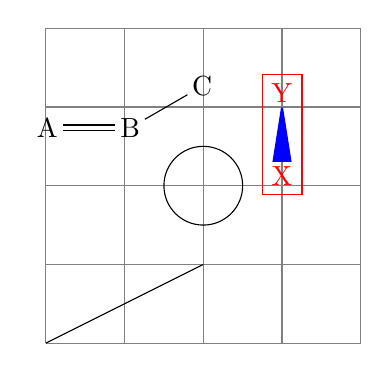
\begin{tikzpicture}[help lines/.style={thin,draw=black!50}]
		\draw[help lines] (0,0) grid (4,4);
		\draw(0,0) -- (2,1);
		\draw(2,2) circle (0.5);
		\node at (1,3) {\chemfig{A=B-[:30]C}};
		\node[draw,red,anchor=base] at(3,2){\chemfig{X>[2,,,,blue]Y}};
	\end{tikzpicture}|

\section{Beyond chemistry}\label{style.noeuds}
At heart \CF is a tool for drawing graphs, and this tool has been programmed to adapt it for chemistry. In some ways it is possible to return \CF to its roots to draw organization charts or other diagrams represented by graphs.

Each atom is contained in a \TIKZ node. By default these nodes have an ``inner sep'' and an ``outer sep'' equal to 0pt. They are rectangular as seen on page~\pageref{longueur.liaison}. These defaults can be overwritten with the macro \idx{\setnodestyle}, the argument of which is passed to \TIKZ and specifies the style of the nodes containing the atoms.

In this example we specify only ``draw,inner sep=2pt'', which has the effect of drawing the outline of the nodes and separating the outline and node contents by 2pt. We also specify \verb-\setbondoffset{0pt}-\idx{\setbondoffset} so that the bonds touch the edges of the nodes. The interatomic spacing is increased to 75pt. Finally, the command \idx{\printatom} is made as simple as possible so that math mode is no longer used and spaces are thus preserved.
\exemple*{An organization chart}/\setnodestyle{draw,inner sep=2pt}
\setbondoffset{0pt}
\setatomsep{75pt}
\renewcommand\printatom[1]{#1}
\chemfig{The boss-[6]Me(-[4]Them(-[6]The others)(-[7,2]Group 1))-You(-[:-120,0.5]Him)(-[:-60,0.5]Her)}/

Here is another organization chart where the nodes are circular and coloured cyan\idx*{\printatom}:
\exemple*{Family diagram}/\setnodestyle{draw,circle,fill=cyan,minimum size=30pt}
\setbondoffset{0pt}
\setatomsep{80pt}
\renewcommand\printatom[1]{\textsf{#1}}
\chemfig{Me(-[:-50,1.2]Brother)(-[:-10]Brother(-[:15]Niece)(-[:-35]Niece))
(-[:-155,0.8]Sister-[:-80]Nephew)(-[:95,1.25]Father(-[:-25,0.8]Uncle)(-[:-65,0.8]Aunt))
(-[:135]Mother-[:-95,0.5]Uncle)}/

\section{Annotated examples}\label{exemples.commentes}
In this chapter, several molecules will be drawn, putting into use the methods previously described. The aim here is to show a logical order for putting together a molecule so that the user unfamiliar with \CF will learn how to construct complex molecules. The construction steps will be shown to help with this learning process.

In addition, several possibilities --- some intuitive and others less so --- will be shown which give the same graphical results, with the objective being to show that \CF allows some flexibility in encoding molecules. One can see how each is put together and adopt the methods with which one is most comfortable.

\subsection{Ethanal}
Here we will draw the ethanal (or acetaldehyde) molecule: \chemfig{H-C(-[2]H)(-[6]H)-C(-[7]H)=[1]O}

The best method for non-cyclic molecules is to select the longest chain. Here one could take ``\verb|H-C-C=0|'' for example. The bond \verb|C=O| is tilted to 45\degres{} by using the predefined angle ``\verb-[1]-''. This give a ``backbone'' of the molecule to which the branches merely have to be added\idx*{bond!angle!predefined}:
\exemple{Backbone of ethanal}|\chemfig{H-C-C=[1]O}|

The three hydrogen atoms still have to placed at the correct orientation with the help of predefined angles. The first is at 90\degres{} with the branch\idx*{bond!branch} ``\verb/(-[2]H)/'', the second at 270\degres{} with ``\verb/(-[6H])/'', and the one on the right at 315\degres{} with ``\verb/(-[7]H)/'':
\exemple{Ethanal}|\chemfig{H-C(-[2]H)(-[6]H)-C(-[7]H)=[1]O}|

\subsection{2-amino-4-oxohexanoic acid}
Here is the molecule to be drawn: \chemfig{-[::+30]-[::-60](=[:-90]O)-[::+60]-[::-60](-[:-90]NH_2)-[::+60](=[:90]O)-[::-60]OH}

As is often the case for most molecules, there are several methods and for each several different ways of getting the result. Here we will look at four different methods.

\subsubsection{Absolute angles}
\idx*{bond!angle!absolute}We will first of all draw the central chain with absolute angles. We set the default angle to $+30\degres$ with the optional argument\idx*{chemfig@\protect\texttt{\protect\string\protect\chemfig}!optional arguments}, and so only the descending bonds need to have their absolute angle set to $-30\degres$:
\exemple{Backbone (absolute angles)}|\chemfig{[:30]--[:-30]--[:-30]--[:-30]OH}|

The branches\idx*{bond!branch} ``\verb/(=[6]O)/'', ``\verb/(-[6]NH_2)/'' and ``\verb/(=[2]O)/'' still have to be added to the correct vertices:
\exemple{Molecule (absolute angles)}|\chemfig{[:30]--[:-30](=[6]O)--[:-30](-[6]NH_2)-(=[2]O)-[:-30]OH}|

\subsubsection{Relative angles}
\idx*{bond!angle!relative}A more general approach uses only relative angles, in this way:
\exemple{Structure (relative angles)}|\chemfig{[:30]--[::-60]--[::-60]--[::-60]OH}|

then
\exemple{Molecule (relative angles)}|\chemfig{[:30]--[::-60](=[::-60]O)--[::-60](-[::-60]NH_2)
-(=[::60]O)-[::-60]OH}|

\subsubsection{Ring}
Since the angles between the bonds are 120\degres{}, it is possible to use a 6-ring, although this method is less natural. Here we take advantage of the fact that a ring can be left unfinished\idx*{ring!unfinished}. The ring must be rotated 120\degres{} so that the first vertex is to the south-east of the ring:
\exemple{Backbone (ring)}|\chemfig{[:120]NH_2*6(---=O)}|

\idx*{ring!branch}Now the branches must be added to the right vertices:
\exemple{Molecule (ring)}|\chemfig{[:120]NH_2*6(-(-(=[::60]O)-[::-60]OH)--(--[::60])=O)}|

\subsubsection{Nested rings}
\idx*{ring!nested}Delving deeper into the ring method, we can also consider nesting incomplete 6-rings. We could start with this backbone:
\exemple{Backbone (nested rings)}|\chemfig{*6(--*6(--=O))}|

And then add the bonds which leave the vertices of these rings. There are no angles to worry about because the bonds leaving the rings are the bisectors of the sides of the ring, exactly what we want here:
\exemple{Molecule (nested rings)}|\chemfig{*6((-)-(=O)-*6(-(-NH_2)-(-OH)=O))}|

A close look shows that the second line segment of the double bond to the oxygen atom is \emph{inside} the incomplete 6-ring\footnote{This was also true for the preceding method with one ring.} Despite its brevity, this code does not give a perfect drawing. This can of course be corrected by adding a little to the code:
\exemple{Molecule (corrected nested rings)}|\chemfig{*6((-)-(=O)-*6(-(-NH_2)-(-OH)(=[::60]O)))}|

\subsection{Glucose}
The goal here is to represent the glucose molecule according to several different conventions.

\subsubsection{Skeleton diagram}
\idx*{skeleton diagram}The code here looks like that of 2-amino-4-oxohexanoic acid. This gives almost the same structure with absolute angles, except here the default angle is $-30\degres$:
\exemple[60]{Backbone}|\chemfig{[:-30]HO--[:30]--[:30]--[:30]-H}|

Adding the branches is no problem. We use predefined absolute angles:
\exemple[60]{Glucose, skeleton diagram}|\chemfig{[:-30]HO--[:30](<[2]OH)-(<:[6]OH)
-[:30](<:[2]OH)-(<:[6]OH)-[:30](=[2]O)-H}|

\subsubsection{Fisher projection}
\idx*{Fisher projection}The goal is to get the molecule below:
\begin{center}
	\definesubmol{x}{(-[4]H)(-[0]OH)}
	\definesubmol{y}{(-[0]H)(-[4]OH)}
	\chemfig{[2]OH-[3]-!x-!x-!y-!x-=[1]O}
\end{center}
The idea is to begin to draw the longest chain vertically by giving a default angle of ``\verb-[2]-''. Here is the skeleton, where we have added lower case letters at the end of each vertical bond:
\exemple{Skeleton}|\chemfig{[2]OH-[3]-a-b-c-d-=[1]O}|

Next we define two aliases for the horizontal bonds and the atoms at their ends. Lets choose ``\verb-x-'' which we will put in place of the lower case a, c and d, and ``\verb-y-'' which will replace the letter c. Since these alias are just one character, we do not need braces and can write ``\verb-!x-'' instead of ``\verb-!{x}-''\idx*{\definesubmol}:
\exemple{Glucose (Fisher projection)}|\definesubmol{x}{(-[4]H)(-[0]OH)}
\definesubmol{y}{(-[0]H)(-[4]OH)}
\chemfig{[2]OH-[3]-!x-!x-!y-!x-=[1]O}|

\subsubsection{``Chair'' representation}
\idx*{chair representation}We will depict the $\alpha$-D-glucose molecule:
\chemfig{?(-[:190]OH)-[:-50](-[:170]OH)-[:10](-[:-55,0.7]OH)-[:-10](-[6,0.7]OH)-[:130]O-[:190]?(-[:150,0.7]-[2,0.7]OH)}

To do this, we will first of all draw five sides of the chair and link the first vertex to the last with a hook ``\verb-?-''. We will use the following absolute angles, running counterclockwise: $-50\degres$, $10\degres$, $-10\degres$, $130\degres$, $190\degres$.
\exemple{Structure}|
\chemfig{?-[:-50]-[:10]-[:-10]-[:130]O-[:190]?}|

Now we simply add the branches inside parentheses. The angles are chosen to give the best impression of perspective, and some bonds are shortened by a factor of 0.7:
\exemple{Chair representation}|\chemfig{?(-[:190]OH)-[:-50](-[:170]OH)-[:10](-[:-55,0.7]OH)
-[:-10](-[6,0.7]OH)-[:130]O-[:190]?(-[:150,0.7]-[2,0.7]OH)}|

\subsubsection{Haworth projection}
\idx*{Haworth projection}The goal is to depict this D-glucopyranose molecule:
{\setcrambond{2pt}{}{}
\chemfig{HO-[2,0.5,2]?<[7,0.7](-[2,0.5]OH)-[,,,,line width=2pt](-[6,0.5]OH)>[1,0.7](-[6,0.5]OH)-[3,0.7]O-[4]?(-[2,0.3]-[3,0.5]OH)}}

First of all we will choose the longest chain, which starts at the ``HO'' group on the left and continues through fives sides of the ring. The ring will be closed with a hook. For the vertical bond which leaves from the first ``HO'' group, we need to specify that it will leave from the second atom using the optional argument. Furthermore, it will be shortened with a coefficient of 0.5. Its optional argument\idx*{chemfig@\protect\texttt{\protect\string\protect\chemfig}!optional arguments} will thus be ``\verb/[2,0.5,2]/''.

Next, to give the impression of perspective to the ring, the diagonal bonds will be shortened by a coefficient of 0.7. For the bold diagonal lines we will use Cram bonds, having redefined the base of the triangles to be 2pt. The bold horizontal bond needs to be drawn with a thickness of 2pt, and so its optional argument will be ``\verb/[0,,,,line width=2pt]/''. Here is the skeleton of the molecule\idx*{\setcrambond}:
\exemple{Structure}|\setcrambond{2pt}{}{}
\chemfig{HO-[2,0.5,2]?<[7,0.7]-[,,,,
line width=2pt]>[1,0.7]-[3,0.7]O-[4]?}|

All that needs to be done now is to add the branches at the correct places, giving the right absolute angles and sometimes reducing the length to better give the illusion of perspective\idx*{\setcrambond}:
\exemple{Haworth projection}|\setcrambond{2pt}{}{}
\chemfig{HO-[2,0.5,2]?<[7,0.7](-[2,0.5]OH)-[,,,,
line width=2pt](-[6,0.5]OH)>[1,0.7](-[6,0.5]OH)-[3,0.7]
O-[4]?(-[2,0.3]-[3,0.5]OH)}|

\subsection{Adrenaline}
We want to draw the adrenaline molecule:
\chemfig{*6((-HO)-=-(-(<[::60]OH)-[::-60]-[::-60,,,2]HN-[::+60]CH_3)=-(-HO)=)}

We are going to use two different methods.

\subsubsection{Using one ring}
First of all, we start with a 6-ring and we draw the start of the branches\idx*{ring!branch} which leave it:
\exemple[60]{Skeleton of adrenaline}|\chemfig{*6((-HO)-=-(-)=-(-HO)=)}|

The branch on the right still needs to be completed using, for example, relative angles:
\exemple[60]{Adrenaline, step two}|\chemfig{*6((-HO)-=-(--[::-60]-[::-60]
HN-[::+60]CH_3)=-(-HO)=)}|

Then we need to add a Cram-bonded \verb-OH- and indicate that the bond which arrives at ``\verb-HN-'' does so on the second atom, i.e., ``N''. We use the fourth optional argument of the bond\idx*{chemfig@\protect\texttt{\protect\string\protect\chemfig}!optional arguments}:
\exemple[60]{Adrenaline}|\chemfig{*6((-HO)-=-(-(<[::60]OH)-[::-60]-[::-60,,,2]
HN-[::+60]CH_3)=-(-HO)=)}|

\subsubsection{Using two rings}
This method is less natural, but the goal is to show here how to make a bond invisible\idx*{bond!invisible}.

We could improve this code by considering that the drawing of the adrenaline molecule is made of two 6-rings adjacent\idx*{ring!nested} to each other:
\exemple[60]{Adrenaline, two-ring skeleton}|\chemfig{*6((-HO)-=*6(--HN---)-=-(-HO)=)}|

Now the first two bonds of the ring on the right need to be made invisible. To do this we use the argument that is passed to \TIKZ, specifying ``\verb-draw=none-''. These bonds will thus have this code: ``\verb/-[,,,,,draw=none]/''. To keep the code readable, we define an alias named ``\verb-&-'' for these bonds\idx*{\definesubmol}:
\exemple[60]{Adrenaline, step two}|\definesubmol{&}{-[,,,,draw=none]}
\chemfig{*6((-HO)-=*6(!&!&HN---)-=-(-HO)=)}|

The rest becomes easy; just add the branches to the right vertices\idx*{\definesubmol}:
\exemple[60]{Adrenaline, step three}|\definesubmol{&}{-[,,,,draw=none]}
\chemfig{*6((-HO)-=*6(!&!&HN(-CH_3)--(<OH)-)-=-(-HO)=)}|

To finish, we specify that the bonds that \emph{arrive at and leave from} ``\verb-HN-'' must do so at the second atom. We therefore define another alias for the invisible bond which arrives at ``\verb-HN-''\idx*{\definesubmol}:
\exemple[60]{Adrenaline}|\definesubmol{&}{-[,,,,draw=none]}
\definesubmol{&&}{-[,,,2,draw=none]}
\chemfig{*6((-HO)-=*6(!&!{&&}HN(-CH_3)-[,,2]-(<OH)-)-=-(-HO)=)}|

\subsection{Guanine}
We will draw the guanine molecule:
\chemfig{*6((-H_2N)=N-*6(-\chembelow{N}{H}-=N?)=?-(=O)-HN-[,,2])}\medskip

First of all, let's begin by drawing the nested rings\idx*{ring!nested}, putting just the nitrogen atoms at the vertices:
\exemple{Guanine, skeleton}|\chemfig{*6(=N-*6(-N-=N)=--N-)}|

Then we can draw the horizontal bond in the right ring with a hook. We will also place a hydrogen atom under the nitrogen atom of the 5-ring with the command \verb-\chembelow{N}{H}-. We also need to write ``\verb-HN-'' instead of ``\verb-N-'' at the vertex at the upper left of the molecule\idx*{\chembelow}:
\exemple{Guanine, step two}|\chemfig{*6(=N-*6(-\chembelow{N}{H}-=N?)=?--HN-)}|

We note that one bond leaves from the wrong atom\footnote{This seems illogical because the angle of the bond from the \texttt{HN} group toward the first vertex lies between $-90\degres$ and $90\degres$; \CF should therefore leave from the second atom. To explain this contradiction, one must know that in rings, the last bond always links the last vertex to the first, ignoring the \emph{calculated theoretical} angle of this bond (which here is $-90\degres$). \CF uses this theoretical angle to determine the departure and arrival atoms, but does not use it to draw the bond because the two ends are already defined. The departure atom for the last bond is thus the first atom.}! The automatic calculation mechanism must be corrected so that the bond leaves from the second atom ``\verb-N-'' instead of the first. To do this we give an optional argument for the last bond of the first 6-ring ``\verb-[,,2]-'':
\exemple{Guanine, step three}|\chemfig{*6(=N-*6(-\chembelow{N}{H}-=N?)=?--HN-[,,2])}|

Simply add the branches to the right vertices. Note especially the branch leaving the first vertex of the first 6-ring ``\verb/(-N_2N)/'':
\exemple{Guanine}|\chemfig{*6((-H_2N)=N-*6(-\chembelow{N}{H}-=N?)=?-(=O)-HN-[,,2])}|

We could also draw the same molecule with a regular 5-ring, as is sometimes done:
\exemple{Guanine with 5-ring}|\chemfig{*6((-H_2N)=N-*5(-\chembelow{N}{H}-=N-)=-(=O)-HN-[,,2])}|

\section{How to \protect\ldots}
\subsection{Write a colored atom}
\idx*{color (atom)}Since the package \verb-xcolor- is loaded by \TIKZ, itself loaded by \CF, we can write color commands in the code of a molecule, mainly \idx{\color} and \idx\textcolor. The atoms are displayed in \TIKZ nodes which behaves like boxes of \TeX{} and it is as if these atoms were put in a group. Therefore, the color change remains local to the atom.

\exemple{Colors}/\chemfig{C\color{blue}H_3-C(=[1]O)-[7]O\color{red}H}/

This code does not work, because of the rule used to separate atoms\idx*{separating atom mechanism}: here, the first atom sarts at ``\verb-C-'' and spreads to the next uppercase letter. Therefore, this atom is ``\verb-C\color{blue}-'' and the color change occurs at the end of atom and has no effect. We need to force \CF to cut the first atom just after ``\verb-C-'' with the character ``\verb-|-'' and then include \verb-\color{blue}H_3- between braces so that \CF does not stop the atom 2 before the uppercase ``\verb-H-'' which would leave the color change alone and therefore ineffective in an atom:

\exemple{Colors}/\chemfig{C|{\color{blue}H_3}-C(=[1]O)-[7]O|{\color{red}H}}/

The same effect can be obtained with \verb-\textcolor-:

\exemple{Colors}/\chemfig{C|\textcolor{blue}{H_3}-C(=[1]O)-[7]O|\textcolor{red}{H}}/

The main disadvantage is that we have to do the same for every atom that need to be colored, even if they are contiguous.

\subsection{Add a superscript without modifying a bond}
Adding a \idx{charge} to an atom with a mathematical exponent implies that the box (and therefore the \TIKZ node) containing the atom has its dimensions modified. It has no importance when the atom is trailing but the alignment may be compromised if a bond is attached to the atom. The first reaction is to put the charge in a box with no width and therefore use the command \idx\rlap\footnote{If you have to put the charge at the left of the atom, you must use the command \texttt{\string\llap.}}, which often gives good results. We see here that with \idx\rlap, the \idx{horizontal alignment} of atoms is preserved:
\exemple{Charge and bond}/\chemfig{A^+-[2]B}
\qquad
\chemfig{A\rlap{${}^+$}-[2]B}/
If you want to use the command \verb-\oplus- which displays ``$\oplus$''\idx*{charge!\protect\texttt{\protect\string\protect\oplus}}, some could find that the charge is too low: $\mathrm{A^\oplus}$. In that case, why not use \idx{\chemabove} to put as precisely as you will, both vertically and horizontally the charge:
\exemple{Charge et \string\chemabove}/\chemfig{\chemabove[0.5pt]{A}{\scriptstyle\hspace{3.5mm}\oplus}-[2]B}
\qquad
\chemfig{{\chemabove[-0.5pt]{A}{\scriptstyle\hspace{3.5mm}\oplus}}-[2]B}/
We notice an additional level of braces for the second molecule. Indeed, as we specify ``\verb/-0.5pt/'' for the optional argument of \idx{\chemabove} to lower the charge, it is necessary to prevent \CF to understand the sign ``\verb/-/'' as a single bond.

To add a load near the vertex of a cycle \idx*{charge}, the best method is to attach an invisible bond \idx*{bond!invisible} to this vertex, which is done here with \idx{\definesubmol} with a bond with a length coefficient equal to 0.2:
\exemple{Charges and cycles}/\definesubmol\nobond{-[,0.2,,,draw=none]}
\chemfig{*5(---(!\nobond\scriptstyle\oplus)-(!\nobond\scriptstyle{-})-)}/

\subsection{Draw a curve bond}
We have already seen that with the \TIKZ library ``\verb-decorations.pathmorphing-'', we can draw a wavy bond\idx*{bond!wavy}:

\exemple{Wavy bond}|\chemfig{A-[,3,,,decorate,decoration=snake]B}

\chemfig{A-[,3,,,decorate,decoration={snake,amplitude=1.5mm,
    segment length=2.5mm}]B}|

For more flexibility, you can also define nodes using the character ``\verb-@-''\idx*{"@} and reuse these nodes after the molecule has been drawn to connect them with a curved line using \idx\chemmove:

\exemple{Curved bonds}/\chemfig{@{a}A-[,,,,draw=none]@{b}B}
\chemmove{\draw[-](a)..controls +(45:7mm) and +(225:7mm)..(b);}
\bigskip

\chemfig{*6(@{a}---@{b}---)}
\chemmove{\draw[-](a)..controls +(60:3em) and +(240:3em)..(b);}
\quad
\chemfig{*6(@{a}---@{b}---)}
\chemmove{\draw[-](a)..controls +(60:3em) and +(30:1em)..
    ++(20:2em) ..controls +(210:3em) and +(-120:4em) ..(b);}/

\subsection{Modify the size of a molecule}
\idx*{size of molecules}Two parameters determine the default size of a molecule: the font size and the parameter of \idx{\setatomsep} which is 3em the default. We can modify independently these two parameters to change the size of a molecule:

\exemple{Change the size}/\definesubmol\hho{H-[:30]O-[:-30]H}
\chemfig{!\hho}

\setatomsep{2.5em}\chemfig{!\hho}

\scriptsize\chemfig{!\hho}

\tiny\chemfig{!\hho}\setatomsep{5em}\chemfig{!\hho}/

You can use the optional second argument of \verb-\chemfig-\idx*{chemfig@\protect\texttt{\protect\string\protect\chemfig}!optional arguments} to \emph{globally} enlarge or reduce a molecule, i.e. the text and links will be reduced by the same ratio:

\exemple{Global change of the size}/\definesubmol\hho{H-[:30]O-[:-30]H}
\chemfig{!\hho}

\chemfig[][scale=0.75]{!\hho}

\chemfig[][scale=0.5]{!\hho}

\chemfig[][scale=0.33]{!\hho}/

\subsection{Draw a ploymer element}
\idx*{polymer}The difficulty lies in the display of delimiters (parentheses or brackets) on bond. For this, we will again use the character ``\verb-@-''\idx*{"@} to define global nodes that will be used later as anchors for delimiters.

We will write a simple macro \verb-\setpolymerbracket-, followed by two characters which define the opening delimiter and closing delimiter.

Then, the macro \verb-\makebraces- has an argument of the form ``\verb-[<dim up>,<dim down>]-''. These two dimensions are the height and depth of the delimiters from the baseline. The following arguments are the subscript located at the right bottom of the closing delimiter and the names of the 2 nodes at which the opening and closing delimiters will be drawn.

\exemple*{Polymers}|\newcommand\setpolymerdelim[2]{\def\delimleft{#1}\def\delimright{#2}}
\def\makebraces[#1,#2]#3#4#5{%
	\edef\delimhalfdim{\the\dimexpr(#1+#2)/2}%
	\edef\delimvshift{\the\dimexpr(#1-#2)/2}%
	\chemmove{%
		\node[at=(#4),yshift=(\delimvshift)]
			{$\left\delimleft\vrule height\delimhalfdim depth\delimhalfdim
			width0pt\right.$};%
		\node[at=(#5),yshift=(\delimvshift)]
			{$\left.\vrule height\delimhalfdim depth\delimhalfdim
			width0pt\right\delimright_{\rlap{$\scriptstyle#3$}}$};}}
\setpolymerdelim()
Polyéthylène:
\chemfig{\vphantom{CH_2}-[@{op,.75}]CH_2-CH_2-[@{cl,0.25}]}
\makebraces[5pt,5pt]{\!\!n}{op}{cl}
\bigskip

Polyvinyl chloride:
\chemfig{\vphantom{CH_2}-[@{op,.75}]CH_2-CH(-[6]Cl)-[@{cl,0.25}]}
\makebraces[5pt,25pt]{\!\!\!n}{op}{cl}
\bigskip

Nylon 6:
\chemfig{\phantom{N}-[@{op,.75}]{N}(-[2]H)-C(=[2]O)-{(}CH_2{)_5}-[@{cl,0.25}]}
\makebraces[30pt,5pt]{}{op}{cl}
\bigskip

Polycaprolactame:\setatomsep{2em}
\chemfig{[:-30]-[@{left,.75}]N(-[6]H)-[:30](=[2]O)--[:30]--[:30]--[@{right,0.25}:30]}
\makebraces[5pt,25pt]{\!\!\!n}{left}{right}
\bigskip

\setpolymerdelim[]
Polyphénylène sulfide:
\chemfig{\vphantom{S}-[@{op,.75}]S-(**6(---(-[@{cl,0.25}])---))}
\makebraces[15pt,15pt]{}{op}{cl}
\bigskip

\chemfig{-CH_2-CH([6]-CO-NH-CH_2-NH-CO-CH([4]-CH_2-)([0]-[@{downleft,0.8},2]CH_2
-CH([2]-CO-NH_2)-[@{downright,0.3},2]CH_2-[,1.5]C?H-))-[@{upleft,0.8},2]CH_2
-CH([6]-CO-NH_2)-[@{upright,0.3},2]CH_2-[,1.5]CH([6]-CO-NH-CH_2-NH-C?O)-}
\makebraces[5pt,40pt]{n}{upleft}{upright}
\makebraces[38pt,7pt]{n}{downleft}{downright}|

\subsection{Draw the symmetrical of a molecule}\label{retournement}
\idx*{symmetrical of a molecule}The two commands \idx{\hflipnext} and \idx{\vflipnext} allow to draw the symmetrical of the next molecule about a horizontal or vertical axis. If we want to draw more symmetrical molecules, we need to write these commands before each molecule involved.

\exemple{Symmetry}/\chemfig{H_3C-C(=[:30]O)-[:-30]OH}% original

\vflipnext
\chemfig{H_3C-C(=[:30]O)-[:-30]OH}\medskip

\chemfig{H_3C-C(=[:30]O)-[:-30]OH}% original
\hflipnext
\chemfig{H_3C-C(=[:30]O)-[:-30]OH}/

\subsection{Add text above bonds and arc to angles}
\idx*{bond!with text}Once we have understood that the character ``\verb-@-''\idx*{"@} can put a ``global'' \TIKZ node, that is to say a node accessible after the molecule has been drawn, everything that \TIKZ can do with nodes (that is to say a lot of things) becomes possible.

To write something above or below a bond, we can put two ``global'' nodes on the atoms at the ends of this bond and write midway of them a text, raised or lowered so that it falls to just above or below the bond. This is done by the macro \verb-\bondname- in the code below \footnote{The \texttt{\string\si} command is provided by the \href{http://www.ctan.org / tex-archive/help/Catalogue/entries/siunitx.html}{\texttt{\textbf{siunitx }}} package.}.

\idx*{bond!angle!arc}To draw an arc between two bonds, three atoms are involved on which we have to put three ``global'' nodes. The macro  \verb-\arcbetweennodes- calculates the angle between two lines drawn from a node. Then \verb-\arclabel- draws an arc between two bonds and writes a text next to the arc: the optional argument of this macro is the \TIKZ code used to custom the arc. The second argument is the radius of the arc and the following three arguments are the names of global nodes between which the arc must be drawn, the middle name needs to be the vertex of the angle. The last argument is the text to write.

\exemple*{Arcs and text on bonds}|
\newcommand\namebond[4][5pt]{\chemmove{\path(#2)--(#3)node[midway,sloped,yshift=#1]{#4};}}

\newcommand\arcbetweennodes[3]{%
  \pgfmathanglebetweenpoints{\pgfpointanchor{#1}{center}}{\pgfpointanchor{#2}{center}}%
  \let#3\pgfmathresult}

\newcommand\arclabel[6][stealth-stealth,shorten <=1pt,shorten >=1pt]{%
  \chemmove{%
    \arcbetweennodes{#4}{#3}\anglestart \arcbetweennodes{#4}{#5}\angleend
    \draw[#1]([shift=(\anglestart:#2)]#4)arc(\anglestart:\angleend:#2);
    \pgfmathparse{(\anglestart+\angleend)/2}\let\anglestart\pgfmathresult
    \node[shift=(\anglestart:#2+1pt)#4,anchor=\anglestart+180,rotate=\anglestart+90,inner sep=0pt,
          outer sep=0pt]at(#4){#6};}}

\chemfig{@{a}A=[:30,1.5]@{b}B-[7,2]@{c}C-@{d}D}
\namebond{a}{b}{\scriptsize My text}
\namebond[-3.5pt]{b}{c}{\small\color{red}$\pi$}
\namebond{c}{d}{\small1\si\angstrom}
\medskip

Horizontal water molecule: \chemfig{@{1}H-[::37.775,2]@{2}O-[::-75.55,2]@{3}H}.
\namebond{1}{2}{\footnotesize0.9584\si\angstrom}
\namebond{2}{3}{\footnotesize0.9584\si\angstrom}
\arclabel{0.5cm}{1}{2}{3}{\footnotesize104.45\si\degree}
\qquad
Water molecule rorated 30\si\degree: \chemfig{[:30]@1H-[::37.775,2]@2O-[::-75.55,2]@3H}
\namebond12{\footnotesize0.9584\si\angstrom}
\namebond23{\footnotesize0.9584\si\angstrom}
\arclabel{0.5cm}{1}{2}{3}{\footnotesize104.45\si\degree}|
\newpage

\part{Reaction schemes}\label{schemas}
\idx*{reaction scheme|(}Following several requests from users, it had become evident that \CF had a weakness regarding the drawing of reaction schemes. The gap is now filled. Therefore, \CF has now reached version 1.0 since I consider that the main features sought are now available.

I thank Clemens \textsc {Niederberger} for his help and the tests he carried out on the new features presented in this part.
\section{Overview}\label{schemestart}
A reaction scheme must be contained between the commands ``\idx\schemestart'' and ``\idx\schemestop''. As shown in this example, \idx{debug information} is either hidden or displayed  with the command ``\idx\schemedebug'' and the argument ``false'' or ``true'':
\exemple[50]{Example 1}/\schemedebug{false}
\schemestart
  \chemfig{*6(-=-=-=)}\arrow
  \chemfig{X=[1]Y}\arrow
  \chemfig{S>T}
\schemestop
\bigskip

\schemedebug{true}
\schemestart
  \chemfig{*6(-=-=-=)}\arrow
  \chemfig{X=[1]Y}\arrow
  \chemfig{S>T}
\schemestop/

Some comments:
\begin{itemize}
	\item the \idx{\arrow} commands draw the arrows;
	\item everything lying between two \idx{\arrow} commands is considered a \idx{compound}. It was decided that all possible settings, whether for arrows or compounds, are controlled by the arguments of the \idx{\arrow} command, whose syntax may become quite complex;
	\item arrows are plotted horizontally, this can obviously be modified;
	\item  arrows are plotted on the imaginary line connecting the center of the compounds' bounding boxes  (the red and blue squares are the anchoring points of arrows). This behavior can also be modified;
	\item debug information is displayed with the \idx{\schemedebug} command. It consists of:
	\begin{itemize}
		\item the green label above the bounding boxes is the default name assigned to compounds by \CF. It follows the series "c1", "c2", etc. Numbering is reset to 1 for every reaction scheme.
		\item display of the compounds bounding boxes;
		\item the arrows start and end points represented by red points and anchors by blue points;
	\end{itemize}
	\item the distance from edge to edge between two compounds is defined with the \idx*\setcompoundsep\verb-\setcompoundsep{<dim>}-\label{setcompoundsep} command, where the argument is a valid dimension in the sense of \TeX{}. By default, and if the argument is empty, this dimension is 5em;
	\item finally, the distance between the edges of the compounds and the beginning and end of the arrows is defined with the \idx*\setarrowoffset\verb-\setarrowoffset{<dim>} command- where the argument is valid under a dimension of \TeX{}. By default, and if the argument is empty, this dimension is 4pt.\label{setarrowoffset}
\end{itemize}

\section{Arrow types}\label{arrow}
When the \idx{\arrow} command is followed by an optional argument in braces (which is not mandatory), the argument defines the type of arrow\idx*{arrow!type}:
\exemple[50]{Arrow types}|\schemestart A\arrow{->}B\schemestop\par % by default
\schemestart A\arrow{-/>}B \schemestop\par
\schemestart A\arrow{<-}B \schemestop\par
\schemestart A\arrow{<->}B \schemestop\par
\schemestart A\arrow{<=>}B \schemestop\par
\schemestart A\arrow{<->>}B \schemestop\par
\schemestart A\arrow{<<->}B \schemestop\par
\schemestart A\arrow{0}B \schemestop\par
\schemestart A\arrow{-U>}B \schemestop|
The arrow ``\verb/-U>/'' is not fully drawn, an arc can be added tangent to the arrow center using  optional arguments on the command, see page~\pageref{fleche.arg.optionnel}. Here is a ``\verb/-U>/'' arrow with the arc on top of it: \schemestart A\arrow{-U>[$\scriptstyle x$][$\scriptstyle y$]}B\schemestop

For the sake of clarity, capital letters will be used throughout the documentation instead of chemical formulas made with the  \idx\chemfig command except for specific examples. Reaction schemes obviously work identically with letters and drawn molecules. Several examples are shown in the Gallery with proper reaction schemes.

\section{Arrows features}
Each \idx{arrow} is characterized by:
\begin{itemize}
	\item \idx*{arrow!angle}an angle expressed in degrees;
	\item \idx*{arrow!coefficient}a coefficient that specifies the arrow length through the multiplication of the compounds spacing value\idx*{compound!spacing} defined by \idx\setcompoundsep;
	\item \idx*{arrow!style} a style with \TIKZ instructions to customize the color, the thickness or other graphical attribute of the arrow.
\end{itemize}

These features are defined with the command \idx\setarrowdefault\verb-{angle,coeff,style}-\label{setarrowdefault}. And this is made \emph{outside} the reaction scheme. If the angle is empty, it takes the value 0, and if the coefficient is empty, it is equal to 1. The as-defined features will be kept throughout the document, from the point where the instruction is found. To reset the default settings, just enter an empty argument.
\exemple[50]{Definition of default values}/\schemestart A\arrow B\arrow C\schemestop

\setarrowdefault{15,1.5,red,thick}
\schemestart A\arrow B\arrow C\schemestop

\setarrowdefault{,2.5,dashed}
\schemestart A\arrow B\arrow C\schemestop

\setarrowdefault{}
\schemestart A\arrow B\arrow C\schemestop/

In order to locally modify one or all of these default values, the \idx{\schemestart} command accepts an optional argument in the form \verb-[angle,coeff,style]- which changes the default arrow features within the sole reaction scheme:
\exemple[50]{Optional argument}/\setarrowdefault{5,2.5,blue}
\schemestart A\arrow B\arrow C\schemestop

\schemestart[0] A\arrow B\arrow C\schemestop

\schemestart[0,1] A\arrow B\arrow C\schemestop

\schemestart[0,1,thick] A\arrow B\arrow C\schemestop

\schemestart[0,1,black] A\arrow B\arrow C\schemestop/
Regarding style\idx*{arrow!style}, the rule is: the style specified in the argument in brackets applies \emph{after} the default style, without overwrting it! This is why only the ``black'' color attribute is able to overwrite the `` blue'' default style.

Finally, the \idx{\arrow} command accepts an optional argument in brackets in  the form \verb-[angle,coeff,style]- to change the feature of that given arrow. As above, style applies \emph{after} the default style and \emph{after} the style possibly-specified in the optional argument of the \verb-\schemestart- command, again without overwrting them.
\exemple[50]{Arrows features}/\schemestart
  A\arrow[45]B\arrow[-20,2]C
\schemestop
\bigskip

\schemestart
  A\arrow[90,,thick]B\arrow[,2]C
  \arrow[-45,,dashed,red]D
\schemestop/

\section{Compounds names}
\idx*{compound!name}Automatic naming of compounds (``c1'', ``c2'', etc.) can be overridden. For this, the \idx{\arrow} command must be immediately followed by an argument in parentheses. The argument is of the form: \verb/(n1--n2)/. The compounds located at the beginning and at the end of the arrow are named ``\verb-n1-''  and ``\verb-n2-'', respectively. Any alphanumeric string can be used. The numbering of the names "c<n>" continues internally, so if a \idx{compound} has a different name than the default one, it does not affect the default name of the subsequent compounds.

Names are optional, and the argument can be either \verb/(n1--)/ and \verb/(--n2)/.

\exemple[50]{Compounds names}/\schemedebug{true}
\schemestart
  A\arrow(aa--bb)B\arrow(--cc)C\arrow(--dd)D\arrow E
\schemestop
\bigskip

\schemestart
  A\arrow(aa--)B\arrow(bb--)C\arrow(cc--dd)D\arrow E
\schemestop/
Note that both methods are equivalent. Therefore, compounds can either be named by arrows preceding or following them. However,  when a \idx{compound} is surrounded by two arrows specifying its name, the first name is ignored and a warning message is generated:
\exemple[50]{Overful naming}/\schemedebug{true}
\schemestart
  A\arrow(--foo)B\arrow(bar--)C
\schemestop/
Here \idx{compound} ``B'' is called ``foo'' by the arrow pointing at it, and ``bar'' by the arrowing leaving from it. Thus \CF generates a warning mentioning that the name "foo" will be ignored:

\hfill\verb-Package chemfig Warning: two names for the same node, first name "foo" ignored-\hfill\null

\section{Anchoring}
\idx*{compound!anchoring}As noted above, arrows lie on the line connecting the center of the compounds' bounding boxes. Default anchors are called ``center'' in the sense of \idx*{tikz}\TIKZ. Non-default anchoring points can be user-specified as well with an argument between brackets:

\hfill\verb/(n1.a1--n2.a2)/\hfill\null

where the anchor ``\verb-a1-'' or ``\verb-a2-'' can be: north west, north, north east, west, center, east, mid west, mid, mid east, base west, base, base east, south west, south , south east, text, or any angle. Here is an example from the \TIKZ  manual where the anchors are located on the bounding box:
\exemple*{TikZ anchoring}|\Huge
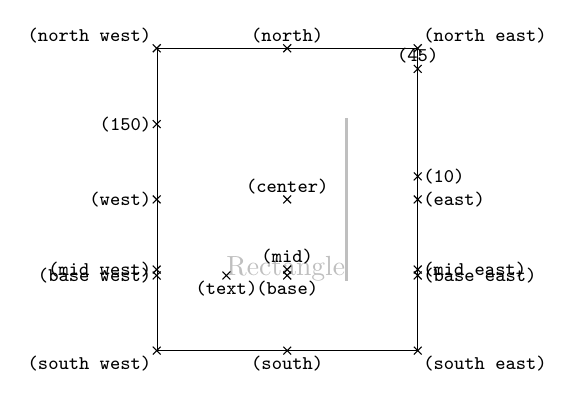
\begin{tikzpicture}[baseline]
\node[anchor=base west,name=x,draw,inner sep=25pt] {\color{lightgray}Rectangle\vrule width 1pt height 2cm};
\foreach \anchor/\placement in
{north west/above left, north/above, north east/above right,west/left, center/above, east/right,
mid west/left, mid/above, mid east/right,base west/left, base/below, base east/right,
south west/below left, south/below, south east/below right,text/below,10/right,45/above,150/left}
\draw[shift=(x.\anchor)] plot[mark=x] coordinates{(0,0)}
node[\placement,inner sep=0pt,outer sep=2pt] {\scriptsize\texttt{(\anchor)}};
\end{tikzpicture}|
Like for names, arrival and departure anchoring points are independent and optional.

In this example, the default alignment \idx*{reaction scheme!alignment} is not good because the two ``A'' are not aligned vertically.  Debug information\idx*{debug information} show that the default ``center'' anchors are not suitable:
\exemple[50]{Alignment problems}/\schemedebug{true}
\schemestart
  \chemfig{A*5(-----)}
  \arrow
  \chemfig{A*5(---(-)--)}
\schemestop/
For the alignment\idx*{reaction scheme!alignment} to be correct, arrows will leave/arrive either from the anchor ``base east''/``base west'', or from anchor  ``mid east''/``mid west'':
\exemple[50]{Alignment problems}/\schemedebug{true}
\schemestart
  \chemfig{A*5(-----)}
  \arrow(.base east--.base west)
  \chemfig{A*5(---(-)--)}
\schemestop
\bigskip

\schemestart
  \chemfig{A*5(-----)}
  \arrow(foo.mid east--bar.mid west)
  \chemfig{A*5(---(-)--)}
\schemestop/

\idx*{compound!anchoring}One last anchor need be specified: the anchor of the first \idx{compound} with respect to the \idx{baseline} of the text just before it. This is illustrated by the green point on the left-hand side of the scheme below:
\exemple[50]{Initial anchoring}/\schemedebug{true}
Preceding text:
\schemestart
  \chemfig{A*5(-----)}\arrow A
\schemestop/

The default position of this anchor on the first \idx{compound}'s bounding box is that given by  ``text''. This position can be controlled with the second optional argument of the \idx{\schemestart} command:
\exemple[50]{Adjusting the initial anchoring}/\schemedebug{true}
Preceding text:
\schemestart[][south]
  \chemfig{A*5(-----)}\arrow A
\schemestop
\bigskip

Preceding text:
\schemestart[][north west]
  \chemfig{A*5(-----)}\arrow A
\schemestop
\bigskip

Preceding text:
\schemestart[][west]
  \chemfig{A*5(-----)}\arrow A
\schemestop/

\section{Compounds style}
The \idx{\arrow} command can also include \TIKZ instructions to define the bounding box style ``\verb-s-'' of the reactant and the product of the reaction. This is done with the argument between parentheses. Always style through the argument in brackets of the \idx{\arrow}, we can specify with \TIKZ instructions the  style ``\verb-s-'' to bounding box of the \idx{compound}  of departure or of arrival. Therefore the complete syntax of the \idx{\arrow} command, with each specification being optional, is as follows:

\hfill\verb/\arrow(n1.a1[s1]--n2.a2[s2]){arrow type}[angle,coeff,arrow style]/\hfill\null

Like forn names, if  specific styles are given to one compound by arrows arriving on it and leaving from it, the first style will be ignored with a warning.

\exemple[60]{Compounds style}/\schemestart
  A
  \arrow([red]--[fill=blue,semitransparent,text opacity=1,
  inner sep=10pt,rounded corners=2mm])
  B
\schemestop
\bigskip

\schemestart
  A\arrow(--foo[yshift=5mm])B
\schemestop/
\label{setcompoundstyle}The macro \idx\setcompoundstyle\verb-{<code tikz>}- allows  to globally define the style of compounds \idx*{compound!style} displayed thereafter. Entering an empty argument results in the absence of style, which corresponds to the default case.

Here a style is defined with round corner-shaped boxes and semitransparent background:
\exemple[50]{Global styles}/\setcompoundstyle{draw,line width=0.8pt,semitransparent,
text opacity=1,inner sep=8pt,rounded corners=1mm}
\schemestart
  A\arrow([fill=red]--[fill=blue])[90]
  B\arrow(--[fill=gray])
  C\arrow(--[fill=green])[-90]
  D\arrow(--[draw=none])[-180]
\schemestop/

\section{Branching}
\idx*{reaction scheme!branching}So far, only linear reaction schemes have been treated. Branched schemes are also possible and this is where compound names play a key role. When a name is preceded by ``\verb-@-'' in the argument between brackets of the \idx{\arrow} command,  it means that the \idx{compound} already exists. Several scenarios are possible:
\begin{itemize}
	\item \verb/(@n1--n2)/: the arrow will leave from the existing compound ``\verb-n1-'' and the scheme will continue following the arrow, thus creating a branch;
	\item \verb/(@n1--@n2)/: the arrow is drawn between two existing compounds, no matter whether they are already defined or whether they will later in the reaction scheme: therefore this syntax can be placed \emph{anywhere} in the code of the reaction scheme;
	\item \verb/(n1--@n2)/: this syntax is not permitted;
\end{itemize}

In the following example, 3 branches are made, a first one from  ``B'', a second one from ``D'' and a last one from ``X''. Finally one more arrow connects two existing compounds: ``XX'' and ``D'':
\exemple[50]{Branching}/\schemestart
  A\arrow(aa--bb)B\arrow(--cc)C\arrow D
  \arrow(@bb--xx1)[-90]X\arrow[-90]Y% 1st branch
  \arrow(@c4--)[-90]Z\arrow W% 2nd branch
  \arrow(@xx1--xx2)[-45]XX% 3rd branch
  \arrow(@xx2--@c4)% XX-to-D arrow
\schemestop/

One may wish to have ``Y'' and ``XX'' on the same horizontal line. To achieve this, a horizontal invisible bond is drawn between ``Y'' and ``XX''; the scheme is completed with a final arrow between the two existing compounds ``XX'' and ``D'':
\exemple[50]{Branching}/\schemestart
  A\arrow(aa--bb)B\arrow(--cc)C\arrow D
  \arrow(@bb--xx1)[-90]X\arrow[-90]Y\arrow(--xx2){0}XX
  \arrow(@c4--)[-90]Z\arrow W
  \arrow(@xx1--@xx2)% X-to-XX arrow
  \arrow(@xx2--@c4)% XX-to-D arrow
\schemestop/

\section{Subscheme}\label{subscheme}
\idx*{reaction scheme!subscheme}A fraction of the reaction scheme can be defined within a single bounding box, so that \CF treats it as a \idx{compound}. The reaction scheme fraction is defined inside the compulsory argument between braces of the  \idx{\subscheme} command so it is subsequently reagarded as a single entity. When \idx{\subscheme} is located after an arrow, the command labels this subscheme as a \idx{compound} named ``c<n+1>'':
\exemple[50]{Subscheme}/\schemedebug{true}
\schemestart
  A\arrow
  \subscheme{B\arrow[-90,2]C}
  \arrow
  D
\schemestop/
Although this is not clearly seen because of labels overlap, the box around the subscheme is called ``c2'', and name numbering continues inside the subscheme with B called ``c3'' and C called  ``c4''. Since the first \idx{compound} in the subscheme is  ``B'', the subscheme's baseline is that of ``B''. This can be pointed out by specifying the anchors\idx*{reaction scheme!subscheme!anchoring}:
\exemple[50]{Subscheme}/\schemedebug{true}
\schemestart
  A\arrow(--.mid west)
  \subscheme{B\arrow[-90,2]C}
  \arrow
  D
\schemestop/
Note that since ``\idx\subscheme\verb-{<scheme>}-'' is only a convenient shortcut for \idx\schemestart\verb-<scheme>-\idx\schemestop, it can be used with the same optional arguments as \idx\schemestart.

\idx*{reaction scheme!subscheme!delimiter|(}\label{chemleft}\CF provides the \idx{\chemleft} and \idx{\chemright} command pair. These allow to set expandable delimiters on either side of a material. The commands must be followed by delimiters, just like in the case of \TeX{} primitive commands \verb-\left- and \verb-\right-:
\centerverb/\chemleft<car1><material>\chemright<car2>/
where \verb-<car1>- and \verb-<car2>- can be ``('' et ``)'' or ``['' and ``]'', or any other expandable delimiter consistent with the \verb-\left- et \verb-\right- commands.
\exemple{The \string\chemleft\ and \string\chemright macros}/\chemleft\lfloor\chemfig{A-[1]B}\chemright)

\chemleft\{\chemfig{A-[1,1.25]B-[6,1.25]C}\chemright|

\chemleft[\chemfig{H-[1]O-[7]H}\chemright]/
The code of the reaction scheme discussed above including \idx{\chemleft} and \idx{\chemright} is written:
\exemple{Reaction scheme with \string\chemleft\ and \string\chemright}/\schemestart
  A\arrow
  \chemleft[\subscheme{B\arrow[-90,2]C}\chemright]
  \arrow
  D
\schemestop/
\label{chemup}By analogy,  the macros \idx{\chemup} and \idx{\chemdown} can be used to draw expandable delimiters above and below the material, respectively:
\centerverb/\chemup<car1><material>\chemdown<car2>/
For example:
\exemple{The \string\chemup\ and \string\chemdown macros}/\schemestart[-90]
X\arrow
\chemup\{\chemfig{A-[1]B-[7]C}\chemdown\}
\arrow Y
\schemestop
\qquad
\schemestart[-90]
X\arrow
\chemup[\chemfig{A-[1]B-[7]C}\chemdown]
\arrow Y
\schemestop/

Delimiters can can also be drawn through compounds' style and apply them to a random compound (and hereby to a subscheme). These expandable delimiters (parentheses, brackets, braces) can be used upon loading the ``matrix'' \TIKZ library in the document preamble:

\hfill\verb-\usetikzlibrary{matrix}-\hfill\null

Since the  \idx{\chemleft}, \idx{\chemright}, \idx{\chemup} and \idx{\chemdown} commands are available, the  \CF package  will \emph{not} automatically load the library. As long as the user want to access this special set of delimiters, the library must be explicitly loaded.

The same brackets-delimited subscheme as above is presented again:
\exemple[50]{The ``matrix'' library delimiters}/\schemestart
  A\arrow(--[left delimiter={[}, right delimiter={]}])
  \subscheme{B\arrow[-90,2]C}
  \arrow
  D
\schemestop/
Since the delimiters are drawn outside the bounding box, it is advisable to slightly shorten the incoming and outgoing arrows:
\exemple[50]{Subscheme}/\schemestart
  A\arrow(--[left delimiter={[},
  right delimiter={]}])[,,shorten >=6pt]
  \subscheme{B\arrow[-90,2]C}
  \arrow[,,shorten <=6pt]
  D
\schemestop/\idx*{reaction scheme!subscheme!delimiter|)}

Subschemes should be used with care, undesired results are sometimes observed. In this example, a subscheme is used to horizontally align 3 different compounds:
\exemple[50]{Subscheme}/\schemedebug{true}
\schemestart
  A
  \arrow{0}[-90]
  \subscheme{%
    tagada\arrow{}
    tsoin\arrow{}
    fin}
  \arrow(xx--yy){}E
  \arrow(@c1--@c3){}
  \arrow(@c1--@c5){}
  \arrow(@c1--@c4){}
\schemestop/
The center of the subscheme is exactly located on the same vertical lign as the center of compound "A". This is because the two entities are connected by an  invisible arrow\idx*{arrow!invisible} with a $-90 $ angle. However, the arrow between the two pre-existing compounds ``A'' and ``tsoin'' is \emph{not}  vertical because ``tsoin'' is not on the center of the subscheme since "tagada" is wider than "end". If this arrow is to be vertical within the use of the \idx{\subscheme} command, one must find a correct angle  for the arrival anchor of the invisible arrow by try-and-error.

A much simpler method is to use a branch instead of a subscheme: draw a \emph{visible} arrow between ``A'' and ``tsoin'', and then draw horizontal arrows on both sides  of ``tsoin'', with a branch for the right-hand side arrows.
\exemple[50]{Subscheme}/\schemedebug{true}
\schemestart
  A
  \arrow(--tsoin){->}[-90]
  tsoin
  \arrow{<-}[180]
  tagada
  \arrow(@tsoin--fin){}
  fin
  \arrow{}
  E
  \arrow(@c1--@c3){}
  \arrow(@c1--@fin){}
\schemestop/

\section{Arrows optional arguments}\label{fleche.arg.optionnel}
\idx*{arrow!optional argument}Within the argument in braces of the \idx\arrow command, the arrow name can be followed by optional arguments written between brackets. Here are the possible values for these optional arguments and their meaning, as defined by \CF:
\begin{itemize}
	\item the arrows ``\verb|->|'', ``\verb|<-|'', ``\verb|<->|'', ``\verb|<=>|'', ``\verb|<<->|'',``\verb|<->>|'', ``\verb|-/>|'' have three optional arguments:
	\begin{itemize}
		\item the first one contains the ``label'' to be placed above the arrow\idx*{arrow!label};
		\item the second one contains the ``label'' to be placed below the arrow. The orientation of these two labels is given by the same angle as the arrow. The perpendicular shift\idx*{arrow!label!shift} between the arrow and the label anchor\idx*{arrow!label!anchoring} can be adjusted  with the \idx*\setarrowlabelsep\verb-\setarrowlabelsep{<dim>}-\label{setarrowlabelsep} command, its argument is a valid dimension in the sense of \TeX{}. By default or if the argument is empty, this distance is 3pt. Labels contained in the two optional arguments are \emph{not} typed in math mode.
		\item the third one is a dimension corresponding to a shift perpendicular to the arrow\idx*{arrow!shift} that can be applied to it: the dimension is positive for an upward shift of the arrow (and of its  labels, if any), and negative for a downward shift.
	\end{itemize}
	\item the ``\verb|-U>|'' arrow has 5 optional arguments:
	\begin{itemize}
		\item the first three are identical to those found in the other arrow types;
		\item the fourth one is a coefficient (which is 0.333 by default) which multiplies the length of the arrow to get the radius of the arc;
		\item the fifth one is the half-angle from the center of the arc path, it is 60 degrees by default.
	\end{itemize}
	\item the invisible arrow\idx*{arrow!invisible} ``\verb-0-'' accepts two optional arguments of the same type as the first two listed above;
\end{itemize}
\exemple[50]{Arrows optional arguments}/\schemedebug{false}
\schemestart A\arrow{->[up][down]}B \schemestop
\qquad
\schemestart A\arrow{->[up][down][4pt]}B \schemestop
\qquad
\schemestart A\arrow{->[up][down][-4pt]}B \schemestop
\medskip

\schemestart A\arrow{<=>[up][down]}[30,1.5]B \schemestop
\medskip

\schemestart[-20]
  A\arrow{->}B\arrow{->[][][3pt]}C\arrow{->[][][-3pt]}D
\schemestop/
A problem arises for vertical  arrows:
\exemple[50]{Vertical arrows}/\schemestart
  A\arrow{->[up][down]}[-90]B
\schemestop/
For the sake of clarity, one may prefer to have the ``above'' and ``below'' labels\idx*{arrow!label} written horizontally. Label angles\idx*{arrow!label!angle} can be specified, while default is the same angle as that of the arrow. To choose a specific angle, \verb-*{<angle>}- can be written at the beginning of the optional arguments:
\exemple[55]{Choice of angles}/\schemedebug{true}
\schemestart A\arrow{->[*{0}up][*{0}down]}[90]B\schemestop
\qquad
\schemestart A\arrow{->[*{0}up][*{0}down]}[45]B\schemestop
\qquad
\schemestart A\arrow{->[*{0}up][*{0}down]}[-45]B\schemestop
\qquad
\schemestart A\arrow{->[*{0}up][*{0}down]}[-90]B\schemestop/
The default position of the label anchor can lead to undesired results:
\exemple[50]{Anchors}/\schemedebug{true}
\schemestart
  A\arrow{->[*{0}on top of][*{0}underneath]}[45,2]B
\schemestop/
To counter this, the anchoring position\idx*{arrow!label!anchoring} can be specified as well to override the one selected by \CF by default. The syntax for this is: \verb-*{<angle>.<ancre>}-.
\exemple[50]{Anchors}/\schemedebug{true}
\schemestart
  A\arrow{->[*{0.0}on top of][*{0.180}underneath]}[45,2]B
\schemestop
\qquad
\schemestart
  A\arrow{->[*{0.south east}on top of]%
    [*{0.north west}underneath]}[45,2]B
\schemestop/

The ``\verb/-U>/'' arrow remains a particular case. If one of the two labels from the first two optional arguments is present, the corresponding arc is plotted:
\exemple[50]{The \texttt{-U>} arrow}/\schemestart A\arrow{-U>[123][456]}B\schemestop
\qquad
\schemestart A\arrow{-U>[123]}[30]B\schemestop
\qquad
\schemestart A\arrow{-U>[][456]}[-30]B\schemestop/

The fourth and fifth optional arguments modify the appearance of the arc: respectively the arrow length coefficient which sets the arc radius, and the angle that defines the half arc:
\exemple[50]{The \texttt{-U>} arrow}/\schemestart A\arrow{-U>[123][456][][0.25]}B\schemestop
\qquad
\schemestart A\arrow{-U>[123][456][][][90]}B\schemestop
\qquad
\schemestart A\arrow{-U>[123][456][][1][45]}B\schemestop/
With negative values for the radius and the angle, the arc is drawn below the arrow:
\exemple[50]{The \texttt{-U>} arrow}/\schemestart
  A\arrow{-U>[123][456][][-0.333][-60]}B
\schemestop/
Label angles and anchoring customization is controlled with the first two arguments, just like for other arrows:
\exemple[50]{The \texttt{-U>} arrow}/\schemestart
  A\arrow{-U>[123][456]}[-90]B
\schemestop
\qquad
\schemestart
  A\arrow{-U>[*{0.180}123][*{0.180}456]}[-90]B
\schemestop/

\section{Arrows customization}\label{definearrow}
This section is quite technical and requires some knowledge of \TIKZ. It is targeted at advanced users  only who need to define their own arrows.

The \idx{\definearrow} command allows to build custom arrows. Its syntax is:

\hfill\verb-\definearrow{<number>}{<arrow name>}{<code>}-\hfill\null

where \verb-<number>- is the number of optional arguments that will be used in the \verb-<code>-, with the usual syntax \verb-#1-, \verb-#2-, etc. These optional arguments cannot accept default values; if no value is specified upon using the macro \verb-\arrow-, the arguments will remain empty.

Before going further, let's examine the available internal macros  when drawing arrows. Since these macros include the  \verb-@-  character in their name, they can only be accessed through the \idx{\makeatletter} and \idx{\makeatother} commands.
\begin{itemize}
	\item \idx{\CF@arrow@start@name} and \idx{\CF@arrow@end@name} include the names of the compounds (considered as nodes by \TIKZ) between which the arrow is drawn;
	\item \idx{\CF@arrow@start@node} and \idx{\CF@arrow@end@node} include the node names where arrow ends will be located. After these names, user-defined anchors can be specified in the argument between brackets of the \idx\arrow command, unless the field is left empty;
	\item \idx{\CF@arrow@current@style} and \idx{\CF@arrow@current@angle} contain the style and the angle of the arrow to be drawn\idx*{arrow!angle}\idx*{arrow!style};
	\item \idx{\CF@arrow@shift@nodes}\verb-{<dim>}- shifts the nodes ``\idx{\CF@arrow@start@node}'' and ``\idx{\CF@arrow@end@node}'' perpendicularly relative to the arrow by a dimension specified in the argument\idx*{arrow!shift};
	\item \idx{\CF@arrow@display@label}\verb/{#1}{#2}{#3}{#4}{#5}{#6}{#7}{#8}/ is the most complex one. It gives the labels position\idx*{arrow!label} with the following arguments:
	\begin{itemize}
		\item \verb-#1- and \verb-#5- are the labels to be written;
		\item \verb-#2- and \verb-#6- are real numbers between 0 and 1. They specify the location  of the labels on the arrow. 0 is the beginning of the arrow and 1 is its end, assuming a \emph{straight} arrow; 
		\item \verb-#3- and \verb-#7- are the ``+'' or ``-'' characters. ``+'' displays the  label above the arrow, while  ``-'' does it below it;
		\item \verb-#4- and \verb-#8- are the names of the nodes corresponding to the beginning and the end of the arrow.
	\end{itemize}
	\item arrow ends\idx*{arrow!end} are either ``\verb-CF@full-''\footnote{this one is similar to the \TIKZ-defined arrow : \texttt{stealth}.} for a full arrow or ``\verb-CF@half-'' for an upper-half arrow.
\end{itemize}

\subsection{First arrow}
As an example, assume we want to make an arrow with a circle on its center. Let's call it ``\verb/-.>/''. This arrow will accept four optional arguments. Like for previously-defined arrows, the first and second arguments will be the labels to be located above and below the arrow. The third one will define the perpendicular shift relative to the arrow direction. Finally, the 4th argument will define the circle size. If this last argument is absent the default circle size will be equal to 2pt.

Let's start with \idx*\definearrow\verb/\definearrow{4}{-.>}/ to declare that the arrow will have 4 optional arguments and that it will be called \verb/-.>/. First, the position of the nodes between which the arrow is to be drawn must be modified in order to take the third-argument shift into account. This is made with the  macro \idx{\CF@arrow@shift@nodes}, so the code of the arrow will start with: \idx{\CF@arrow@shift@nodes}\verb-{#3}%-. Then, one must plot the arrow itself, while taking the opportunity to set a node on the center of the segment, which will be called  "\verb-mid@point-". Finally, the circle is defined with its center on that node. The whole \idx*{tikz}\TIKZ code is:

{\hskip2em\verb-\edef\pt@radius{\ifx\@empty#4\@empty 2pt\else #4\fi}% circle radius-\par\parskip0pt
\hskip2em\verb/\expandafter\draw\expandafter[\CF@arrow@current@style,-CF@full]/\par
\hskip4em\verb/(\CF@arrow@start@node)--(\CF@arrow@end@node)coordinate[midway](mid@point);/\par
\hskip2em\verb-\filldraw(mid@point)circle(\pt@radius);%-}

The last step is to enter the labels\idx*{arrow!label}, if any, with the folwing line:

\hskip2em\verb/\CF@arrow@display@label{#1}{0.5}{+}{\CF@arrow@start@node}{#2}{0.5}{-}{\CF@arrow@end@node}/

Here is the completed arrow:
\exemple*{Arrow ``-.>''}/\makeatletter
\definearrow4{-.>}{%
  \edef\pt@radius{\ifx\@empty#4\@empty 2pt\else #4\fi}% dot radius
  \CF@arrow@shift@nodes{#3}%
  \expandafter\draw\expandafter[\CF@arrow@current@style,-CF@full](\CF@arrow@start@node)--(\CF@arrow@end@node)
    coordinate[midway](mid@point);
  \filldraw(mid@point)circle(\pt@radius);%
  \CF@arrow@display@label{#1}{0.5}{+}{\CF@arrow@start@node}{#2}{0.5}{-}{\CF@arrow@end@node}
  }
\makeatother
\schemestart
A \arrow{-.>} B \arrow{-.>[above][below][][1pt]} C \arrow{-.>[][below]}[30] D \arrow{-.>[above][][5pt][1.5pt]} E
\schemestop/

\subsection{Curved arrow}
How about a curved arrow? To make things as simple as possible, assume it will have one single optional argument with the  \TIKZ  code that will specify the point(s) of control. If this argument is empty, a ``\verb/->/'' type arrow will be plotted.

If \verb-#1- is not empty, attention should not be drawn to ``\idx{\CF@arrow@start@node}'' and ``\idx{\CF@arrow@end@node}'' which contain the node names of arrow ends positions, because the location of these nodes is already determined by the anchors\idx*{arrow!anchoring} calculated for \emph{straight} arrows! Instead we will use \idx{\CF@arrow@start@name} and \idx{\CF@arrow@end@name} which contain the names of the compound (which are nodes for \TIKZ), since the arrow must be plotted between them. Here's the \TIKZ code to draw the curved arrow between the two compounds:

{\verb/\draw[shorten <=\CF@arrow@offset,shorten >=\CF@arrow@offset,\CF@arrow@current@style,-CF@full,/\par\parskip0pt
\verb/(\CF@arrow@start@name).. controls #1 ..(\CF@arrow@end@name);%/}

One must add a  \TIKZ code to shorten the arrowby an amount \idx{\CF@arrow@offset} defined by  \idx{\setarrowoffset}. Indeed, the nodes ar not the same as those  for straight arrows (\idx{\CF@arrow@start@node} and \idx{\CF@arrow@end@node}). So before \idx{\CF@arrow@current@style}, the follwing code must be added\idx*{\CF@arrow@offset}\idx*{\CF@arrow@offset}:
\centerverb/shorten <=\CF@arrow@offset, shorten >=\CF@arrow@offset/
this is the role the two lines after \verb-\else-.

So here is our curved arrow:
\exemple*{Curved arrow}/\makeatletter
\definearrow1{s>}{%
\ifx\@empty#1\@empty
  \expandafter\draw\expandafter[\CF@arrow@current@style,-CF@full](\CF@arrow@start@node)--(\CF@arrow@end@node);%
\else
  \def\curvedarrow@style{shorten <=\CF@arrow@offset,shorten >=\CF@arrow@offset,}%
  \CF@expadd@tocs\curvedarrow@style\CF@arrow@current@style
  \expandafter\draw\expandafter[\curvedarrow@style,-CF@full](\CF@arrow@start@name)..controls#1..(\CF@arrow@end@name);
\fi
}
\makeatother
\schemestart
A\arrow{s>}
B\arrow{s>[+(0.5cm,0.5cm)]}
C\arrow{s>[+(45:1cm)]}
D\arrow(.60--.120){s>[+(60:1cm) and +(-120:1cm)]}
E\arrow{s>[+(45:1) and +(-135:1)]}
F\arrow{s>[+(-30:1) and +(150:1)]}[,1.5]
G\arrow(.90--.90){s>[+(60:1)and+(120:1)]}[,2]
H
\schemestop

\schemestart
A\arrow(.90--.180){s>[+(90:0.8) and +(180:0.8)]}[45]B
\arrow(.0--.90){s>[+(0:0.8) and +(90:0.8)]}[-45]C
\arrow(.-90--.0){s>[+(-90:0.8) and +(0:0.8)]}[-135]D
\arrow(.180--.-90){s>[+(180:0.8) and +(-90:0.8)]}[135]
\schemestop/

\section{The \protect\texttt{\textbackslash merge} command}
The \idx{\merge} command allows to draw arrows coming from several existing compounds that merge into one single arrow that arrive to one single compounds.

Just after the  \idx{\merge} command, the direction that follows up must be specified. For this, 4 different direction characters can be used: ``\verb->-'' (the default direction if no character is entered), ``\verb-<-'', ``\verb-^-'' and ``\verb-v-''.

The syntax follows with:

\hfill\verb/\merge{dir}(n1.a1)(n2.a2)(...)(ni.ai)--(n.a[s])/\hfill\null

where the  ``\verb-ni-'' names before the double dash are those already-defined compounds from which outcoming arrows will merge into a single one. One can also specify the  ``\verb-ai-'' anchor, when the default one is not convenient. Like for the \idx\arrow command, the command ``\verb-n.a[s]-'' includes  the name, the anchor and the style of the target compound.

\exemple[50]{The \string\merge command}/\schemestart
ABC\arrow[30]EFGHIJ\arrow[45]KLM\arrow[60]NO
\merge>(c1)(c2)(c3)--()series 1
\arrow series 2
\schemestop
\bigskip

\schemestart
Foooo\arrow(foo--bar){<=>}Bar\arrow(--baz){<=>}Bz
\merge^(foo)(bar)(baz)--()series
\schemestop
\bigskip

\schemedebug{true}
\schemestart
A\arrow{<->}[90]B
\merge<(c1.120)(c2)--(foobar.45[circle,blue])CCC
\schemestop/

Regarding the geometry of the  \idx{\merge} arrow, it consists of $n$ segments leaving from  $n$ compounds up to the perpendicular line that connects them: the default length of the shortest of these segments is worth half of the compound-spacing  distance defined by \idx\setcompoundsep. The arrow drawn from the connecting line to the target compound has the same default length, its origin is on the middle of the connecting line. These three geometric features can be customized with the optional argument immediately after the target compound:

\hfill\verb/\merge{dir}(n1.a1)(n2.a2)(...)(ni.ai)--(n.a[s])[c1,c2,c,style]/\hfill\null

where:
\begin{itemize}
	\item the shortest segment distance between reactants and the connecting line is controlled through the multiplication of the \idx{\setcompoundsep} distance by a coefficient \verb-c1-, whose default value is 0.5;
	\item the length of the arrow between the connecting line and the product compound is controlled through the multiplication of the \idx{\setcompoundsep} distance by a coefficient \verb-c2-, whose default value is 0.5;
	\item the origin of the arrow between the connecting line and the product compound is determined by the coefficient \verb-c-, a value of 0 involves a departure from the the left of the connect line (or from its top if the direction is \verb-v- or \verb-^-);
	\item the style of the \idx{\merge}  arrow is  defined with the last argument: \verb-style-.
\end{itemize}

\exemple*{Geometrical parameters of \string\merge}/\schemestart A\arrow{<=>}[90]B\merge(c1)(c2)--()C\schemestop\qquad
\schemestart A\arrow{<=>}[90]B\merge(c1)(c2)--()[1]C\schemestop\qquad
\schemestart A\arrow{<=>}[90]B\merge(c1)(c2)--()[,1]C\schemestop\qquad
\schemestart A\arrow{<=>}[90]B\merge(c1)(c2)--()[,,0.2]C\schemestop\qquad
\schemestart A\arrow{<=>}[90]B\merge(c1)(c2)--()[,,0.9,red,thick]C\schemestop
\bigskip

\schemestart A\arrow{<=>}B\merge^(c1)(c2)--()C\schemestop\qquad
\schemestart A\arrow{<=>}B\merge^(c1)(c2)--()[1]C\schemestop\qquad
\schemestart A\arrow{<=>}B\merge^(c1)(c2)--()[,1]C\schemestop\qquad
\schemestart A\arrow{<=>}B\merge^(c1)(c2)--()[,,0.2]C\schemestop\qquad
\schemestart A\arrow{<=>}B\merge^(c1)(c2)--()[,,0.9,red,thick]C\schemestop/

Finally, it is possible to write labels above or below the merged\idx*{\merge} arrow. For this, the direction character accepts two optional arguments in brackets, a first one for the label above the arrow and a second one for the label below it. Therefore, the full syntax of the \idx{merge} command is:

\hfill\verb/\merge{dir}[labelup][labeldow](n1.a1)(n2.a2)(...)(ni.ai)--(n.a[s])[c1,c2,c,style]/\hfill\null

All the features introduced before for arrow labelling can be implemented here as well, i.e. rotation angle and anchoring with the syntax \verb-*{angle.anchor}- entered just before the content of the label.

\exemple*{Labels of the \string\merge command}/\schemestart
ABC\arrow{<=>}[90]DEF\merge>[above][below](c1)(c2)--()[0.25,1,0.75]GHIJ
\schemestop\qquad
\schemestart
ABC\arrow{<=>}[90]DEF\merge>[*{45.south west}above][*{45.north east}below](c1)(c2)--()[0.25,1,0.75]GHIJ
\schemestop\qquad
\schemestart
ABC\arrow{<=>}[90]DEF\merge>[*{90}above][*{90}below](c1)(c2)--()[0.25,1,0.75]GHIJ
\schemestop
\bigskip

\schemestart
ABC\arrow{<=>}DEF\merge v[above][below](c1)(c2)--()[0.25,1,0.75]GHIJ
\schemestop\qquad
\schemestart
ABC\arrow{<=>}DEF\merge v[*{45.north west}above][*{45.south east}below](c1)(c2)--()[0.25,1,0.75]GHIJ
\schemestop\qquad
\schemestart
ABC\arrow{<=>}DEF\merge v[*{0}above][*{0}below](c1)(c2)--()[0.25,1,0.75]GHIJ
\schemestop/

\section{The + sign}\label{signe+}
The use of a  ``\idx\+'' macro that displays a ${}+{}$ sign is available between the commands  \idx{\schemestart} and \idx{\schemestop}. This macro accepts an optional argument in braces with  3 dimensions in the  form \verb-{<dim1>,<dim2>,<dim3>}-, where:
\begin{itemize}
	\item \verb-<dim1>- and \verb-<dim2>- are the dimensions to be inserted before and after the ${}+{}$ sign;
	\item \verb-<dim3>- is the vertical offset of the sign.
\end{itemize}
If one argument is left empty or if the argument in braces is missing, the dimensions take their default values, which  can be specified with the \idx\setandsign\verb-{<dim1>,<dim2>,<dim3>}-\label{setandsign} command.  An empty field leads \verb-<dim1>- and \verb-<dim2>- to be worth 0.5em, while  \verb-<dim3>- becomes 0pt empty. The default values \verb-{0.5em,0.5em,0pt}- are used when the user does not specify different ones.

\exemple[50]{The \string\+ command}/\schemestart
A\+B\+{2em,,5pt}C\+{0pt,0pt,-5pt}D\arrow E\+F
\schemestop

\setandsign{1em,1em,0pt}
\schemestart
A\+B\+{2em,,5pt}C\+{0pt,0pt,-5pt}D\arrow E\+F
\schemestop/

As shown in the example below, it should be kept in mind that the ${}+{}$ sign inserted by the \idx{\+} command is part of the compound:
\exemple[50]{Compounds and \string\+}/\schemedebug{true}
\schemestart A\+ B\+{,,5pt}C\arrow D\+ E\schemestop/
This makes it difficult to draw a vertical arrow exactly below the letter ``A'' since  this letter is not a single compound for \CF. This issue can be solved with the use of  the \idx{\subscheme} command to uniquely define the letter ``A'' as a single compound (the same procedure can be applied to the ${}+{}$ sign itself) so that it can be referred to later on with its own name:
\exemple[50]{Subcompound and \string\+}/\schemedebug{true}
\schemestart
\subscheme{A}\+ B\arrow C
\arrow(@c2--)[-90]E
\schemestop
\medskip

\schemestart
A\subscheme{\+}BCDEF \arrow G
\arrow(@c2--)[-90]H
\schemestop/%
\idx*{reaction scheme|)}
A common problem can be the misalignment of the ``+'' sign with the molecules before or after it. For example:
\exemple{+ sign alignment}/\schemedebug{true}
\schemestart
  \chemfig{C(<[:40])(<[:160])=[6]C(<[:-130])<[:-20]}
  \+
  \chemfig{\lewis{246,Br}-\lewis{026,Br}}
\schemestop/
Here, the ``+'' sign sits on the same baseline as the compound before it, and this baseline is that of the top carbon atom. One may shift the  ``+'' sign,  but this would not change the vertical position of ``\kern0.3333em\chemfig{\lewis{246,Br}-\lewis{026,Br}}\kern0.3333em''. In fact, the ``+'' sign does not prevent \CF from reading a compound, as shown in the example above where everything is included in the compound `` c1''. Therefore, one must stop the compound right after the first molecule with a \verb-\arrow{0}[,0]- that will draw an invisible, zero-length arrow. In order to vertically center the whole scheme, one must also set the  the anchor of the first compound as ``west'' (or ``180'', which is a synonym) with the second optional argument of the \verb-\schemestart- command:
\exemple{+ sign alignment}/\schemedebug{true}
\schemestart[][west]
  \chemfig{C(<[:40])(<[:160])=[6]C(<[:-130])<[:-20]}
  \arrow{0}[,0]\+
  \chemfig{\lewis{246,Br}-\lewis{026,Br}}
\schemestop/
Thus, the first compound `` c1'' consists of the first molecule and the second compound consists of everything else, i.e.  the  ``+'' sign and the second molecule. Alternatively, one can play with  anchors or styles via the  \verb-\arrow- command to move the second compound to another location. Here, for example, the second compound is shifted downwards by 10pt in the first case. In the second case, the ``south east'' anchor of the first compound matches the ``south west'' anchor of the second one:
\exemple{+ sign alignment}/\schemedebug{true}
\schemestart[][west]
  \chemfig{C(<[:40])(<[:160])=[6]C(<[:-130])<[:-20]}
  \arrow(--[yshift=-10pt]){0}[,0]\+
  \chemfig{\lewis{246,Br}-\lewis{026,Br}}
\schemestop
\medskip

\schemestart[][west]
  \chemfig{C(<[:40])(<[:160])=[6]C(<[:-130])<[:-20]}
  \arrow(.south east--.south west){0}[,0]\+
  \chemfig{\lewis{246,Br}-\lewis{026,Br}}
\schemestop/
\newpage

\part{List of commands}
The commands created by \CF are:
\begin{center}
\begin{longtable}{>\footnotesize l>\footnotesize p{9cm}}\\\hline
\hfill\normalsize Commands\hfill\null &\hfill\normalsize Description\hfill\null\\\hline
\idx\chemfig\verb-<code>-& draws the molecule whose design is described by the \verb-<code>-\\
\idx\printatom& displays the atoms within the molecules. It can be redefined to customize the output. See page~\pageref{perso.affichage}\\
\idx\setnodestyle\verb-{<style tikz>}-& using \TIKZ syntax, this macro defines the style of nodes containing the atoms. See page~\pageref{style.noeuds}\\
\idx\setbondestyle\verb-{<style tikz>}-& with the \TIKZ syntax, this macro defines the style of the bonds. See page~\pageref{setbondstyle}\\
\idx\hflipnext&the next molecule will be horizontally flipped\\
\idx\vflipnext&the next molecule will be vertically flipped\\
\idx\definesubmol\verb-{<nom>}[code1]{<code2>}- & creates an alias \verb-!<nom>- which can be put in the code of molecules to be drawn, and which will be replaced with \verb-<code1>- or \verb-<code2>- depending on the angle of the last bond. See page~\pageref{definesubmol}\\
\idx\chemskipalign& tells the vertical alignment mechanism to ignore the current group of atoms. See page~\pageref{chemskipalign}.\\
\idx\redefinesubmol\verb-{<nom>}{<code>}- & replaces a preexisting alias \verb-!<name>- with the new \verb-<code>-. See page~\pageref{redefinesubmol}\\[2ex]\hline
&\\
\idx\setcrambond\verb-{<dim1>}{<dim2>}{<dim3>}-& sets the dimensions of the triangles representing Cram bonds: \verb-<dim1>- is the size of the base, \verb-<dim2>- is the spacing between the dashes and \verb-<dim3>- is the side of the dashes. See page~\pageref{setcrambond}\\
\idx\setatomsep\verb-{<dim>}>- & sets the interatomic distance. See page~\pageref{setatomsep}\\
\idx\setbondoffset\verb-{<dim>}- & sets the space between bonded atoms and the bond. See page~\pageref{setbondoffset}\\
\idx\setdoublesep\verb-{<dim>}- & sets the spacing between the two lines of a double bond. See page~\pageref{setdoublesep}\\[2ex]\hline
&\\
\idx\lewis\verb-[coeff]{<codes>,<atome>}-& displays the \verb-<atom>- and places Lewis dot decorations as specified in the \verb-<code>-. The dots drawn do not change the bounding box. See page~\pageref{lewis}\\
\idx\Lewis\verb-[coeff]{<codes>,<atome>}-& displays the \verb-<atom>- and places Lewis dot decorations as specified in the \verb-<code>-. See page~\pageref{lewis}\\
\idx\setlewis\verb-{<dim1>}{<dim2>}{<code tikz>}- & sets the Lewis dot parameters; \verb-<dim1>- is the distance between the atoms and the decoration, \verb-<dim2>- is the length of the line representing the pair of electrons and \verb-<tikz code>- is code which is passed directly to \TIKZ. See page~\pageref{setlewis}\\
\idx\setlewisdist\verb-{dim}-& sets the distace between the 2 disks representing a pair of electrons. See page~\pageref{setlewisdist}\\[2ex]\hline
&\\
\idx\chemmove\verb-[<tikz options>]<tikz code>-& Makes a \verb-tikzpicture- environment, adding to it the \verb-<tikz options>-. Uses the \verb-<tikz code>- to join the nodes specified in the molecules with the help pf the ``\verb-@-'' character. See page~\pageref{mecanismes-reactionnels}.\\
\idx\chemsign\verb-[<dim>]<sign>- & draws the \verb-<sign>-, placing before and after it an unbreakable space of length \verb-<dim>-. See page~\pageref{chemsign}\\
\idx\chemrel\verb-[<txt1>][<txt2>]{<arrow code>}- & draws an arrow described by its \verb-<arrow code>- and places the optional text \verb-<txt1>- and \verb-<txt2>- above and below the arrow respectively. See page~\pageref{chemrel}\\
\idx\setchemrel\verb-{<dim1>}{<dim2>}{<dim3>}- & sets the dimensions of the arrow drawn with the command \verb-\chemrel-: \verb-<dim1>- is the vertical space between the arrow and the optional text, \verb-<dim2>- is the unbreakable horizontal space inserted before and after the arrow  and \verb-<dim3>- is the length of the arrow. See page~\pageref{setchemrel}\\[2ex]\hline
&\\
\idx\chemabove\verb-[<dim>]{<txt1>}{txt2}-\idx*\chemabove & writes \verb-<txt1>- and places \verb-<txt2>- above, leaving \verb-<dim>- of vertical space. This command does not change the bounding box of \verb-<txt1>-. See page~\pageref{chemabove}\\
\idx\chembelow\verb-[<dim>]{<txt1>}{txt2}-\idx*\chembelow & writes \verb-{txt1}- and places \verb-<txt2>- below, leaving \verb-<dim>- of vertical space. This command does not change the bounding box of \verb-<txt1>-. See page~\pageref{chemabove}\\
\idx\Chemabove\verb-[<dim>]{<txt1>}{txt2}-\idx*\chemabove & writes \verb-<txt1>- and places \verb-<txt2>- above, leaving \verb-<dim>- of vertical space. See page~\pageref{chemabove}\\
\idx\Chembelow\verb-[<dim>]{<txt1>}{txt2}-\idx*\chembelow & writes \verb-{txt1}- and places \verb-<txt2>- below, leaving \verb-<dim>- of vertical space. See page~\pageref{chemabove}\\
\idx\chemname\verb-[<dim>]{<molecule>}{<name>}-\idx*\chemname & Places \verb-<name>- under the \verb-<molecule>-\\
\idx\chemnameinit & Initializes the greatest molecule depth to ensure correct alignment of the names of the following molecules.\\[2ex]\hline
&\\
\idx\schemestart\dots\idx\schemestop& commands between which a reaction scheme is drawn. See page~\pageref{schemestart}.\\
\idx\arrow& draws an arrow in a reaction scheme (this command is only defined inside a reaction scheme). See page~\pageref{arrow}.\\
\idx\+ & prints a $+$ sign in a reaction scheme (this command is only defined inside a reaction scheme). See page~\pageref{signe+}.\\
\idx\subscheme\verb-{<code>}- & draws a subscheme (this command is only defined inside a reaction scheme). Voir~\pageref{subscheme}.\\
\idx\definearrow & defines an arrow. See page~\pageref{definearrow}.\\
\idx\chemleft\verb-<car1><stuff>-\idx\chemright\verb-<car1>-& draws expandable delimiters defined with \verb-<car1>- and \verb-<car2>- on the left and on the right of the \verb-<stuffl>-, see page~\pageref{chemleft}.\\
\idx\chemup\verb-<car1><matériel>-\idx\chemdown\verb-<car1>-& draws expandable delimiters defined with \verb-<car1>- and \verb-<car2>- above and below the \verb-<stuff>-, voir page~\pageref{chemup}.\\
\idx\setcompoundsep\verb-{<dim>}-& sets the space between the edges of the compounds in a reaction scheme. See page~\pageref{setcompoundsep}.\\
\idx\setarrowoffset\verb-{<dim>}-& sets the space between the edges of the compound and the arrow. See page~\pageref{setarrowoffset}.\\
\idx\setarrowdefault\verb-{angle,coeff,style}-&sets the default settings of the arrow. See page~\pageref{setarrowdefault}.\\
\idx\setcompoundstyle\verb-{<code tikz>}-&set the default style of the compounds. See page~\pageref{setcompoundstyle}.\\
\idx\setarrowlabelsep\verb-{<dim>}-&sets the space between the arrow and the anchor of its lables. See page~\pageref{setarrowlabelsep}.\\
\idx\setandsign\verb-{<dim1>,<dim2>,<dim3>}-&sets the defaiult setting of the $+$ sign where \verb-<dim1>- and \verb-<dim2>- are the dimensions before and after the sign while \verb-<dim3>- is the vertical shift. See page~\pageref{setandsign}.\\\hline
\end{longtable}
\end{center}
\newpage

\part{Gallery}
This manual concludes with drawings of molecules of varying complexity.

The curious user can look at the \verb-<code>- of each molecule, though it does become less attractive the more complex the molecule gets. Indeed, beyond a certain level of complexity, though it it is fairly easy to write \verb-<code>-, it becomes much harder to read the \verb-<code>- to analyze it afterwards. We quickly reached the limits of immediate readability of the code of a complex drawing.

Anyway, I hope that this package will help all \LaTeX{} users wishing to draw molecules. Although \CF has been thoroughly tested and although its version number is now greater than 1.0, I hope that you will be forgiving with bugs you encounter and send me an \href{mailto:unbonpetit@gmail.com}{\texttt{\textbf{email}}} to let me know of any malfunctions or suggestions for improvement.

\hfill Christian \textsc{Tellechea}
\bigskip

\begin{center}
\parskip0pt
$\star$\par
$\star\quad\star$
\end{center}
\bigskip

\exemple*{2-methylpentane}/\chemfig{[7]H_3C-CH(-[6]CH_3)-[1]CH_2-CH_2-[1]CH_3}/

\exemple*{3-ethyl-2-methylhexane}/\chemfig{H_3C-[7]CH(-[6]CH_3)-[1]CH(-[7]C_3H_7)-[2]CH_2-[3]H_3C}/

\idx*\definesubmol
\idx*\phantom
\exemple*{Stearine, condensed structural diagram}/\definesubmol{@}{([0,2]-O-[0,1]C(=[2,1]O)-C_{17}H_{33})}
\chemfig{[2,2]CH_2!@-CH_{\phantom 2}!@-CH_2!@}/

\idx*\definesubmol
\exemple*{Stearine, skeleton diagram}/\definesubmol{x}{-[:+30,.6]-[:-30,.6]}
\definesubmol{y}{-O-(=[2,.6]O)-!x!x!x!x!x!x!x!x}
\chemfig{[2]([0]!y)-[,1.5]([0]!y)-[,1.5]([0]!y)}/

\exemple*{Methyl 2-methylpropanoate}/\chemfig{H_3C-CH_2(-[2]CH_3)-C(=[1]O)-[7]O-CH_3}/

\exemple*{Vanillin}/\chemfig{HC*6(-C(-OH)=C(-O-[::-60]CH_3)-CH=C(-[,,,2]HC=[::-60]O)-HC=[,,2])} \quad or \quad
\chemfig{*6(-(-OH)=(-OCH_3)-=(-=[::-60]O)-=)}/

\exemple*{Caffeine}/\chemfig{*6((=O)-N(-CH_3)-*5(-N=-N(-CH_3)-=)--(=O)-N(-H_3C)-)}/

\exemple*{Aspirin}/\chemfig{*6(-=-(-O-[::-60](=[::-60]O)-[::+60])=(-(=[::+60])-[::-60]OH)-=)}/Aspirin is a registered trademark of Bayer in many countries.

\exemple*{Phthalic anhydride}/\chemfig{*6(=*5(-(=O)-O-(=O)-)-=-=-)}/

\idx*\setcrambond
\exemple*{Camphor}/\chemfig{*6(-(<:[::120](-[::-100,0.7])(-[::100,0.7]))--(=O)-(-)(<:[::120])--)}
\quad or \quad
\setcrambond{3pt}{}{}
\chemfig{<[:10](>[:85,1.8]?(-[:160,0.6])-[:20,0.6])
>[:-10]-[:60](=[:30,0.6]O)-[:170]?(-[:30,0.6])-[:190]-[:240]}/

\idx*\definesubmol
\exemple*{Triphenylmethane}/\chemfig{*6(-=-*6(-(-*6(=-=-=-))-*6(=-=-=-))=-=)}
\quad or \quad
\definesubmol{@}{*6(=-=-=-)}
\chemfig{(-[:-30]!@)(-[:90]!@)(-[:210]!@)}/

\idx*\setcrambond
\idx*\definesubmol
\exemple*{Amygdalin}/\setcrambond{2pt}{}{}
\definesubmol{c1}{-[:200]-[:120]O-[:190]}
\definesubmol{c2}{-[:170](-[:200,0.7]HO)<[:300](-[:170,0.6]HO)
-[:10,,,,line width=2pt](-[:-40,0.6]OH)>[:-10]}
\definesubmol{csub}{-[:155,0.65]-[:90,0.65]}
\chemfig{O(!{c1}(!{csub}O(!{c1}(!{csub}OH)!{c2}))!{c2})-[:-30](-[:-90]CN)-[:30]*6(=-=-=-)}/

\idx*\setcrambond
\idx*\definesubmol
\exemple*{Adenosine triphosphate}/\setcrambond{3pt}{}{}
\definesubmol{a}{-P(=[::-90,0.75]O)(-[::90,0.75]HO)-}
\chemfig{[:-54]*5((--[::60]O([::-60]!aO([::-60]!aO([::60]!aHO))))<(-OH)
-[,,,,line width=2pt](-OH)>(-N*5(-=N-*6(-(-NH_2)=N-=N-)=_-))-O-)}/

\exemple*{Viagra}/\chemfig{N*6((-H_3C)---N(-S(=[::+120]O)(=[::+0]O)-[::-60]*6(-=-(-O-[::-60]-[::+60]CH_3)
=(-*6(=N-*5(-(--[::-60]-[::+60]CH_3)=N-N(-CH_3)-=)--(=O)-N(-H)-))-=))---)}/

\exemple*{Cholesterol ester}/\chemfig{[:30]R-(=[::+60]O)-[::-60]O-*6(--*6(=--*6(-*5(---(-(-[::+60]Me)
-[::-60]-[::-60]-[::+60]-[::-60](-[::-60]Me)-[::+60]Me)-)-(-[::+0]Me)---)--)-(-[::+0]Me)---)}/

\exemple*{Porphyrin}/\chemfig{?=[::+72]*5(-N=(-=[::-72]*5(-[,,,2]HN-[,,2](=-[::-36]*5(=N-(=-[::-72]*5(-NH-[,,1]?=-=))
-=-))-=-))-=-)}/

\idx*\definesubmol
\exemple*{Manganese 5,10,15,20-tetra(N-ethyl-3-carbazolyl) porphyrin}/\definesubmol{A}{*6(=-*5(-*6(-=-=-)--N(--[::-60])-)=-=-)}
\chemfig{([::+180]-!A)=[::+72]*5(-N=(-(-[::+54]!A)=[::-72]*5(-N(-[::-33,1.5,,,draw=none]Mn)
-(=(-[::+72]!A)-[::-36]*5(=N-(=(-[::+54]!A)-[::-72]*5(-N-(-)=-=))-=-))-=-))-=-)}/

\exemple*{Penicillin}/\chemfig{[:-90]HN(-[::-45](-[::-45]R)=[::+45]O)>[::+45]*4(-(=O)-N*5(-(<:(=[::-60]O)
-[::+60]OH)-(<[::+0])(<:[::-108])-S>)--)}/

\idx*\chembelow
\exemple*{LSD}/\chemfig{[:150]?*6(=*6(--*6(-N(-CH_3)--(<(=[::+60]O)-[::-60]N(-[::+60]-[::-60])
-[::-60]-[::+60])-=)([::-120]<H)---)-*6(-=-=-(-[::-30,1.155]\chembelow{N}{H}?)=))}/

\exemple*{Strychnine}/\chemfig{*6(=-*6(-N*6(-(=O)--([::-120]<:H)*7(-O--=?[0]([::-25.714]-[,2]?[1]))
-*6(-?[0,{>}]--(<N?[1]?[2])-(<[::-90]-[::-60]?[2]))(<:[::+0]H)-([::+120]<H))--?)=?-=-)}/

\exemple*{Codeine}/\chemfig{[:-30]**6(-(-OH)-?-*6(-(-[3]-[2,2]-[0,.5])*6(-(<:[:-150,1.155]O?)
-(<:OH)-=-)-(<:[1]H)-(-[2]NCH_3)--)---)}/

\idx*\lewis
\exemple*{A dye (red)}/\chemfig{**6(--*6(-(-NO_2)=-(-\lewis{26,O}-[0]H)=(-\lewis{4,N}=[0]\lewis{2,N}-[0]Ar)-)----)}/

\idx*\lewis
\exemple*{Menthone}/\chemfig{CH_3-?(-[2]H)(-[::-30,2]-[::+60](=[1]\lewis{20,O})
-[::-150,1.5](-[:20]CH(-[1]CH_3)(-[7]CH_3))(-[6]H)-[::-90,2]-[::+60]?)}/

\idx*\chembelow
\idx*\+
\idx*\schemestart
\exemple*{Fischer indole synthesis}/\schemestart
  \chemfig{*6(=-*6(-\chembelow{N}{H}-NH_2)=-=-)}
  \+
  \chemfig{(=[:-150]O)(-[:-30]R_2)-[2]-[:150]R_1}
  \arrow(.mid east--.mid west){->[\chemfig{H^+}]}
  \chemfig{*6(-=*5(-\chembelow{N}{H}-(-R_2)=(-R_1)-)-=-=)}
\schemestop/

\idx*\chemabove
\idx*\chemrel
\idx*\lewis
\idx*{"@}
\idx*\chemmove
\idx*{charge!\protect\texttt{\protect\string\protect\oplus}}
\idx*{charge!\protect\texttt{\protect\string\protect\ominus}}
\exemple*{Reaction mechanisms: carbonyl group}/
\chemfig{C([3]-)([5]-)=[@{db,.5}]@{atoo}\lewis{06,O}}
\chemrel{<>}
\chemfig{\chemabove{C}{\scriptstyle\oplus}([3]-)([5]-)-\chemabove
    {\lewis{026,O}}{\hspace{5mm}\scriptstyle\ominus}}
\chemmove{\draw[->,shorten <=2pt, shorten >=2pt](db) ..controls +(up:5mm) and +(up:5mm)..(atoo);}/

\idx*\chembelow
\idx*\lewis
\idx*\chemabove
\idx*{"@}
\idx*\chemrel
\idx*\chemmove
\exemple*{Reaction mechanisms: nitro group}/
\chemfig{R-\chembelow{N}{\hspace{-5mm}\scriptstyle\oplus}([1]=[@{db}]@{atoo1}O)([7]-[@{sb}]@{atoo2}
    \chemabove{\lewis{157,O}}{\hspace{7mm}\scriptstyle\ominus})}
\chemrel{<->}
\chemfig{R-\chemabove{N}{\hspace{-5mm}\scriptstyle\oplus}([1]-\chemabove{O}{\scriptstyle\ominus})([7]=O)}
\chemmove{
    \draw[->,shorten <=2pt, shorten >=2pt](db) ..controls +(120:5mm) and +(120:5mm)..(atoo1);
    \draw[->,shorten <=3pt, shorten >=2pt](atoo2) ..controls +(225:10mm) and +(225:10mm)..(sb);
}/

\idx*\lewis
\idx*\chemabove
\idx*\chemmove
\idx*\arrow\idx*\+\idx*\schemestart\idx*\schemestop
\idx*{"@}
\idx*\chembelow
\idx*{charge!\protect\texttt{\protect\string\protect\oplus}}
\exemple*{Nucleophilic addition. Primary amines}/\setatomsep{2.5em}
\setcompoundsep{5em}
\schemestart
\chemfig{R-@{aton}\lewis{2,N}H_2}
\+
\chemfig{@{atoc}C([3]-CH_3)([5]-CH_3)=[@{atoo1}]O}
\chemfig{@{atoo2}\chemabove{H}{\scriptstyle\oplus}}
\chemmove[-stealth,shorten <=3pt,dash pattern= on 1pt off 1pt,thin]{
    \draw[shorten >=2pt](aton) ..controls +(up:10mm) and +(left:5mm)..(atoc);
    \draw[shorten >=8pt](atoo1) ..controls +(up:10mm) and +(north west:10mm)..(atoo2);}
\arrow{<=>[\tiny addition]}
\chemfig{R-@{aton}\chembelow{N}{\scriptstyle\oplus}H([2]-[@{sb}]H)-C(-[2]CH_3)(-[6]CH_3)-OH}
\schemestop
\chemmove{
    \draw[-stealth,dash pattern= on 1pt off 1pt,shorten <=3pt, shorten >=2pt]
    (sb)..controls +(left:5mm) and +(135:2mm)..(aton);}
\par
\schemestart
\arrow{<=>}
\chemfig{R-@{aton}\lewis{2,N}([6]-[@{sbh}]H)-[@{sb}]C(-[2]CH_3)(-[6]CH_3)-[@{sbo}]@{atoo}
\chemabove{O}{\scriptstyle\oplus}(-[1]H)(-[7]H)}
\chemmove[-stealth,shorten <=3pt,shorten >=2pt,dash pattern= on 1pt off 1pt,thin]{
    \draw(aton) ..controls +(up:5mm) and +(up:5mm)..(sb);
    \draw(sbh) ..controls +(left:5mm) and +(south west:5mm)..(aton);
    \draw(sbo) ..controls +(up:5mm) and +(north west:5mm)..(atoo);}
\arrow{<=>[\tiny élimination]}\chemfig{R-N=C(-[1]CH_3)(-[7]CH_3)}
\+
\chemfig{H_3\chemabove{O}{\scriptstyle\oplus}}
\schemestop/

\idx*\setatomsep
\idx*\schemestart\idx*\arrow\idx*\merge\idx*\schemestop
\exemple*{Reaction scheme}/\setatomsep{2em}
\schemestart[-90]
  \chemfig{**6(---(-NH _2)---)}\arrow{0}\chemfig{HNO_2}
  \merge(c1)(c2)--()
  \chemfig{**6(---(-N_2|{}^\oplus)---)}\arrow{0}\chemfig{**6(---(-NH _2)---)}
  \merge(c3)(c4)--()
  \chemfig{**6(---(-N=[::-30]N-[::-30]**6(---(-NH_2)---))---)}
\schemestop/

\idx*\setatomsep
\idx*\schemestart\idx*\arrow\idx*\subscheme\idx*\schemestop\idx*\chemleft\idx*\chemright
\idx*{charge!\protect\texttt{\protect\string\protect\oplus}}
\exemple*{Addition}/\setatomsep{2.5em}
\schemestart
  \chemfig{*6(=-(-)(=[2]O))}
  \arrow{->[\+\chemfig{H^\oplus}]}
  \chemleft[\subscheme[90]{%
    \chemfig{*6((-[2,0.33,,,draw=none]\scriptstyle\oplus)-=(-)-OH)}
    \arrow{<->}
    \chemfig{*6(=-(-)(-[6,0.33,,,draw=none]\scriptstyle\oplus)-OH)}}\chemright]
  \arrow(@c3--)\chemfig{*6((-[2]R)-=(-)-OH)}
  \arrow(@c4--)\chemfig{*6(=-(-)(-[6]R)-OH)}
\schemestop/

\idx*\setatomsep
\idx*\schemestart\idx*\arrow\idx*\subscheme\idx*\schemestop\idx*\chemname\idx*\definesubmol\idx*\chemleft\idx*\chemright
\idx*{charge!\protect\texttt{\protect\string\protect\oplus}}
\idx*{charge!\protect\texttt{\protect\string\protect\ominus}}
\exemple*{Electrophilic aromatic substitution}Z\setatomsep{1.5em}%
\definesubmol{+}{-[,-0.4,,,draw=none]\oplus}%
\schemestart
  \arrow{0}[,0]
  \chemleft[\subscheme{\chemfig{*6(=-=-(-[:120]Br)(-[:60]H)-(!+)-)}
    \arrow{<->}
    \chemfig{*6(-(!+)-=-(-[:120]Br)(-[:60]H)-=)}
    \arrow{<->}
    \chemfig{*6(-=-(!+)-(-[:120]Br)(-[:60]H)-=)}}\chemright]
  \arrow(@c2--){<-[*0\chemfig{{-}AlBr_4|^\ominus}][*0\chemfig{Br_2/Al_2Br_3}]}[90,1.5]
  \chemname{\chemfig{*6(-=-=-=-)}}{Benzène 1}
  \arrow(@c4--){->[*0\chemfig{{-}H^\oplus}]}[90,1.5]
  \chemname{\chemfig{*6(-=-=(-Br)-=-)}}{Bromobenzène 2}
  \arrow(@c5.mid east--@c6.mid west)
\schemestop Z

\idx*\setbondoffset
\idx*\setatomsep
\idx*\lewis
\idx*\arrow\idx*\+\idx*\schemestart\idx*\schemestop\idx*\setcompoundsep
\idx*\chemmove
\idx*{"@}
\exemple*{Reaction mechanism of chlorination}/\scriptsize\setbondoffset{1pt}\setatomsep{2em}\setcompoundsep{4em}
\schemestart
\chemfig{Cl-[4]@{a0}(=[@{a1}:120]@{a2}O)-[:-120](=[:-60]O)-[4]Cl}\+\chemfig{*6(-=-=(-@{oh1}OH)-=)}\arrow
\chemfig{*6((-O-[:150](-[@{o0}:150]@{o1}\lewis{6.,O})(-[@{cl0}:60]@{cl1}Cl)-[:240](-[4]Cl)=[6]O)=-=-=-)}
\arrow\chemfig{*6((-O-[:150](=[2]O)-[:-150](=[6]O)-[:150]Cl)=-=-=-)}\+\chemfig{HCl}
\arrow(@c1--){0}[-90,0.5]
\chemfig{*6(-=*6(-O-*6(-@{o2}(=[@{o3}]@{o4}O)-Cl)=)-=-=)}\+\chemfig{*6(-=-=(-@{oh2}OH)-=)}\arrow
\chemfig{*6(-=*6(-O-(-(-[@{cl2}:60]@{cl3}Cl)(-[@{o5}:-120]@{o6}\lewis{6.,O})-O-[::-40]*6(=-=-=-))=)-=-=)}
\kern-3em \arrow\chemfig{[:30]*6(=-(-O-[:-60](=O)-[:-120](=[4]O)-[:-60]O-*6(=-=-=-))=-=-)}
\kern-3em \+\chemfig{HCl}
\schemestop
\chemmove[line width=0.2pt,-stealth,dash pattern = on 2pt off 1pt]{
    \draw[shorten <=2pt](a1)..controls+(200:5mm)and+(200:5mm)..(a2);
    \draw[shorten >=2pt](oh1.west)..controls+(180:15mm)and+(60:5mm)..(a0);
    \draw[shorten <=6pt,shorten >=2pt](o1)..controls+(270:5mm)and+(270:5mm)..(o0);
    \draw[shorten <=2pt](cl0)..controls+(150:5mm)and+(150:5mm)..(cl1.150);
    \draw[shorten <=2pt](o3)..controls +(30:3mm) and +(30:5mm)..(o4.east);
    \draw[shorten >=2pt](oh2.135).. controls +(150:10mm) and +(90:10mm).. (o2);
    \draw[shorten >=2pt,shorten <=5pt]([xshift=-1.5mm]o6.315)..controls +(315:5mm) and +(315:5mm)..(o5);
    \draw[shorten <=2pt](cl2)..controls +(135:5mm) and +(135:5mm)..(cl3.north west);}/

\idx*\chemrel
\idx*\chemabove
\idx*\chembelow
\idx*{"@}
\idx*\chemmove
\idx*{charge!\protect\texttt{\protect\string\protect\ominus}}
\exemple*{Cannizzaro reaction}/\chemfig{[:-30]*6(=-=(-@{atoc}C([6]=[@{db}]@{atoo1}O)-H)-=-)}
\chemrel[\chemfig{@{atoo2}\chemabove{O}{\scriptstyle\ominus}}H]{-stealth}
\chemmove[-stealth,shorten >=2pt,dash pattern=on 1pt off 1pt,thin]{
        \draw[shorten <=8pt](atoo2) ..controls +(up:10mm) and +(up:10mm)..(atoc);
        \draw[shorten <=2pt](db) ..controls +(left:5mm) and +(west:5mm)..(atoo1);}
\chemfig{[:-30]*6(=-=(-C([6]-[@{sb1}]@{atoo1}\chembelow{O}{\scriptstyle\ominus})([2]-OH)-[@{sb2}]H)-=-)}
\hspace{1cm}
\chemfig{[:-30]*6((-@{atoc}C([6]=[@{db}]@{atoo2}O)-[2]H)-=-=-=)}
\chemmove[-stealth,shorten <=2pt,shorten >=2pt,dash pattern=on 1pt off 1pt,thin]{
        \draw([yshift=-4pt]atoo1.270) ..controls +(0:5mm) and +(right:10mm)..(sb1);
        \draw(sb2) ..controls +(up:10mm) and +(north west:10mm)..(atoc);
        \draw(db) ..controls +(right:5mm) and +(east:5mm)..(atoo2);}
\vspace{1cm}
\par
\chemrel{-stealth}
\chemfig{[:-30]*6(=-=(-C([1]-@{atoo2}O-[@{sb}0]@{atoh}H)([6]=O))-=-)} \hspace{1cm}
\chemfig{[:-30]*6((-C(-[5]H)(-[7]H)-[2]@{atoo1}\chemabove{O}{\scriptstyle\ominus})-=-=-=)}
\chemmove[-stealth,shorten >=2pt,dash pattern=on 1pt off 1pt,thin]{
        \draw[shorten <=7pt](atoo1.90) ..controls +(+90:8mm) and +(up:10mm)..(atoh);
        \draw[shorten <=2pt](sb) ..controls +(up:5mm) and +(up:5mm)..(atoo2);}/

\begingroup
\catcode`;=12
\idx*\setbondoffset
\idx*\setatomsep
\idx*{"@}
\idx*\chemabove
\idx*\chemmove
\idx*\lewis
\idx*{charge!\protect\texttt{\protect\string\protect\oplus}}
\idx*\schemestart\idx*\arrow\idx*\setcompoundsep\idx*\setarrowoffset\idx*\subscheme\idx*\chemleft\idx*\chemright
\exemple*{Beckmann rearrangement}/\setbondoffset{1pt}
\setatomsep{2.5em}
\setcompoundsep{5em}
\setarrowoffset{6pt}
\schemestart
  \chemfig{(-[:-150]R')(-[:-30]R)=[2]N-[:30]OH}
  \arrow{<=>[\chemfig{H^\oplus}]}
  \chemfig{(-[@{a0}:-150]R')(-[:-30]R)=[2]@{a1}N-[@{b0}:30]@{b1}\chemabove{O}{\scriptstyle\oplus}H_2}
  \chemmove[red,-stealth,red,shorten <=2pt]{
      \draw(a0)..controls +(135:2mm) and +(215:4mm).. (a1);
      \draw(b0)..controls +(120:2mm) and +(180:3mm).. ([yshift=7pt]b1.180);}
  \arrow{<=>[\chemfig{{-}H_2O}]}[,1.1]
  \chemleft[\subscheme[90]{%
    \chemfig{R'-\chemabove{N}{\scriptstyle\oplus}~C-R}
    \arrow{<->}[,0.75]
    \chemfig{R'-\lewis{2:,N}=@{a1}\chemabove{C}{\scriptstyle\oplus}-R}}\chemright]
  \arrow{<=>[\chemfig{H_2@{a0}\lewis{0:2:,O}}]}[,1.1]
  \chemmove[red,-stealth,red,shorten <=3pt]{
      \draw(a0)..controls+(90:10mm)and+(45:10mm)..([yshift=6pt]a1.45);}
  \arrow(@c1--){0}[-90,0.333]
  \chemfig{*6(R\rlap{$'$}-N=(-R)-\chemabove{O}{\scriptstyle\oplus} H_2)}
  \arrow{<=>[\chemfig{{-}H^\oplus}]}
  \chemfig{*6(R\rlap{$'$}-N=(-R)-OH)}
  \arrow
  \chemfig{*6(R\rlap{$'$}-\chembelow{N}{H}-(-R)(=[2]O))}
\schemestop/
\endgroup

\idx*\setatomsep
\idx*\setcompoundsep
\idx*\schemestart\idx*\schemestop\idx*\arrow\idx*\+
\exemple*{Reaction scheme}/\setatomsep{1.5em}
\setcompoundsep{4em}
\schemestart
  \chemfig{-[::30]=_[::-60](-[:: -60])-[::60]}
  \arrow{->[\chemfig{HCl}]}
  \chemfig{-[::30]-[::-60](-[::120]Cl)(-[::-60])-[::60]}\+\chemfig{-[::30](-[::60]Cl)-[::-60](-[::-60])-[::60]}
  \arrow(@c1--.north west){->[\chemfig{H_2O}]}[-45,1.7]
  \chemfig{-[::30]-[::-60](-[::120]OH)(-[::-60])-[::60]}\+\chemfig{-[::30](-[::60]OH)-[::-60](-[::-60])-[::60]}
\schemestop/

\idx*\tikzset\idx*\schemestart\idx*\arrow\idx*\chemmove\idx*\schemestop
\idx*{charge!\protect\texttt{\protect\string\protect\oplus}}
\exemple*{Esterification of formic acid}Z\tikzset{obrace/.style={left delimiter={[},inner sep=3pt},
         cbrace/.style={right delimiter={]},inner sep=3pt},
         braces/.style={left delimiter={[},right delimiter={]},inner sep=3pt}}
\setatomsep{2em}
\schemestart
  \chemfig{H-C(=[:60]O)-[:-60]O-H}
  \arrow(--M1[obrace]){-U>[\scriptsize\chemfig{H_2SO_4^{}}][\scriptsize\chemfig{HSO_4^\ominus}][][.25]}%
    [,1.5,shorten >=6pt]
  \chemfig{H-@{a2}C(-[:60]O-H)(-[:30,.5,,,draw=none]{\scriptstyle\oplus})-[:-60]O-H}
  \arrow(--[cbrace]){<->}
  \chemfig{H-C(=[:60]\chemabove{O}{\scriptstyle\oplus}-H)-[:-60]O-H}
  \arrow(@M1--){<=>[*{0}\scriptsize\chemfig{H-[:120]@{a1}O-[:60]CH_3}][*{0}\tiny addition]}[-90,1.33]
  \chemfig{H-C(-[2]O-[:30]H)(-\chemabove{O}{\scriptstyle\oplus}(-[:60]CH_3)-[:-60]H)-[6]O-[:-30]H}
  \arrow{<=>[\tiny protolysis]}[180]
  \chemfig{H-C(-[2]O-[:30]H)(-O-CH_3)-[@{b1}6]@{a3}\chemabove{O}{\kern-4mm\scriptstyle\oplus}(-[:-150]H)-[:-30]H}
  \arrow(--[obrace]){<=>[*{0}\scriptsize\chemfig{{-}H_2O}][*{0}\tiny elimination]}[-90,,shorten >=6pt]
  \chemfig{H-C(-[:60]O-H)(-[,.5,,,draw=none]{\scriptstyle\oplus})-[:-60]O-CH_3}
  \arrow(--[cbrace]){<->}
  \chemfig{H-C(=[:60]\chemabove{O}{\scriptstyle\oplus}-H)-[:-60]O-CH_3}
  \arrow{-U>[\scriptsize\chemfig{HSO_4^\ominus}][\scriptsize\chemfig{H_2SO_4^{}}][][.25]}[,1.5]
  \chemfig{H-C(=[:60]O)-[:-60]O-CH_3}
  \arrow(@M1--[yshift=-5pt]){0}[180,.5]{\tiny protolysis}
  \chemmove[->,red,shorten <=3pt,shorten >=1pt]{
    \draw(a1)..controls +(0:1.5cm)and+(0:3cm).. (a2);
    \draw(b1)..controls +(0:5mm)and+(20:5mm)..(a3);}
\schemestop Z

\idx*\schemestart\idx*\subscheme\idx*\arrow\idx*\lewis\idx*\+\idx*\arrow
\idx*\chemname\idx*\vflipnext\idx*\chemmove\idx*\chemabove\idx*\llap
\idx*{charge!\protect\texttt{\protect\string\protect\oplus}}
\idx*{charge!\protect\texttt{\protect\string\protect\ominus}}
\exemple*{Electrophilic addition of halogen to olefin}/\schemestart
  \subscheme{%
    \chemfig{C(<[:40])(<[:160])=[6]C(<[:-130])<[:-20]}
    \arrow{0}[,0]\+\chemfig{\lewis{246,Br}-\lewis{026,Br}}}
  \arrow(@c1--olefin){<=>[*{0}rapide]}[-90]
  \chemfig{>[:-20]C(<[:40])=[@{db}6]C(<[:-130])<[:-20]}
  \arrow(--bromonium){0}[-90]
  \chemname{\chemfig{C*3((<)(<:[:-155])-\raise1.5pt\llap{$\scriptstyle\oplus$}\lewis{17,Br}-C(<:)(<[:155])-)}}
    {bromonium ion}
  \arrow(--carbeniumA){<<->}[,1.5]
  \chemname[12pt]{\chemfig{-[:-30]\chemabove{C}{\scriptstyle\oplus}(-[:30])-[6]C(<:[:-150])(<[:-100])-[:-30]
    \lewis{157,Br}}}{carbenium ion}
  \arrow(@bromonium--carbeniumB){<<->}[180,1.5]
  \chemname[12pt]{\vflipnext\chemfig{-[:-30]\chembelow{C}{\scriptstyle\oplus}(-[:30])-[6]C(<[:-150])
    (<:[:-100])-[:-30]\lewis{137,Br}}}{carbenium ion}
  \arrow(@olefin--){0}[,.25]
  \chemfig{@{Br1}\chemabove[3pt]{\lewis{246,Br}}{\scriptstyle\delta\oplus}-[@{b2}]@{Br2}
    \chemabove[3pt]{\lewis{026,Br}}{\scriptstyle\delta\ominus}}
  \arrow(@olefin--[left]){0}[180,0]
  $\pi$ complexe
  \arrow(@carbeniumA--@olefin){<=>[lent, \chemfig{{-}Br^\ominus}]}
  \arrow(@carbeniumB--@olefin){<=>[lent, \chemfig{{-}Br^\ominus}]}
  \chemmove[-stealth,red,shorten <=3pt,shorten >=2pt]{
    \draw(db) .. controls +(20:5mm) and +(135:5mm) .. (Br1);
    \draw(b2) .. controls +(-90:5mm) and +(-120:5mm) .. (Br2);}
\schemestop/

\idx*\definesubmol
\idx*\setatomsep
\idx*\chemname
\idx*\chemmove
\idx*\schemestart\idx*\arrow\idx*\+\idx*\schemestop
\idx*{charge!\protect\texttt{\protect\string\protect\oplus}}
\exemple*{Sulfonation of naphthalene}/\definesubmol\cycleoplus{-[,0.25,,,draw=none]\oplus}
\definesubmol{so2oh}{S(=[::90]O)(=[::-90]O)-OH}
\setatomsep{2.5em}
\schemestart[,1.5]
  \chemname{\chemfig{*6(=-*6(-=-=-)=-=-)}}{Naphtalène}\+\chemfig{H_2SO_4}
  \arrow(nph.mid east--.south west){->[80\degres C]}[45]
  \chemname{\chemfig{*6(=-*6(-=-(!\cycleoplus)-(-SO_3H)-)=-=-)}}{Ion 1-arenium}
  \arrow(.mid east--.mid west)
  \chemname{\chemfig{*6(=-*6(-=-=(-!{so2oh})-)=-=-)}}{Acide 1-naphthalenesulfonique}
  \arrow(@nph.mid east--.north west){->[160\degres C]}[-45]
  \chemname{\chemfig{*6(=-*6(-=-(-SO_3H)-(!\cycleoplus)-)=-=-)}}{Ion 2-arenium}\kern-4em
  \arrow(.mid east--.mid west)
  \chemname{\chemfig{*6(=-*6(-=-(-!{so2oh})=-)=-=-)}}{Acide 2-naphthalenesulfonique}
\schemestop/

\begingroup\catcode`;12
\idx*\chemname
\idx*\color
\idx*\lewis
\idx*{"@}
\idx*\chemmove
\idx*{charge!\protect\texttt{\protect\string\protect\delta}}
\exemple*{Explanatory diagram}/\parbox{0.8\linewidth}{
\hspace{10em}
\tikz[remember picture]\node(n0){\chemname{}{Attacks\\nucleophiles}};\par
\vspace{2ex}\hspace{15em}
\chemfig{R^2-(-[:-60]@{a0}H)-[:60]@{a1}(-[:120]R^1)(-[1,0.25,,,draw=none]\scriptstyle\color{red}\delta+)
    =[@{a2}]@{a3}\lewis{1:7:,O}-[1,0.5,,,draw=none]\scriptstyle\color{red}\delta{-}}
\hspace{5em}
\chemname[-15ex]{}{\tikz[remember picture]\node(n1){};Addition reactions}\kern1em
\chemname{}{\tikz[remember picture]\node(n2){};Basic properties}\par
\vspace{6ex}\hspace{8em}
\chemname{}{Acidic properties of hydrogen\tikz[remember picture]\node(n3){};
    \\atom in $\alpha$ position}
\chemmove[-stealth,line width=0.8pt,green!60!black!70]{
    \draw[shorten >=2pt](n0)..controls+(270:4em)and+(180:2em)..(a1);
    \draw[shorten >=8pt](n1)..controls+(180:2em)and+(60:2em)..(a2);
    \draw[shorten >=5pt](n2)..controls+(180:2em)and+(270:2em)..([xshift=3pt]a3.315);
    \draw[shorten >=2pt](n3)..controls+(0:2em)and+(270:2em)..(a0);
}}/
\endgroup

\idx*\setatomsep
\idx*\printatom
\idx*\setbondoffset
\idx*\definesubmol
\idx*\redefinesubmol
\exemple*{Crystallography}/\newcommand\disk{\tikz\draw[fill=black,overlay](0,0)circle(2pt);}
\setatomsep{20pt}
\renewcommand\printatom[1]{#1}
\setbondoffset{2pt}
\definesubmol{hat}{-[:40,1.5]\disk-[::-30,2]\disk-[::-30,2]\disk-[::-120,2]\disk-[::-30,2]\disk}
\definesubmol{motif}{-[:40,1.5]\disk(-[2,3])-[::-30,2]\disk
(-[2,3])-[::-30,2]\disk(-[2,3])-[::-120,2]\disk(-[2,3])-[::-30,2]\disk}
\chemfig{\disk?[a](-[2,3]\disk?[b](-[2,3]\disk?[c]!{hat}?[c])!{motif}?[b](-[2,3]))!{motif}?[a](-[2,3])}
\qquad
\redefinesubmol{motif}{\disk(-[2,3])(-[:42,3.6,,,draw=none]\disk)-[:30,2.6]\disk
(-[2,3])-[0,3]\disk(-[2,3])-[:-150,2.6]\disk(-[4,3])-[2,3]-[4,3]}
\redefinesubmol{hat}{\disk-[:30,2.6]\disk-[0,3]\disk-[:-150,2.6]\disk-[4,3]}
\chemfig{!{motif}!{motif}!{hat}}
\qquad
\redefinesubmol{motif}{(-[2,3])(-[:25,2.75,,,white]-[2,1.5,,,white]\disk)-[:50,3]\disk
(-[2,3])-[::-50,3]\disk(-[2,3])-[::-130,3]\disk-[2,3]-[4,3]\disk}
\redefinesubmol{hat}{-[:50,3]\disk-[::-50,3]\disk-[::-130,3]\disk}
\chemfig{-[4,3]\disk!{motif}(-[:25,2.75,,,draw=none]\disk?[uat]?[dat](-[::0,2.75]?[uat1]?[dat1]
-[::-90,1.3]\disk?[uat2]?[dat2])-[::-90,1.3]-[:25,2.75])!{hat}?[uat3]?[dat3]-[:50,1.5]
(-[6,1.5,,,draw=none]\disk?[dat,,,blue]?[dat1,,,blue]?[dat2,,,blue]?[dat3,,,blue])
-[2,1.5,,,draw=none]\disk?[uat,,,red]?[uat1,,,red]?[uat2,,,red]?[uat3,,,red]}/

\exemple*{Taxotere}/\chemfig{-[::-30](-[5])(-[7])-[::+60]-[::-60]O-[::+60](=[::-45]O)-[::+90]HN>:[::-60](-[::+60]**6(------))
-[::-30](<:[2]OH)-[::-60](=[6]O)-[::+60]O>:[::-60]*7(---?(<[::-120]OH)-(<|[1]CH_3)(<:[::-90]CH_3)
-(-[1](<[::+80]HO)-[0](=[::+60]O)-[7](<|[::+130]CH_3)(-[::+75](<|[2]OH)-[::-60]-[::-60](<[::+30]O-[::-90])
-[::-60](<[::+90])(<:[::+30]O-[7](-[6]CH_3)=[0]O)-[::-60])-[6]-[5,1.3]?(<:[7]O-[5](=[::-60]O)
-[6]**6(------)))=(-[2]CH_3)-)}/

\idx*{(\kern1cm)|see{branched molecule}}
\idx*{?@\protect\texttt{?}|see{bond/distant atoms}}
\idx*{interatom length|see{bond/length}}
\idx*{*|see{ring}}
\idx*{**|see{ring/inside arc}}
\idx*{\protect\symbol{'0174}@\protect\texttt{\protect\symbol{'0174}}|see{separating atom mechanism}}
\idx*{>, <, >\protect\symbol{'0174}, <\protect\symbol{'0174}, >:, <:@\protect\texttt>, \protect\texttt<, \protect\texttt{>\protect\symbol{'0174}}, \protect\texttt{<\protect\symbol{'0174}}, >\protect\string:, <\protect\string:|see{Cram diagram}}
\idx*{-, =, \protect\string\protect~@\protect\texttt-, \protect\texttt=, \protect\texttt{\protect\string~}|see{bond/types}}
\idx*{=\protect\string_, =\protect\string^@\protect\texttt{=\protect\string_}, \protect\texttt{=\protect\string^}|see{bond/shifted}}
\idx*{"!|see{save a molecule}}
\newpage
\phantomsection
\addcontentsline{toc}{part}{Index}
\printindex
\end{document}